\documentclass[twoside]{book}

% Packages required by doxygen
\usepackage{fixltx2e}
\usepackage{calc}
\usepackage{doxygen}
\usepackage[export]{adjustbox} % also loads graphicx
\usepackage{graphicx}
\usepackage[utf8]{inputenc}
\usepackage{makeidx}
\usepackage{multicol}
\usepackage{multirow}
\PassOptionsToPackage{warn}{textcomp}
\usepackage{textcomp}
\usepackage[nointegrals]{wasysym}
\usepackage[table]{xcolor}

% Font selection
\usepackage[T1]{fontenc}
\usepackage[scaled=.90]{helvet}
\usepackage{courier}
\usepackage{amssymb}
\usepackage{sectsty}
\renewcommand{\familydefault}{\sfdefault}
\allsectionsfont{%
  \fontseries{bc}\selectfont%
  \color{darkgray}%
}
\renewcommand{\DoxyLabelFont}{%
  \fontseries{bc}\selectfont%
  \color{darkgray}%
}
\newcommand{\+}{\discretionary{\mbox{\scriptsize$\hookleftarrow$}}{}{}}

% Page & text layout
\usepackage{geometry}
\geometry{%
  a4paper,%
  top=2.5cm,%
  bottom=2.5cm,%
  left=2.5cm,%
  right=2.5cm%
}
\tolerance=750
\hfuzz=15pt
\hbadness=750
\setlength{\emergencystretch}{15pt}
\setlength{\parindent}{0cm}
\setlength{\parskip}{3ex plus 2ex minus 2ex}
\makeatletter
\renewcommand{\paragraph}{%
  \@startsection{paragraph}{4}{0ex}{-1.0ex}{1.0ex}{%
    \normalfont\normalsize\bfseries\SS@parafont%
  }%
}
\renewcommand{\subparagraph}{%
  \@startsection{subparagraph}{5}{0ex}{-1.0ex}{1.0ex}{%
    \normalfont\normalsize\bfseries\SS@subparafont%
  }%
}
\makeatother

% Headers & footers
\usepackage{fancyhdr}
\pagestyle{fancyplain}
\fancyhead[LE]{\fancyplain{}{\bfseries\thepage}}
\fancyhead[CE]{\fancyplain{}{}}
\fancyhead[RE]{\fancyplain{}{\bfseries\leftmark}}
\fancyhead[LO]{\fancyplain{}{\bfseries\rightmark}}
\fancyhead[CO]{\fancyplain{}{}}
\fancyhead[RO]{\fancyplain{}{\bfseries\thepage}}
\fancyfoot[LE]{\fancyplain{}{}}
\fancyfoot[CE]{\fancyplain{}{}}
\fancyfoot[RE]{\fancyplain{}{\bfseries\scriptsize Generated by Doxygen }}
\fancyfoot[LO]{\fancyplain{}{\bfseries\scriptsize Generated by Doxygen }}
\fancyfoot[CO]{\fancyplain{}{}}
\fancyfoot[RO]{\fancyplain{}{}}
\renewcommand{\footrulewidth}{0.4pt}
\renewcommand{\chaptermark}[1]{%
  \markboth{#1}{}%
}
\renewcommand{\sectionmark}[1]{%
  \markright{\thesection\ #1}%
}

% Indices & bibliography
\usepackage{natbib}
\usepackage[titles]{tocloft}
\setcounter{tocdepth}{3}
\setcounter{secnumdepth}{5}
\makeindex

% Hyperlinks (required, but should be loaded last)
\usepackage{ifpdf}
\ifpdf
  \usepackage[pdftex,pagebackref=true]{hyperref}
\else
  \usepackage[ps2pdf,pagebackref=true]{hyperref}
\fi
\hypersetup{%
  colorlinks=true,%
  linkcolor=blue,%
  citecolor=blue,%
  unicode%
}

% Custom commands
\newcommand{\clearemptydoublepage}{%
  \newpage{\pagestyle{empty}\cleardoublepage}%
}

\usepackage{caption}
\captionsetup{labelsep=space,justification=centering,font={bf},singlelinecheck=off,skip=4pt,position=top}

%===== C O N T E N T S =====

\begin{document}

% Titlepage & ToC
\hypersetup{pageanchor=false,
             bookmarksnumbered=true,
             pdfencoding=unicode
            }
\pagenumbering{roman}
\begin{titlepage}
\vspace*{7cm}
\begin{center}%
{\Large Collision monitoring for robotic manipulators }\\
\vspace*{1cm}
{\large Generated by Doxygen 1.8.11}\\
\end{center}
\end{titlepage}
\clearemptydoublepage
\tableofcontents
\clearemptydoublepage
\pagenumbering{arabic}
\hypersetup{pageanchor=true}

%--- Begin generated contents ---
\chapter{R\+OS}
\label{md_catkin_workspace_README}
\hypertarget{md_catkin_workspace_README}{}
The package that implements the Kinova \hyperlink{class_arm}{Arm} package in a ros package for demonstration purposes.

\subsection*{Documentation}

For U\+ML diagrams have a look in the /docs folder and for basic R\+OS commands see \href{http://wiki.ros.org/ROS/Tutorials}{\tt http\+://wiki.\+ros.\+org/\+R\+O\+S/\+Tutorials}.

\subsection*{Requirements\+:}


\begin{DoxyItemize}
\item K\+DL (\href{https://www.orocos.org/kdl/installation-manual}{\tt https\+://www.\+orocos.\+org/kdl/installation-\/manual})
\item Eigen (\href{http://eigen.tuxfamily.org}{\tt http\+://eigen.\+tuxfamily.\+org})
\item R\+OS kinetic (\href{http://wiki.ros.org/}{\tt http\+://wiki.\+ros.\+org/})
\item C\+M\+A\+KE V3.\+5
\end{DoxyItemize}

\subsection*{Packaged dependencies}

The kinova kortex library is packaged with this catkin workspace for easy building and implementation. This is pulled directly from the \href{https://github.com/kinovarobotics/ros_kortex}{\tt ros kortex} github page and the associated licences and readme can be found in the catkin/src directory.

\subsection*{Building}

In the catkin\+\_\+workspace folder of the repository make sure you have ros setup.\+bash sourced in the current terminal\+: 
\begin{DoxyCode}
1 ...\(\backslash\)catkin\_workspace$ source /opt/ros/kinetic/setup.bash 
\end{DoxyCode}
 Then run catkin build (or catkin\+\_\+make\+: 
\begin{DoxyCode}
1 ...\(\backslash\)catkin\_workspace$ catkin build
\end{DoxyCode}
 Finally source the new setup.\+bash, or add it to your .bashrc to be run on the terminals startup\+: 
\begin{DoxyCode}
1 ...\(\backslash\)catkin\_workspace$ source devel/setup.bash
\end{DoxyCode}


\subsection*{Running the software}

There are 2 modes the software can be run in, single or dual arm, each with its separate interface node types.

\subsubsection*{Single arm}

First make sure that the correct setup.\+bash file is sourced. 
\begin{DoxyCode}
1 ...\(\backslash\)catkin\_workspace$ source devel/setup.bash
\end{DoxyCode}
 Then launch the single arm simulation with\+: 
\begin{DoxyCode}
1 ...$ roslaunch kinova\_arm single\_manipulator.launch 
\end{DoxyCode}
 This will bring up the rviz display where the kinova arm model can be seen. To interface with the model the single interfacer node needs to be opened, so in a new terminal source the setup file (if you didn\textquotesingle{}t add it to your .bashrc) and then run\+: 
\begin{DoxyCode}
1 ...$ rosrun kinova\_arm KinovaInterface 
\end{DoxyCode}
 Where using basic keyboard commands you can set goals and add obstacles to the environment.

\subsubsection*{Dual arm}

First make sure that the correct setup.\+bash file is sourced. 
\begin{DoxyCode}
1 ...\(\backslash\)catkin\_workspace$ source devel/setup.bash
\end{DoxyCode}
 Then launch the dual arm simulation with\+: 
\begin{DoxyCode}
1 ...$ roslaunch kinova\_arm dual\_manipulators.launch  
\end{DoxyCode}
 This will bring up the rviz display where the kinova arm models can be seen. To interface with the model the dual interfacer node needs to be opened, so in a new terminal source the setup file (if you didn\textquotesingle{}t add it to your .bashrc) and then run\+: 
\begin{DoxyCode}
1 ...$ rosrun kinova\_arm DualArmKinovaInterface 
\end{DoxyCode}
 Where using basic keyboard commands you can set goals and add obstacles to the environment.

\subsection*{U\+ML diagram}

 

\subsection*{R\+OS Node diagrams}

\subsubsection*{Single arm}

 

\subsubsection*{Dual arm}

  
\chapter{Collision monitoring}
\label{md__home_brennan_SDP_sdp_ss20_collision_monitoring_for_robotic_manipulators_collision_monitoring_README}
\hypertarget{md__home_brennan_SDP_sdp_ss20_collision_monitoring_for_robotic_manipulators_collision_monitoring_README}{}
A framework independent c++ library for monitoring the distance from any manipulator to obstacles, including other manipulators in the workspace. It implement concepts from these publications\+:


\begin{DoxyItemize}
\item Real-\/\+Time Obstacle Avoidance for Manipulators and Mobile Robots, Oussama Khatib, 1986.
\item Biologically-\/inspired dynamical systems for movement generation\+: automatic real-\/time goal adaptation and obstacle avoidance, H. Hoffmann et al., 2019.
\end{DoxyItemize}

This library was develop for the software development project course at the Hochschule Bonn-\/\+Rhein-\/\+Sieg.

\subsection*{Getting Started}

Copy this folder to your project repository, then install the dependencies and the library by following the instructions.

\subsubsection*{Prerequisites}

To use this library you need the following dependencies\+:


\begin{DoxyItemize}
\item \href{https://www.orocos.org/kdl/installation-manual}{\tt K\+DL}
\item \href{http://eigen.tuxfamily.org}{\tt Eigen 3.\+3.\+7}
\item \href{https://cmake.org/download/}{\tt C\+M\+A\+KE V3.\+5}
\end{DoxyItemize}

\subsubsection*{Installing}

First, in C\+Make\+List.\+txt add the subdirectory and include the header files in {\ttfamily include\+\_\+directories} alongside the dependencies\+:


\begin{DoxyCode}
1 add\_subdirectory(collision\_monitoring)
2 
3 include\_directories(
4     ...
5     collision\_monitoring/include
6     /usr/include/eigen3
7     $\{Eigen\_INCLUDE\_DIRS\}
8     $\{Boost\_INCLUDE\_DIR\}
9     $\{orocos\_kdl\_INCLUDE\_DIRS\}
10     ...
11 )
\end{DoxyCode}


Second, for every type of manipulator you would like to monitor you must implement the \hyperlink{class_arm}{Arm} interface. This ensure that the geometric descriptions used to monitor the distances suit your manipulator. Please refer to the documentation on how to do so.

After implementing the arm you can build your project and use the monitor class. If you have not done so, create a build directory. Then change directories to the build directory and build using cmake\+:


\begin{DoxyCode}
1 mkdir build
2 cd build
3 cmake ..
4 make
\end{DoxyCode}


\subsection*{Running the tests}

After building you may run the test located in the build directory by running the command\+:


\begin{DoxyCode}
1 ./build/test/tests
\end{DoxyCode}


\subsection*{Built With}


\begin{DoxyItemize}
\item \href{https://cmake.org/download/}{\tt C\+M\+A\+KE V3.\+5} -\/ Compiler
\item \href{http://eigen.tuxfamily.org}{\tt Eigen 3.\+3.\+7} -\/ Library for linear algebra
\item \href{https://www.orocos.org/kdl/installation-manual}{\tt K\+DL} -\/ Kinematics and dynamics library
\end{DoxyItemize}

\subsection*{Authors}


\begin{DoxyItemize}
\item {\bfseries Alan Gomez} -\/ \href{https://github.com/alanorlando95}{\tt alanorlando95}
\item {\bfseries Samuel Parra} -\/ \href{https://github.com/samuelpg}{\tt samuelpg}
\item {\bfseries Brennan Penfold} -\/ \href{https://github.com/broccan}{\tt broccan}
\end{DoxyItemize}

\subsection*{License}

This project is licensed under the M\+IT License -\/ see the \hyperlink{md_LICENSE}{L\+I\+C\+E\+N\+SE.md} file for details

\subsection*{Acknowledgments}


\begin{DoxyItemize}
\item We would like to thank our coach Djordje Vukcevic who supported us throughout the development of this library. 
\end{DoxyItemize}
\chapter{L\+I\+C\+E\+N\+SE}
\label{md_LICENSE}
\hypertarget{md_LICENSE}{}
Copyright 2020 Alan Gomez, Samuel Parra, Brennan Penfold

Permission is hereby granted, free of charge, to any person obtaining a copy of this software and associated documentation files (the \char`\"{}\+Software\char`\"{}), to deal in the Software without restriction, including without limitation the rights to use, copy, modify, merge, publish, distribute, sublicense, and/or sell copies of the Software, and to permit persons to whom the Software is furnished to do so, subject to the following conditions\+:

The above copyright notice and this permission notice shall be included in all copies or substantial portions of the Software.

T\+HE S\+O\+F\+T\+W\+A\+RE IS P\+R\+O\+V\+I\+D\+ED \char`\"{}\+A\+S I\+S\char`\"{}, W\+I\+T\+H\+O\+UT W\+A\+R\+R\+A\+N\+TY OF A\+NY K\+I\+ND, E\+X\+P\+R\+E\+SS OR I\+M\+P\+L\+I\+ED, I\+N\+C\+L\+U\+D\+I\+NG B\+UT N\+OT L\+I\+M\+I\+T\+ED TO T\+HE W\+A\+R\+R\+A\+N\+T\+I\+ES OF M\+E\+R\+C\+H\+A\+N\+T\+A\+B\+I\+L\+I\+TY, F\+I\+T\+N\+E\+SS F\+OR A P\+A\+R\+T\+I\+C\+U\+L\+AR P\+U\+R\+P\+O\+SE A\+ND N\+O\+N\+I\+N\+F\+R\+I\+N\+G\+E\+M\+E\+NT. IN NO E\+V\+E\+NT S\+H\+A\+LL T\+HE A\+U\+T\+H\+O\+RS OR C\+O\+P\+Y\+R\+I\+G\+HT H\+O\+L\+D\+E\+RS BE L\+I\+A\+B\+LE F\+OR A\+NY C\+L\+A\+IM, D\+A\+M\+A\+G\+ES OR O\+T\+H\+ER L\+I\+A\+B\+I\+L\+I\+TY, W\+H\+E\+T\+H\+ER IN AN A\+C\+T\+I\+ON OF C\+O\+N\+T\+R\+A\+CT, T\+O\+RT OR O\+T\+H\+E\+R\+W\+I\+SE, A\+R\+I\+S\+I\+NG F\+R\+OM, O\+UT OF OR IN C\+O\+N\+N\+E\+C\+T\+I\+ON W\+I\+TH T\+HE S\+O\+F\+T\+W\+A\+RE OR T\+HE U\+SE OR O\+T\+H\+ER D\+E\+A\+L\+I\+N\+GS IN T\+HE S\+O\+F\+T\+W\+A\+RE. 
\chapter{sdp\+\_\+ss20\+\_\+collision\+\_\+monitoring\+\_\+for\+\_\+robotic\+\_\+manipulators}
\label{md_README}
\hypertarget{md_README}{}
\subsection*{Members\+:}


\begin{DoxyItemize}
\item Urvashi Negi
\item Zain Ul Haq
\item Sreenivasa Hikkal Venugopala
\end{DoxyItemize}

\subsection*{Client}


\begin{DoxyItemize}
\item Djordje Vukcevic
\end{DoxyItemize}

\subsection*{Description}

This repository is a group submission for M\+AS Software Development Project. The goal of this project is to extend the existing implementation to perform the collision monitoring with respect to the mobile base. In this work, we extended the existing implementation such that the robot arms do not collide with the body and also implemented a base controller that controls and helps in collision avoidance and monitoring for the robot base.

\subsection*{Structure}

This repository is structured to contain multiple implementations/libraries and documents for the final submission. The repository has a hierarchial structure based around the Collision Monitoring library leading to the final R\+OS package used for demonstration. The following links list the core functionalities of this repository.

\subsubsection*{Contents}


\begin{DoxyItemize}
\item \hyperlink{collision__monitoring_2_r_e_a_d_m_e_8md}{Collision Monitoring Library}\+: The base library designed to be highly portable and used for any manipulator type
\item \hyperlink{md_src_README}{Kinova Arm Package}\+: The test implementation of the Collision monitoring library designed for a Kinova gen3 7\+D\+OF manipulator.
\item \hyperlink{md_catkin_workspace_README}{Collision Avoidance R\+OS Package}\+: The implementation of the obstacle avoidance and tracing algorithm that the base library is designed to suit.
\item \hyperlink{md_catkin_workspace_src_narko_kinova_base_collision_README}{Narkin Base Collision Monitoring}\+: The R\+OS package for visualization and demonstration of extended implementations.
\item \href{setup_instructions.pdf}{\tt Setup Instructions}\+: Provides setup instructions for installation of dependency packages and compiling library.
\item Documentation \& other related works\+: The last section found in the /deliverables directory contains the paper, presentation and A\+PI documentation which is submitted along with this code.
\end{DoxyItemize}

\subsubsection*{Folder layout}

Here is the basic layout of the folder structure (note\+: symbolic links are used to for easy modification and tracking)\+:


\begin{DoxyCode}
1 Repository
2 │
3 └─── build/                                         Where the KinovaArm package is to be built
4 |
5 └─── catkin\_workspace/                              The ros catkin workspace (run catkin\_make here)
6 |   |
7 |   └─── docs/                                      Contains UML diagrams associated with the ROS pkg
8 |   └─── src/narko\_kinova\_base\_collision/           The ROS package used for testing and demonstration
9 |
10 └─── collision\_monitoring/                          The base library built for the project
11 |   |
12 |   └─── docs/                                      Contains associated UML diagrams
13 |   └─── include/                                   The library header files
14 |   └─── src/                                       The libraries source files
15 |
16 └─── deliverables/                                  Contains other non-code submittable documents
17 |   |
18 |   └─── doxygen/                                   Contains the html API docs and files to make them
19 |   └─── latex/                                     Contains the latex files for the research paper
20 |   └─── presentation/                              Contains the final presentation
21 |
22 └─── docs/                                          Contains the UML files for the kinova\_arm package
23 └─── include/                                       Contains the header files for kinova\_arm and ROS
24 └─── src/                                           Contains the source files for kinova\_arm and ROS
25 └─── test/                                          Contains the test source files for kinova\_arm
26 └─── urdf/                                          Contains the URDF file used for kinematic calcs
\end{DoxyCode}


\subsection*{License}

This project is licensed under the M\+IT License -\/ see the \hyperlink{md_LICENSE}{L\+I\+C\+E\+N\+SE.md} file for details

\subsection*{Acknowledgments}


\begin{DoxyItemize}
\item We would like to thank Djordje Vukcevic for his support and motivation throughout the course of this project.
\end{DoxyItemize}

\subsection*{References}

This library is an implementation of the following papers\+:


\begin{DoxyItemize}
\item \mbox{[}1\mbox{]} Real-\/\+Time Obstacle Avoidance for Manipulators and Mobile Robots, Oussama Khatib, 1986.
\item \mbox{[}2\mbox{]} Biologically-\/inspired dynamical systems for movement generation\+: automatic real-\/time goal adaptation and obstacle avoidance, H. Hoffmann et al., 2019.
\item \mbox{[}3\mbox{]} A fast procedure for computing the distance between complex objects in three-\/dimensional space, E. G. Gilbert et al., 1988.
\item \mbox{[}4\mbox{]} A\+A\+BB 3\+D\+Collisions -\/ \href{https://gdbooks.gitbooks.io/3dcollisions/content/Chapter1/aabb.html,}{\tt https\+://gdbooks.\+gitbooks.\+io/3dcollisions/content/\+Chapter1/aabb.\+html,} Accessed on 03/07/2021. 
\end{DoxyItemize}
\chapter{Kinova arm}
\label{md_src_README}
\hypertarget{md_src_README}{}
The package that implements the Collision monitoring library for the Kinova gen3 7\+D\+OF arm. This not only is done for testing but also gives an example of how the \hyperlink{class_arm}{Arm} interface can be implemented.

\subsection*{Documentation}

For U\+ML diagrams have a look in the /docs folder. A html A\+PI style documentation can be found under /deliverables/doxygen/html

\subsection*{Requirements\+:}


\begin{DoxyItemize}
\item K\+DL (\href{https://www.orocos.org/kdl/installation-manual}{\tt https\+://www.\+orocos.\+org/kdl/installation-\/manual})
\item Eigen (\href{http://eigen.tuxfamily.org}{\tt http\+://eigen.\+tuxfamily.\+org})
\item C\+M\+A\+KE V3.\+5
\end{DoxyItemize}

\subsection*{Building}

In the root folder of the repository create a build folder\+: 
\begin{DoxyCode}
1 ...$ mkdir build
\end{DoxyCode}
 cd into the build folder and run cmake for the first time to configure the build environment\+: 
\begin{DoxyCode}
1 ...$ cd build
2 ...\(\backslash\)build$ cmake ..
\end{DoxyCode}
 If VS Code is being used the C\+M\+A\+KE Tools extension is helpful as it allows the library to be built by pressing F7.

Otherwise the following commands need to be run from the build folder\+: 
\begin{DoxyCode}
1 ...\(\backslash\)build$ cmake ..
2 ...\(\backslash\)build$ cmake --build .
\end{DoxyCode}


\subsection*{Testing}

The test files are built in build/tests and need to be run from the build directory because of a relative file reference. These can be run using the following commands\+: 
\begin{DoxyCode}
1 ...\(\backslash\)build$ ./test/tests
\end{DoxyCode}


\subsection*{Notes on files\+:}

The only following files are used in kinova\+\_\+arm and other files present in the /src and /include directories are for the R\+OS implementation. For more information on the R\+OS implementation see the R\+O\+S\+\_\+\+Package\+\_\+\+R\+E\+A\+D\+M\+E.\+md.


\begin{DoxyItemize}
\item \hyperlink{kinova__arm_8cpp_source}{kinova\+\_\+arm.\+cpp}
\item \hyperlink{kinova__arm_8h_source}{kinova\+\_\+arm.\+h} 
\end{DoxyItemize}
\chapter{Hierarchical Index}
\section{Class Hierarchy}
This inheritance list is sorted roughly, but not completely, alphabetically\+:\begin{DoxyCompactList}
\item \contentsline{section}{Arm}{\pageref{class_arm}}{}
\begin{DoxyCompactList}
\item \contentsline{section}{Kinova\+Arm}{\pageref{class_kinova_arm}}{}
\end{DoxyCompactList}
\item \contentsline{section}{Arm\+Controller}{\pageref{class_arm_controller}}{}
\item \contentsline{section}{Line}{\pageref{class_line}}{}
\item \contentsline{section}{Monitor}{\pageref{class_monitor}}{}
\item \contentsline{section}{Primitive}{\pageref{class_primitive}}{}
\begin{DoxyCompactList}
\item \contentsline{section}{Capsule}{\pageref{class_capsule}}{}
\item \contentsline{section}{Sphere}{\pageref{class_sphere}}{}
\end{DoxyCompactList}
\item \contentsline{section}{Rviz\+Obstacle}{\pageref{class_rviz_obstacle}}{}
\end{DoxyCompactList}

\chapter{Class Index}
\section{Class List}
Here are the classes, structs, unions and interfaces with brief descriptions\+:\begin{DoxyCompactList}
\item\contentsline{section}{\hyperlink{class_arm}{Arm} }{\pageref{class_arm}}{}
\item\contentsline{section}{\hyperlink{class_arm_controller}{Arm\+Controller} }{\pageref{class_arm_controller}}{}
\item\contentsline{section}{\hyperlink{class_capsule}{Capsule} }{\pageref{class_capsule}}{}
\item\contentsline{section}{\hyperlink{class_kinova_arm}{Kinova\+Arm} }{\pageref{class_kinova_arm}}{}
\item\contentsline{section}{\hyperlink{class_line}{Line} }{\pageref{class_line}}{}
\item\contentsline{section}{\hyperlink{class_monitor}{Monitor} }{\pageref{class_monitor}}{}
\item\contentsline{section}{\hyperlink{class_primitive}{Primitive} }{\pageref{class_primitive}}{}
\item\contentsline{section}{\hyperlink{class_rviz_obstacle}{Rviz\+Obstacle} }{\pageref{class_rviz_obstacle}}{}
\item\contentsline{section}{\hyperlink{class_sphere}{Sphere} }{\pageref{class_sphere}}{}
\end{DoxyCompactList}

\chapter{File Index}
\section{File List}
Here is a list of all files with brief descriptions\+:\begin{DoxyCompactList}
\item\contentsline{section}{\hyperlink{arm_8cpp}{arm.\+cpp} }{\pageref{arm_8cpp}}{}
\item\contentsline{section}{\hyperlink{arm_8h}{arm.\+h} }{\pageref{arm_8h}}{}
\item\contentsline{section}{\hyperlink{arm__controller_8cpp}{arm\+\_\+controller.\+cpp} }{\pageref{arm__controller_8cpp}}{}
\item\contentsline{section}{\hyperlink{arm__controller_8h}{arm\+\_\+controller.\+h} }{\pageref{arm__controller_8h}}{}
\item\contentsline{section}{\hyperlink{kinova__arm_8cpp}{kinova\+\_\+arm.\+cpp} }{\pageref{kinova__arm_8cpp}}{}
\item\contentsline{section}{\hyperlink{kinova__arm_8h}{kinova\+\_\+arm.\+h} }{\pageref{kinova__arm_8h}}{}
\item\contentsline{section}{\hyperlink{monitor_8cpp}{monitor.\+cpp} }{\pageref{monitor_8cpp}}{}
\item\contentsline{section}{\hyperlink{monitor_8h}{monitor.\+h} }{\pageref{monitor_8h}}{}
\item\contentsline{section}{\hyperlink{primitives_8cpp}{primitives.\+cpp} }{\pageref{primitives_8cpp}}{}
\item\contentsline{section}{\hyperlink{primitives_8h}{primitives.\+h} }{\pageref{primitives_8h}}{}
\end{DoxyCompactList}

\chapter{Class Documentation}
\hypertarget{class_arm}{}\section{Arm Class Reference}
\label{class_arm}\index{Arm@{Arm}}


{\ttfamily \#include $<$arm.\+h$>$}



Inheritance diagram for Arm\+:\nopagebreak
\begin{figure}[H]
\begin{center}
\leavevmode
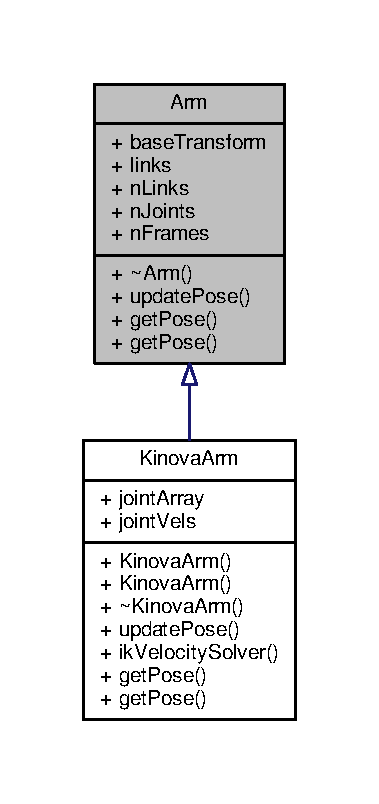
\includegraphics[width=182pt]{class_arm__inherit__graph}
\end{center}
\end{figure}


Collaboration diagram for Arm\+:\nopagebreak
\begin{figure}[H]
\begin{center}
\leavevmode
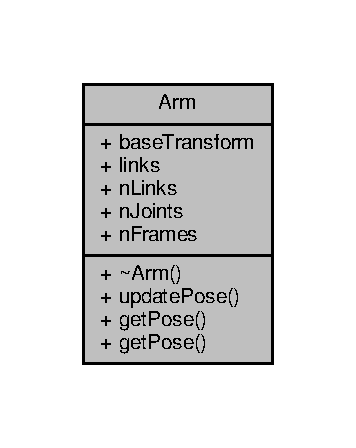
\includegraphics[width=171pt]{class_arm__coll__graph}
\end{center}
\end{figure}
\subsection*{Public Member Functions}
\begin{DoxyCompactItemize}
\item 
virtual \hyperlink{class_arm_ae1bcf12831b42e93d431efe3b7910b5e}{$\sim$\+Arm} ()
\item 
virtual bool \hyperlink{class_arm_a9bfe3a3f230c8fa8a39f88cce2d6b597}{update\+Pose} (std\+::vector$<$ double $>$ joint\+Positions)
\item 
virtual Eigen\+::\+Matrix4d \hyperlink{class_arm_af89cd963a4321584dfb8f9715c02f5be}{get\+Pose} (void)=0
\begin{DoxyCompactList}\small\item\em Used to get the endeffector frame of the manipulator. \end{DoxyCompactList}\item 
virtual Eigen\+::\+Matrix4d \hyperlink{class_arm_a994d35ca0dae04725fe0921c4f7d7e38}{get\+Pose} (int frame\+Number)=0
\begin{DoxyCompactList}\small\item\em Used to get the frame. \end{DoxyCompactList}\end{DoxyCompactItemize}
\subsection*{Public Attributes}
\begin{DoxyCompactItemize}
\item 
Eigen\+::\+Matrix4d \hyperlink{class_arm_ab568839905191e1e5abb83119a4a445d}{base\+Transform}
\begin{DoxyCompactList}\small\item\em The homogeneous transformation from the world to arm base frame. \end{DoxyCompactList}\item 
std\+::vector$<$ \hyperlink{class_primitive}{Primitive} $\ast$ $>$ \hyperlink{class_arm_a427fb95641bb8d0886b2849f0bda36be}{links}
\begin{DoxyCompactList}\small\item\em The list of link primitives that represent the manipulator. \end{DoxyCompactList}\item 
int \hyperlink{class_arm_a911ba9a8c719c090a305f88ab0ae7490}{n\+Links}
\begin{DoxyCompactList}\small\item\em The number of links in the chain. \end{DoxyCompactList}\item 
int \hyperlink{class_arm_ac3734a2ca38b0312fd42894ab6886bc9}{n\+Joints}
\begin{DoxyCompactList}\small\item\em The number of joints in the chain. \end{DoxyCompactList}\item 
int \hyperlink{class_arm_ac7955a5e8e9c6681b55d0d80d7e31df7}{n\+Frames}
\begin{DoxyCompactList}\small\item\em The number of frames in the arm. \end{DoxyCompactList}\end{DoxyCompactItemize}


\subsection{Detailed Description}
A pure virtual class that represents a robotic manipulator

This class is an interface class and so the developer is to implement this class to suit the type of robotic manipulator used 

Definition at line 16 of file arm.\+h.



\subsection{Constructor \& Destructor Documentation}
\index{Arm@{Arm}!````~Arm@{$\sim$\+Arm}}
\index{````~Arm@{$\sim$\+Arm}!Arm@{Arm}}
\subsubsection[{\texorpdfstring{$\sim$\+Arm()}{~Arm()}}]{\setlength{\rightskip}{0pt plus 5cm}Arm\+::$\sim$\+Arm (
\begin{DoxyParamCaption}
{}
\end{DoxyParamCaption}
)\hspace{0.3cm}{\ttfamily [virtual]}}\hypertarget{class_arm_ae1bcf12831b42e93d431efe3b7910b5e}{}\label{class_arm_ae1bcf12831b42e93d431efe3b7910b5e}


Definition at line 5 of file arm.\+cpp.



\subsection{Member Function Documentation}
\index{Arm@{Arm}!get\+Pose@{get\+Pose}}
\index{get\+Pose@{get\+Pose}!Arm@{Arm}}
\subsubsection[{\texorpdfstring{get\+Pose(void)=0}{getPose(void)=0}}]{\setlength{\rightskip}{0pt plus 5cm}virtual Eigen\+::\+Matrix4d Arm\+::get\+Pose (
\begin{DoxyParamCaption}
\item[{void}]{}
\end{DoxyParamCaption}
)\hspace{0.3cm}{\ttfamily [pure virtual]}}\hypertarget{class_arm_af89cd963a4321584dfb8f9715c02f5be}{}\label{class_arm_af89cd963a4321584dfb8f9715c02f5be}


Used to get the endeffector frame of the manipulator. 



Implemented in \hyperlink{class_kinova_arm_aea7c01f72eb70387ff71ca130db3bd3f}{Kinova\+Arm}.

\index{Arm@{Arm}!get\+Pose@{get\+Pose}}
\index{get\+Pose@{get\+Pose}!Arm@{Arm}}
\subsubsection[{\texorpdfstring{get\+Pose(int frame\+Number)=0}{getPose(int frameNumber)=0}}]{\setlength{\rightskip}{0pt plus 5cm}virtual Eigen\+::\+Matrix4d Arm\+::get\+Pose (
\begin{DoxyParamCaption}
\item[{int}]{frame\+Number}
\end{DoxyParamCaption}
)\hspace{0.3cm}{\ttfamily [pure virtual]}}\hypertarget{class_arm_a994d35ca0dae04725fe0921c4f7d7e38}{}\label{class_arm_a994d35ca0dae04725fe0921c4f7d7e38}


Used to get the frame. 



Implemented in \hyperlink{class_kinova_arm_ae6b5c17c1b7b79bc3de00e8d38b80999}{Kinova\+Arm}.

\index{Arm@{Arm}!update\+Pose@{update\+Pose}}
\index{update\+Pose@{update\+Pose}!Arm@{Arm}}
\subsubsection[{\texorpdfstring{update\+Pose(std\+::vector$<$ double $>$ joint\+Positions)}{updatePose(std::vector< double > jointPositions)}}]{\setlength{\rightskip}{0pt plus 5cm}bool Arm\+::update\+Pose (
\begin{DoxyParamCaption}
\item[{std\+::vector$<$ double $>$}]{joint\+Positions}
\end{DoxyParamCaption}
)\hspace{0.3cm}{\ttfamily [virtual]}}\hypertarget{class_arm_a9bfe3a3f230c8fa8a39f88cce2d6b597}{}\label{class_arm_a9bfe3a3f230c8fa8a39f88cce2d6b597}
A function to update the current virtual representation of the arm


\begin{DoxyParams}{Parameters}
{\em joint\+Positions} & The angular positions of the arm joints in order of the joint in radians \\
\hline
\end{DoxyParams}
\begin{DoxyReturn}{Returns}
The boolean true for a successful update, False otherwise 
\end{DoxyReturn}


Reimplemented in \hyperlink{class_kinova_arm_a3374988c7b3d9ae8773bc63f950629f7}{Kinova\+Arm}.



Definition at line 6 of file arm.\+cpp.



\subsection{Member Data Documentation}
\index{Arm@{Arm}!base\+Transform@{base\+Transform}}
\index{base\+Transform@{base\+Transform}!Arm@{Arm}}
\subsubsection[{\texorpdfstring{base\+Transform}{baseTransform}}]{\setlength{\rightskip}{0pt plus 5cm}Eigen\+::\+Matrix4d Arm\+::base\+Transform}\hypertarget{class_arm_ab568839905191e1e5abb83119a4a445d}{}\label{class_arm_ab568839905191e1e5abb83119a4a445d}


The homogeneous transformation from the world to arm base frame. 



Definition at line 38 of file arm.\+h.

\index{Arm@{Arm}!links@{links}}
\index{links@{links}!Arm@{Arm}}
\subsubsection[{\texorpdfstring{links}{links}}]{\setlength{\rightskip}{0pt plus 5cm}std\+::vector$<${\bf Primitive}$\ast$$>$ Arm\+::links}\hypertarget{class_arm_a427fb95641bb8d0886b2849f0bda36be}{}\label{class_arm_a427fb95641bb8d0886b2849f0bda36be}


The list of link primitives that represent the manipulator. 



Definition at line 41 of file arm.\+h.

\index{Arm@{Arm}!n\+Frames@{n\+Frames}}
\index{n\+Frames@{n\+Frames}!Arm@{Arm}}
\subsubsection[{\texorpdfstring{n\+Frames}{nFrames}}]{\setlength{\rightskip}{0pt plus 5cm}int Arm\+::n\+Frames}\hypertarget{class_arm_ac7955a5e8e9c6681b55d0d80d7e31df7}{}\label{class_arm_ac7955a5e8e9c6681b55d0d80d7e31df7}


The number of frames in the arm. 



Definition at line 47 of file arm.\+h.

\index{Arm@{Arm}!n\+Joints@{n\+Joints}}
\index{n\+Joints@{n\+Joints}!Arm@{Arm}}
\subsubsection[{\texorpdfstring{n\+Joints}{nJoints}}]{\setlength{\rightskip}{0pt plus 5cm}int Arm\+::n\+Joints}\hypertarget{class_arm_ac3734a2ca38b0312fd42894ab6886bc9}{}\label{class_arm_ac3734a2ca38b0312fd42894ab6886bc9}


The number of joints in the chain. 



Definition at line 45 of file arm.\+h.

\index{Arm@{Arm}!n\+Links@{n\+Links}}
\index{n\+Links@{n\+Links}!Arm@{Arm}}
\subsubsection[{\texorpdfstring{n\+Links}{nLinks}}]{\setlength{\rightskip}{0pt plus 5cm}int Arm\+::n\+Links}\hypertarget{class_arm_a911ba9a8c719c090a305f88ab0ae7490}{}\label{class_arm_a911ba9a8c719c090a305f88ab0ae7490}


The number of links in the chain. 



Definition at line 43 of file arm.\+h.



The documentation for this class was generated from the following files\+:\begin{DoxyCompactItemize}
\item 
\hyperlink{arm_8h}{arm.\+h}\item 
\hyperlink{arm_8cpp}{arm.\+cpp}\end{DoxyCompactItemize}

\hypertarget{class_arm_controller}{}\section{Arm\+Controller Class Reference}
\label{class_arm_controller}\index{Arm\+Controller@{Arm\+Controller}}


{\ttfamily \#include $<$arm\+\_\+controller.\+h$>$}



Collaboration diagram for Arm\+Controller\+:\nopagebreak
\begin{figure}[H]
\begin{center}
\leavevmode
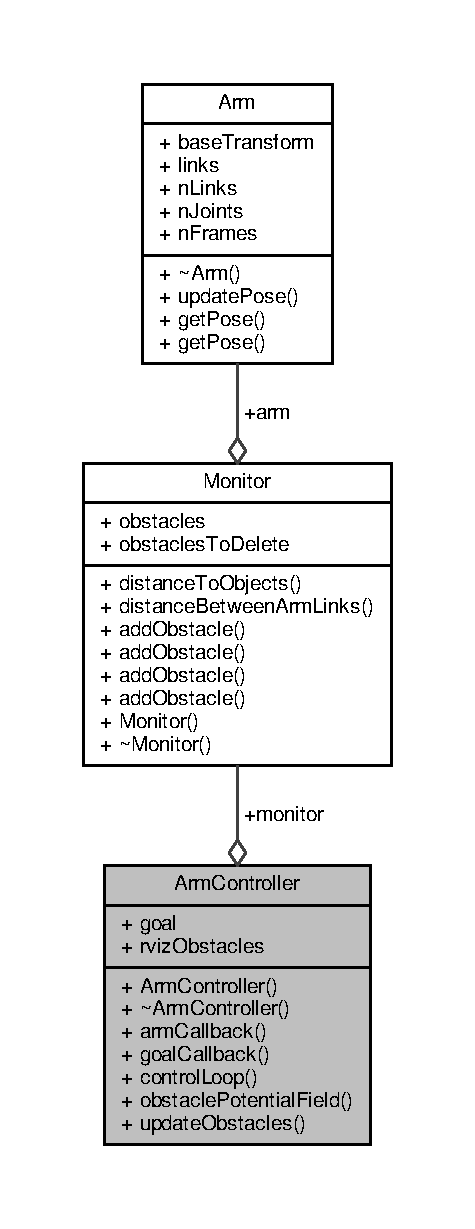
\includegraphics[width=157pt]{class_arm_controller__coll__graph}
\end{center}
\end{figure}
\subsection*{Public Member Functions}
\begin{DoxyCompactItemize}
\item 
\hyperlink{class_arm_controller_a27a8d755210b8e3bd96217ea8080b327}{Arm\+Controller} (\hyperlink{class_monitor}{Monitor} $\ast$monitor\+Object, double k, double d, double gamma, double beta)
\item 
\hyperlink{class_arm_controller_ad2b44ab21366148d89980e942b26d232}{$\sim$\+Arm\+Controller} ()\hypertarget{class_arm_controller_ad2b44ab21366148d89980e942b26d232}{}\label{class_arm_controller_ad2b44ab21366148d89980e942b26d232}

\begin{DoxyCompactList}\small\item\em \hyperlink{class_kinova_arm}{Kinova\+Arm} Destructor. \end{DoxyCompactList}\item 
void \hyperlink{class_arm_controller_a29defeb3894d62016523a99b63320a22}{arm\+Callback} (const sensor\+\_\+msgs\+::\+Joint\+State\+::\+Const\+Ptr \&msg)
\item 
void \hyperlink{class_arm_controller_acbd85ddee96c8d6fd76728c68fb12d3c}{goal\+Callback} (const geometry\+\_\+msgs\+::\+Point\+::\+Const\+Ptr \&msg)
\item 
K\+D\+L\+::\+Twist \hyperlink{class_arm_controller_ad7e00a70c968a23087415b1bd0ac8bf1}{control\+Loop} (void)
\item 
Eigen\+::\+Vector3d \hyperlink{class_arm_controller_ad0b1f28333e2a3be76258153a745803d}{obstacle\+Potential\+Field} (Eigen\+::\+Vector3d current\+Position, Eigen\+::\+Vector3d velocity)
\item 
void \hyperlink{class_arm_controller_a17d05bd19286dc4e04355e3d4f6bb372}{update\+Obstacles} (const visualization\+\_\+msgs\+::\+Marker\+::\+Const\+Ptr \&msg)
\end{DoxyCompactItemize}
\subsection*{Public Attributes}
\begin{DoxyCompactItemize}
\item 
\hyperlink{class_monitor}{Monitor} $\ast$ \hyperlink{class_arm_controller_a939747279bba6db315f80092a74c2629}{monitor}\hypertarget{class_arm_controller_a939747279bba6db315f80092a74c2629}{}\label{class_arm_controller_a939747279bba6db315f80092a74c2629}

\begin{DoxyCompactList}\small\item\em The monitor class used to perform collision monitoring. \end{DoxyCompactList}\item 
Eigen\+::\+Vector3d \hyperlink{class_arm_controller_a5246aa4a2072b1511d510717fc253f88}{goal}\hypertarget{class_arm_controller_a5246aa4a2072b1511d510717fc253f88}{}\label{class_arm_controller_a5246aa4a2072b1511d510717fc253f88}

\begin{DoxyCompactList}\small\item\em The goal point of the endeffector. \end{DoxyCompactList}\item 
std\+::vector$<$ \hyperlink{class_rviz_obstacle}{Rviz\+Obstacle} $\ast$ $>$ \hyperlink{class_arm_controller_ab94a1abce40096f6476404d49d00860f}{rviz\+Obstacles}\hypertarget{class_arm_controller_ab94a1abce40096f6476404d49d00860f}{}\label{class_arm_controller_ab94a1abce40096f6476404d49d00860f}

\begin{DoxyCompactList}\small\item\em A list of obstacles that are displayed in rviz. \end{DoxyCompactList}\end{DoxyCompactItemize}


\subsection{Detailed Description}
\hyperlink{class_arm}{Arm} controller class to demonstate the use of the Collision monitoring library.

The class uses the monitor class from the custom library to control a 7\+D\+OF kinova arm implementing the paper\+: \mbox{[}1\mbox{]}H. Hoffmann, P. Pastor, D.-\/H. Park, and S. Schaal, “\+Biologically-\/inspired dynamical systems for movement generation\+: Automatic real-\/time goal adaptation and obstacle avoidance,” in 2009 I\+E\+EE International Conference on Robotics and Automation, Kobe, May 2009, pp. 2587–2592, doi\+: 10.\+1109/\+R\+O\+B\+OT.2009.\+5152423. 

Definition at line 83 of file arm\+\_\+controller.\+h.



\subsection{Constructor \& Destructor Documentation}
\index{Arm\+Controller@{Arm\+Controller}!Arm\+Controller@{Arm\+Controller}}
\index{Arm\+Controller@{Arm\+Controller}!Arm\+Controller@{Arm\+Controller}}
\subsubsection[{\texorpdfstring{Arm\+Controller(\+Monitor $\ast$monitor\+Object, double k, double d, double gamma, double beta)}{ArmController(Monitor *monitorObject, double k, double d, double gamma, double beta)}}]{\setlength{\rightskip}{0pt plus 5cm}Arm\+Controller\+::\+Arm\+Controller (
\begin{DoxyParamCaption}
\item[{{\bf Monitor} $\ast$}]{monitor\+Object, }
\item[{double}]{k, }
\item[{double}]{d, }
\item[{double}]{gamma, }
\item[{double}]{beta}
\end{DoxyParamCaption}
)}\hypertarget{class_arm_controller_a27a8d755210b8e3bd96217ea8080b327}{}\label{class_arm_controller_a27a8d755210b8e3bd96217ea8080b327}
\hyperlink{class_kinova_arm}{Kinova\+Arm} constructor


\begin{DoxyParams}{Parameters}
{\em monitor\+Object} & The monitor instance used to get the distance from the arm to any obstacles \\
\hline
{\em k} & Costant for the obstacle avoidance algorithim \\
\hline
{\em d} & Costant for the obstacle avoidance algorithim \\
\hline
{\em gamma} & Costant for the obstacle avoidance algorithim \\
\hline
{\em beta} & Costant for the obstacle avoidance algorithim \\
\hline
\end{DoxyParams}
\begin{DoxyReturn}{Returns}
An instance of Collision\+Monitor class 
\end{DoxyReturn}


Definition at line 6 of file arm\+\_\+controller.\+cpp.



\subsection{Member Function Documentation}
\index{Arm\+Controller@{Arm\+Controller}!arm\+Callback@{arm\+Callback}}
\index{arm\+Callback@{arm\+Callback}!Arm\+Controller@{Arm\+Controller}}
\subsubsection[{\texorpdfstring{arm\+Callback(const sensor\+\_\+msgs\+::\+Joint\+State\+::\+Const\+Ptr \&msg)}{armCallback(const sensor_msgs::JointState::ConstPtr &msg)}}]{\setlength{\rightskip}{0pt plus 5cm}void Arm\+Controller\+::arm\+Callback (
\begin{DoxyParamCaption}
\item[{const sensor\+\_\+msgs\+::\+Joint\+State\+::\+Const\+Ptr \&}]{msg}
\end{DoxyParamCaption}
)}\hypertarget{class_arm_controller_a29defeb3894d62016523a99b63320a22}{}\label{class_arm_controller_a29defeb3894d62016523a99b63320a22}
Callback function updating the arm positions


\begin{DoxyParams}{Parameters}
{\em msg} & The ros sensor messsage containing the joint angles \\
\hline
\end{DoxyParams}


Definition at line 53 of file arm\+\_\+controller.\+cpp.

\index{Arm\+Controller@{Arm\+Controller}!control\+Loop@{control\+Loop}}
\index{control\+Loop@{control\+Loop}!Arm\+Controller@{Arm\+Controller}}
\subsubsection[{\texorpdfstring{control\+Loop(void)}{controlLoop(void)}}]{\setlength{\rightskip}{0pt plus 5cm}K\+D\+L\+::\+Twist Arm\+Controller\+::control\+Loop (
\begin{DoxyParamCaption}
\item[{void}]{}
\end{DoxyParamCaption}
)}\hypertarget{class_arm_controller_ad7e00a70c968a23087415b1bd0ac8bf1}{}\label{class_arm_controller_ad7e00a70c968a23087415b1bd0ac8bf1}
Function that uses internal parameters to send instructions to arm

This is where the obstacle avoidance is implemented and is based off of the paper\+: 

Definition at line 179 of file arm\+\_\+controller.\+cpp.

\index{Arm\+Controller@{Arm\+Controller}!goal\+Callback@{goal\+Callback}}
\index{goal\+Callback@{goal\+Callback}!Arm\+Controller@{Arm\+Controller}}
\subsubsection[{\texorpdfstring{goal\+Callback(const geometry\+\_\+msgs\+::\+Point\+::\+Const\+Ptr \&msg)}{goalCallback(const geometry_msgs::Point::ConstPtr &msg)}}]{\setlength{\rightskip}{0pt plus 5cm}void Arm\+Controller\+::goal\+Callback (
\begin{DoxyParamCaption}
\item[{const geometry\+\_\+msgs\+::\+Point\+::\+Const\+Ptr \&}]{msg}
\end{DoxyParamCaption}
)}\hypertarget{class_arm_controller_acbd85ddee96c8d6fd76728c68fb12d3c}{}\label{class_arm_controller_acbd85ddee96c8d6fd76728c68fb12d3c}
Callback function updating goal position of the arms endeffector


\begin{DoxyParams}{Parameters}
{\em msg} & The ros sensor messsage containing the goal position \\
\hline
\end{DoxyParams}


Definition at line 60 of file arm\+\_\+controller.\+cpp.

\index{Arm\+Controller@{Arm\+Controller}!obstacle\+Potential\+Field@{obstacle\+Potential\+Field}}
\index{obstacle\+Potential\+Field@{obstacle\+Potential\+Field}!Arm\+Controller@{Arm\+Controller}}
\subsubsection[{\texorpdfstring{obstacle\+Potential\+Field(\+Eigen\+::\+Vector3d current\+Position, Eigen\+::\+Vector3d velocity)}{obstaclePotentialField(Eigen::Vector3d currentPosition, Eigen::Vector3d velocity)}}]{\setlength{\rightskip}{0pt plus 5cm}Eigen\+::\+Vector3d Arm\+Controller\+::obstacle\+Potential\+Field (
\begin{DoxyParamCaption}
\item[{Eigen\+::\+Vector3d}]{current\+Position, }
\item[{Eigen\+::\+Vector3d}]{velocity}
\end{DoxyParamCaption}
)}\hypertarget{class_arm_controller_ad0b1f28333e2a3be76258153a745803d}{}\label{class_arm_controller_ad0b1f28333e2a3be76258153a745803d}
Creates the obstacle potential feild value used in the control loop \mbox{[}1\mbox{]}


\begin{DoxyParams}{Parameters}
{\em current\+Position} & The current position of the endeffector \\
\hline
{\em velocity} & The current velocity of the endeffector \\
\hline
\end{DoxyParams}
\begin{DoxyReturn}{Returns}
The potential feild vector produced from the obstacles 
\end{DoxyReturn}


Definition at line 78 of file arm\+\_\+controller.\+cpp.

\index{Arm\+Controller@{Arm\+Controller}!update\+Obstacles@{update\+Obstacles}}
\index{update\+Obstacles@{update\+Obstacles}!Arm\+Controller@{Arm\+Controller}}
\subsubsection[{\texorpdfstring{update\+Obstacles(const visualization\+\_\+msgs\+::\+Marker\+::\+Const\+Ptr \&msg)}{updateObstacles(const visualization_msgs::Marker::ConstPtr &msg)}}]{\setlength{\rightskip}{0pt plus 5cm}void Arm\+Controller\+::update\+Obstacles (
\begin{DoxyParamCaption}
\item[{const visualization\+\_\+msgs\+::\+Marker\+::\+Const\+Ptr \&}]{msg}
\end{DoxyParamCaption}
)}\hypertarget{class_arm_controller_a17d05bd19286dc4e04355e3d4f6bb372}{}\label{class_arm_controller_a17d05bd19286dc4e04355e3d4f6bb372}
A callback function that updates or adds obstacles


\begin{DoxyParams}{Parameters}
{\em msg} & the ros marker message with the object parameters \\
\hline
\end{DoxyParams}


Definition at line 252 of file arm\+\_\+controller.\+cpp.



The documentation for this class was generated from the following files\+:\begin{DoxyCompactItemize}
\item 
arm\+\_\+controller.\+h\item 
arm\+\_\+controller.\+cpp\end{DoxyCompactItemize}

\hypertarget{class_capsule}{}\section{Capsule Class Reference}
\label{class_capsule}\index{Capsule@{Capsule}}


{\ttfamily \#include $<$primitives.\+h$>$}



Inheritance diagram for Capsule\+:\nopagebreak
\begin{figure}[H]
\begin{center}
\leavevmode
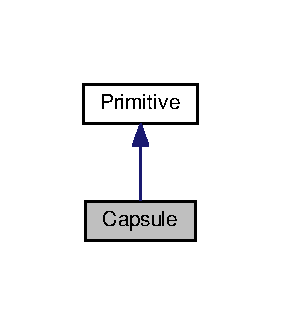
\includegraphics[width=135pt]{class_capsule__inherit__graph}
\end{center}
\end{figure}


Collaboration diagram for Capsule\+:\nopagebreak
\begin{figure}[H]
\begin{center}
\leavevmode
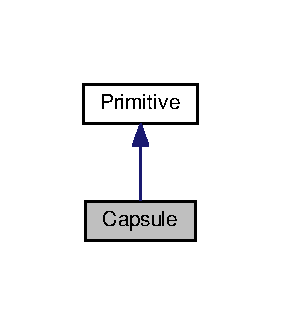
\includegraphics[width=135pt]{class_capsule__coll__graph}
\end{center}
\end{figure}
\subsection*{Public Member Functions}
\begin{DoxyCompactItemize}
\item 
\hyperlink{class_capsule_aab6d0827aa8179c3f258129161a67e2e}{Capsule} (Eigen\+::\+Matrix4d \hyperlink{class_primitive_ad8b2afbad412f6046783d155c88fe312}{pose}, double \hyperlink{class_capsule_af62f20ecfc37b4c8ae88dd505ca1f196}{length}, double \hyperlink{class_capsule_a9b7e591748a2b735b35d99a2d7792f39}{radius})
\item 
\hyperlink{class_capsule_a94838c4642111c07dbf83fdc775d1a68}{Capsule} (\hyperlink{class_capsule}{Capsule} $\ast$capsule)
\item 
float \hyperlink{class_capsule_a8ff7a408a608ee32dea8c187fce5dbea}{get\+Length} ()
\item 
float \hyperlink{class_capsule_a4e98e8545ea57fe682c5a2002bd49bdb}{get\+Radius} ()
\item 
void \hyperlink{class_capsule_ad569eae23b91f33e145f06745739e428}{get\+Shortest\+Direction} (Eigen\+::\+Vector3d \&shortest\+Direction, \hyperlink{class_primitive}{Primitive} $\ast$primitive)
\item 
void \hyperlink{class_capsule_a28274c18ef5a3b9ef869caa64d5f7d5e}{get\+Shortest\+Direction} (Eigen\+::\+Vector3d \&shortest\+Direction, \hyperlink{class_capsule}{Capsule} $\ast$capsule)
\item 
void \hyperlink{class_capsule_aae076a389170bd6644f479bfe9c243bc}{get\+Shortest\+Direction} (Eigen\+::\+Vector3d \&shortest\+Direction, \hyperlink{class_sphere}{Sphere} $\ast$sphere)
\item 
double \hyperlink{class_capsule_a43bcc7bb95425a4559f7fd0289ef8b45}{get\+Shortest\+Distance} (\hyperlink{class_primitive}{Primitive} $\ast$primitive)
\item 
double \hyperlink{class_capsule_ade8880442a9230f893c296f0681ae9ad}{get\+Shortest\+Distance} (\hyperlink{class_capsule}{Capsule} $\ast$capsule)
\item 
double \hyperlink{class_capsule_a71d7821f3e7f9ac972bceb06d82f529d}{get\+Shortest\+Distance} (\hyperlink{class_sphere}{Sphere} $\ast$sphere)
\end{DoxyCompactItemize}
\subsection*{Protected Attributes}
\begin{DoxyCompactItemize}
\item 
float \hyperlink{class_capsule_af62f20ecfc37b4c8ae88dd505ca1f196}{length}\hypertarget{class_capsule_af62f20ecfc37b4c8ae88dd505ca1f196}{}\label{class_capsule_af62f20ecfc37b4c8ae88dd505ca1f196}

\begin{DoxyCompactList}\small\item\em length of the capsule \end{DoxyCompactList}\item 
float \hyperlink{class_capsule_a9b7e591748a2b735b35d99a2d7792f39}{radius}\hypertarget{class_capsule_a9b7e591748a2b735b35d99a2d7792f39}{}\label{class_capsule_a9b7e591748a2b735b35d99a2d7792f39}

\begin{DoxyCompactList}\small\item\em radius of the capsule \end{DoxyCompactList}\end{DoxyCompactItemize}
\subsection*{Additional Inherited Members}


\subsection{Detailed Description}
The \hyperlink{class_capsule}{Capsule} class. A cylinder with two half spheres at both ends.

This class is a shape that inherits from primitive. It\textquotesingle{}s similar to a cylinder containing half spheres in the ends, making a capsule. 

Definition at line 205 of file primitives.\+h.



\subsection{Constructor \& Destructor Documentation}
\index{Capsule@{Capsule}!Capsule@{Capsule}}
\index{Capsule@{Capsule}!Capsule@{Capsule}}
\subsubsection[{\texorpdfstring{Capsule(\+Eigen\+::\+Matrix4d pose, double length, double radius)}{Capsule(Eigen::Matrix4d pose, double length, double radius)}}]{\setlength{\rightskip}{0pt plus 5cm}Capsule\+::\+Capsule (
\begin{DoxyParamCaption}
\item[{Eigen\+::\+Matrix4d}]{pose, }
\item[{double}]{length, }
\item[{double}]{radius}
\end{DoxyParamCaption}
)}\hypertarget{class_capsule_aab6d0827aa8179c3f258129161a67e2e}{}\label{class_capsule_aab6d0827aa8179c3f258129161a67e2e}
Constructor of \hyperlink{class_capsule}{Capsule} class


\begin{DoxyParams}{Parameters}
{\em pose} & start point of the line represented with a Matrix4d. \\
\hline
{\em length} & length of the capsule \\
\hline
{\em radius} & radius of the capsule \\
\hline
\end{DoxyParams}


Definition at line 119 of file primitives.\+cpp.

\index{Capsule@{Capsule}!Capsule@{Capsule}}
\index{Capsule@{Capsule}!Capsule@{Capsule}}
\subsubsection[{\texorpdfstring{Capsule(\+Capsule $\ast$capsule)}{Capsule(Capsule *capsule)}}]{\setlength{\rightskip}{0pt plus 5cm}Capsule\+::\+Capsule (
\begin{DoxyParamCaption}
\item[{{\bf Capsule} $\ast$}]{capsule}
\end{DoxyParamCaption}
)}\hypertarget{class_capsule_a94838c4642111c07dbf83fdc775d1a68}{}\label{class_capsule_a94838c4642111c07dbf83fdc775d1a68}
Copy onstructor of \hyperlink{class_capsule}{Capsule} class


\begin{DoxyParams}{Parameters}
{\em capsule} & the capsule instance to copy \\
\hline
\end{DoxyParams}


Definition at line 125 of file primitives.\+cpp.



\subsection{Member Function Documentation}
\index{Capsule@{Capsule}!get\+Length@{get\+Length}}
\index{get\+Length@{get\+Length}!Capsule@{Capsule}}
\subsubsection[{\texorpdfstring{get\+Length()}{getLength()}}]{\setlength{\rightskip}{0pt plus 5cm}float Capsule\+::get\+Length (
\begin{DoxyParamCaption}
{}
\end{DoxyParamCaption}
)}\hypertarget{class_capsule_a8ff7a408a608ee32dea8c187fce5dbea}{}\label{class_capsule_a8ff7a408a608ee32dea8c187fce5dbea}
Getter of length

\begin{DoxyReturn}{Returns}
the length of the capsule 
\end{DoxyReturn}


Definition at line 135 of file primitives.\+cpp.

\index{Capsule@{Capsule}!get\+Radius@{get\+Radius}}
\index{get\+Radius@{get\+Radius}!Capsule@{Capsule}}
\subsubsection[{\texorpdfstring{get\+Radius()}{getRadius()}}]{\setlength{\rightskip}{0pt plus 5cm}float Capsule\+::get\+Radius (
\begin{DoxyParamCaption}
{}
\end{DoxyParamCaption}
)}\hypertarget{class_capsule_a4e98e8545ea57fe682c5a2002bd49bdb}{}\label{class_capsule_a4e98e8545ea57fe682c5a2002bd49bdb}
Getter of radius

\begin{DoxyReturn}{Returns}
the radius of the capsule 
\end{DoxyReturn}


Definition at line 139 of file primitives.\+cpp.

\index{Capsule@{Capsule}!get\+Shortest\+Direction@{get\+Shortest\+Direction}}
\index{get\+Shortest\+Direction@{get\+Shortest\+Direction}!Capsule@{Capsule}}
\subsubsection[{\texorpdfstring{get\+Shortest\+Direction(\+Eigen\+::\+Vector3d \&shortest\+Direction, Primitive $\ast$primitive)}{getShortestDirection(Eigen::Vector3d &shortestDirection, Primitive *primitive)}}]{\setlength{\rightskip}{0pt plus 5cm}void Capsule\+::get\+Shortest\+Direction (
\begin{DoxyParamCaption}
\item[{Eigen\+::\+Vector3d \&}]{shortest\+Direction, }
\item[{{\bf Primitive} $\ast$}]{primitive}
\end{DoxyParamCaption}
)\hspace{0.3cm}{\ttfamily [virtual]}}\hypertarget{class_capsule_ad569eae23b91f33e145f06745739e428}{}\label{class_capsule_ad569eae23b91f33e145f06745739e428}
Performs a dynamic cast to overload the direction functions

This method takes an object that inherits from primitive and performs a dynamic cast to call the correct get\+Shortest\+Direction method depending on the class of the shape.


\begin{DoxyParams}[1]{Parameters}
 & {\em primitive} & address of the primitive object. \\
\hline
\mbox{\tt out}  & {\em shortest\+Direction} & a vector in 3D that represents the closes direction between this and the second primitive. \\
\hline
\end{DoxyParams}


Implements \hyperlink{class_primitive_ae37bbdf5271bf278b19888e0428579a8}{Primitive}.



Definition at line 143 of file primitives.\+cpp.

\index{Capsule@{Capsule}!get\+Shortest\+Direction@{get\+Shortest\+Direction}}
\index{get\+Shortest\+Direction@{get\+Shortest\+Direction}!Capsule@{Capsule}}
\subsubsection[{\texorpdfstring{get\+Shortest\+Direction(\+Eigen\+::\+Vector3d \&shortest\+Direction, Capsule $\ast$capsule)}{getShortestDirection(Eigen::Vector3d &shortestDirection, Capsule *capsule)}}]{\setlength{\rightskip}{0pt plus 5cm}void Capsule\+::get\+Shortest\+Direction (
\begin{DoxyParamCaption}
\item[{Eigen\+::\+Vector3d \&}]{shortest\+Direction, }
\item[{{\bf Capsule} $\ast$}]{capsule}
\end{DoxyParamCaption}
)\hspace{0.3cm}{\ttfamily [virtual]}}\hypertarget{class_capsule_a28274c18ef5a3b9ef869caa64d5f7d5e}{}\label{class_capsule_a28274c18ef5a3b9ef869caa64d5f7d5e}
Finds the shortest distance between this primitive and a \hyperlink{class_capsule}{Capsule} primitive

This method takes a capsule object and returns the closest direction between this primitive and a capsule object.


\begin{DoxyParams}[1]{Parameters}
 & {\em capsule} & address of the primitive object \\
\hline
\mbox{\tt out}  & {\em shortest\+Direction} & a vector in 3D that represents the closes direction between the primitive and capsule \\
\hline
\end{DoxyParams}


Implements \hyperlink{class_primitive_af9bd724a6618bd76e41e5682caa25023}{Primitive}.



Definition at line 157 of file primitives.\+cpp.

\index{Capsule@{Capsule}!get\+Shortest\+Direction@{get\+Shortest\+Direction}}
\index{get\+Shortest\+Direction@{get\+Shortest\+Direction}!Capsule@{Capsule}}
\subsubsection[{\texorpdfstring{get\+Shortest\+Direction(\+Eigen\+::\+Vector3d \&shortest\+Direction, Sphere $\ast$sphere)}{getShortestDirection(Eigen::Vector3d &shortestDirection, Sphere *sphere)}}]{\setlength{\rightskip}{0pt plus 5cm}void Capsule\+::get\+Shortest\+Direction (
\begin{DoxyParamCaption}
\item[{Eigen\+::\+Vector3d \&}]{shortest\+Direction, }
\item[{{\bf Sphere} $\ast$}]{sphere}
\end{DoxyParamCaption}
)\hspace{0.3cm}{\ttfamily [virtual]}}\hypertarget{class_capsule_aae076a389170bd6644f479bfe9c243bc}{}\label{class_capsule_aae076a389170bd6644f479bfe9c243bc}
Finds the shortest distance between this primitive and a \hyperlink{class_sphere}{Sphere} primitive

This method takes a capsule object and returns the closest direction between this primitive and a sphere object. returns a Vector3d.


\begin{DoxyParams}[1]{Parameters}
 & {\em sphere} & address of the primitive object \\
\hline
\mbox{\tt out}  & {\em shortest\+Direction} & a vector in 3D that represents the closes direction between the primitive and sphere \\
\hline
\end{DoxyParams}


Implements \hyperlink{class_primitive_a3f1bc91de29fa904657c1ba4c40eee53}{Primitive}.



Definition at line 232 of file primitives.\+cpp.

\index{Capsule@{Capsule}!get\+Shortest\+Distance@{get\+Shortest\+Distance}}
\index{get\+Shortest\+Distance@{get\+Shortest\+Distance}!Capsule@{Capsule}}
\subsubsection[{\texorpdfstring{get\+Shortest\+Distance(\+Primitive $\ast$primitive)}{getShortestDistance(Primitive *primitive)}}]{\setlength{\rightskip}{0pt plus 5cm}double Capsule\+::get\+Shortest\+Distance (
\begin{DoxyParamCaption}
\item[{{\bf Primitive} $\ast$}]{primitive}
\end{DoxyParamCaption}
)\hspace{0.3cm}{\ttfamily [virtual]}}\hypertarget{class_capsule_a43bcc7bb95425a4559f7fd0289ef8b45}{}\label{class_capsule_a43bcc7bb95425a4559f7fd0289ef8b45}
Performs a dynamic cast to overload the distance functions

This method takes an object that inherits from primitive and performs a dynamic cast to call the correct get\+Shortest\+Distance method depending on the class of the shape. returns a double value.


\begin{DoxyParams}{Parameters}
{\em primitive} & address of the primitive object. \\
\hline
\end{DoxyParams}
\begin{DoxyReturn}{Returns}
the closest distance between this and the second primitive. 
\end{DoxyReturn}


Implements \hyperlink{class_primitive_a340b3e5540b910480ada939383985d66}{Primitive}.



Definition at line 248 of file primitives.\+cpp.

\index{Capsule@{Capsule}!get\+Shortest\+Distance@{get\+Shortest\+Distance}}
\index{get\+Shortest\+Distance@{get\+Shortest\+Distance}!Capsule@{Capsule}}
\subsubsection[{\texorpdfstring{get\+Shortest\+Distance(\+Capsule $\ast$capsule)}{getShortestDistance(Capsule *capsule)}}]{\setlength{\rightskip}{0pt plus 5cm}double Capsule\+::get\+Shortest\+Distance (
\begin{DoxyParamCaption}
\item[{{\bf Capsule} $\ast$}]{capsule}
\end{DoxyParamCaption}
)\hspace{0.3cm}{\ttfamily [virtual]}}\hypertarget{class_capsule_ade8880442a9230f893c296f0681ae9ad}{}\label{class_capsule_ade8880442a9230f893c296f0681ae9ad}
Finds the shortest distance between this primitive and a \hyperlink{class_capsule}{Capsule} primitive

This method takes a capsule object and returns the closest distance between this primitive and a capsule object. returns a double value.


\begin{DoxyParams}{Parameters}
{\em capsule} & address of the primitive object \\
\hline
\end{DoxyParams}
\begin{DoxyReturn}{Returns}
the closest distance between the primitive and capsule 
\end{DoxyReturn}


Implements \hyperlink{class_primitive_a46e60acfe4c005c0ec94e1e8b82d36db}{Primitive}.



Definition at line 262 of file primitives.\+cpp.

\index{Capsule@{Capsule}!get\+Shortest\+Distance@{get\+Shortest\+Distance}}
\index{get\+Shortest\+Distance@{get\+Shortest\+Distance}!Capsule@{Capsule}}
\subsubsection[{\texorpdfstring{get\+Shortest\+Distance(\+Sphere $\ast$sphere)}{getShortestDistance(Sphere *sphere)}}]{\setlength{\rightskip}{0pt plus 5cm}double Capsule\+::get\+Shortest\+Distance (
\begin{DoxyParamCaption}
\item[{{\bf Sphere} $\ast$}]{sphere}
\end{DoxyParamCaption}
)\hspace{0.3cm}{\ttfamily [virtual]}}\hypertarget{class_capsule_a71d7821f3e7f9ac972bceb06d82f529d}{}\label{class_capsule_a71d7821f3e7f9ac972bceb06d82f529d}
Finds the shortest distance between this primitive and a \hyperlink{class_sphere}{Sphere} primitive

This method takes a capsule object and returns the closest distance between this primitive and a sphere object. returns a double value.


\begin{DoxyParams}{Parameters}
{\em sphere} & address of the primitive object \\
\hline
\end{DoxyParams}
\begin{DoxyReturn}{Returns}
the closest distance between the primitive and sphere 
\end{DoxyReturn}


Implements \hyperlink{class_primitive_adaac4fc4fedf9cd76d4eb9c77e9ae560}{Primitive}.



Definition at line 272 of file primitives.\+cpp.



The documentation for this class was generated from the following files\+:\begin{DoxyCompactItemize}
\item 
primitives.\+h\item 
primitives.\+cpp\end{DoxyCompactItemize}

\hypertarget{class_kinova_arm}{}\section{Kinova\+Arm Class Reference}
\label{class_kinova_arm}\index{Kinova\+Arm@{Kinova\+Arm}}


{\ttfamily \#include $<$kinova\+\_\+arm.\+h$>$}



Inheritance diagram for Kinova\+Arm\+:\nopagebreak
\begin{figure}[H]
\begin{center}
\leavevmode
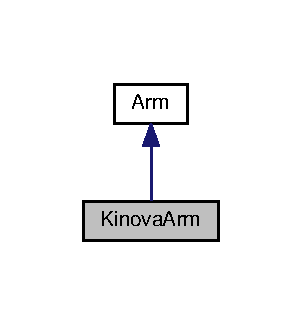
\includegraphics[width=145pt]{class_kinova_arm__inherit__graph}
\end{center}
\end{figure}


Collaboration diagram for Kinova\+Arm\+:\nopagebreak
\begin{figure}[H]
\begin{center}
\leavevmode
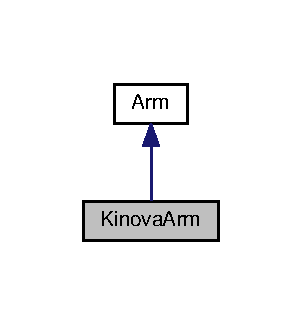
\includegraphics[width=145pt]{class_kinova_arm__coll__graph}
\end{center}
\end{figure}
\subsection*{Public Member Functions}
\begin{DoxyCompactItemize}
\item 
\hyperlink{class_kinova_arm_abbbe90c0d43bf6665d62bdf6c1ef398f}{Kinova\+Arm} (std\+::string urdf\+\_\+filename)
\item 
\hyperlink{class_kinova_arm_a5ca50dcf1c211aea4986bc5a04f37331}{Kinova\+Arm} (std\+::string urdf\+\_\+filename, Eigen\+::\+Matrix4d input\+Base\+Transform)
\item 
\hyperlink{class_kinova_arm_a9d5b485d8137a0b27e98a0c1c4d67861}{$\sim$\+Kinova\+Arm} ()\hypertarget{class_kinova_arm_a9d5b485d8137a0b27e98a0c1c4d67861}{}\label{class_kinova_arm_a9d5b485d8137a0b27e98a0c1c4d67861}

\begin{DoxyCompactList}\small\item\em \hyperlink{class_kinova_arm}{Kinova\+Arm} Destructor. \end{DoxyCompactList}\item 
bool \hyperlink{class_kinova_arm_a3374988c7b3d9ae8773bc63f950629f7}{update\+Pose} (std\+::vector$<$ double $>$ joint\+Positions)
\item 
std\+::vector$<$ double $>$ \hyperlink{class_kinova_arm_a0a5a3bd128b420d58d92d242c075db92}{ik\+Velocity\+Solver} (K\+D\+L\+::\+Twist twist)
\item 
Eigen\+::\+Matrix4d \hyperlink{class_kinova_arm_aea7c01f72eb70387ff71ca130db3bd3f}{get\+Pose} (void)
\item 
Eigen\+::\+Matrix4d \hyperlink{class_kinova_arm_ae6b5c17c1b7b79bc3de00e8d38b80999}{get\+Pose} (int frame\+Number)
\end{DoxyCompactItemize}
\subsection*{Public Attributes}
\begin{DoxyCompactItemize}
\item 
K\+D\+L\+::\+Jnt\+Array \hyperlink{class_kinova_arm_a47ddba255203039c2d7d3ceb48b2c4ac}{joint\+Array}\hypertarget{class_kinova_arm_a47ddba255203039c2d7d3ceb48b2c4ac}{}\label{class_kinova_arm_a47ddba255203039c2d7d3ceb48b2c4ac}

\begin{DoxyCompactList}\small\item\em The K\+DL joint array to hold the joint angles. \end{DoxyCompactList}\item 
K\+D\+L\+::\+Jnt\+Array \hyperlink{class_kinova_arm_adeab92c27d6555029a30f5bcbba8bfab}{joint\+Vels}\hypertarget{class_kinova_arm_adeab92c27d6555029a30f5bcbba8bfab}{}\label{class_kinova_arm_adeab92c27d6555029a30f5bcbba8bfab}

\begin{DoxyCompactList}\small\item\em The K\+DL joint array to hold the joint velocities. \end{DoxyCompactList}\end{DoxyCompactItemize}


\subsection{Detailed Description}
An implementation of the \hyperlink{class_arm}{Arm} interface.

This implementation is specifically for the K\+I\+N\+O\+VA arm in the H\+B\+RS robotics lab. 

Definition at line 30 of file kinova\+\_\+arm.\+h.



\subsection{Constructor \& Destructor Documentation}
\index{Kinova\+Arm@{Kinova\+Arm}!Kinova\+Arm@{Kinova\+Arm}}
\index{Kinova\+Arm@{Kinova\+Arm}!Kinova\+Arm@{Kinova\+Arm}}
\subsubsection[{\texorpdfstring{Kinova\+Arm(std\+::string urdf\+\_\+filename)}{KinovaArm(std::string urdf_filename)}}]{\setlength{\rightskip}{0pt plus 5cm}Kinova\+Arm\+::\+Kinova\+Arm (
\begin{DoxyParamCaption}
\item[{std\+::string}]{urdf\+\_\+filename}
\end{DoxyParamCaption}
)}\hypertarget{class_kinova_arm_abbbe90c0d43bf6665d62bdf6c1ef398f}{}\label{class_kinova_arm_abbbe90c0d43bf6665d62bdf6c1ef398f}
\hyperlink{class_kinova_arm}{Kinova\+Arm} constructor


\begin{DoxyParams}{Parameters}
{\em urdf\+\_\+filename} & The global location of the urdf file used to import the arm kinematics model \\
\hline
\end{DoxyParams}
\begin{DoxyReturn}{Returns}
An instance of \hyperlink{class_kinova_arm}{Kinova\+Arm} class 
\end{DoxyReturn}
This is used to import the U\+R\+DF file 

Definition at line 7 of file kinova\+\_\+arm.\+cpp.

\index{Kinova\+Arm@{Kinova\+Arm}!Kinova\+Arm@{Kinova\+Arm}}
\index{Kinova\+Arm@{Kinova\+Arm}!Kinova\+Arm@{Kinova\+Arm}}
\subsubsection[{\texorpdfstring{Kinova\+Arm(std\+::string urdf\+\_\+filename, Eigen\+::\+Matrix4d input\+Base\+Transform)}{KinovaArm(std::string urdf_filename, Eigen::Matrix4d inputBaseTransform)}}]{\setlength{\rightskip}{0pt plus 5cm}Kinova\+Arm\+::\+Kinova\+Arm (
\begin{DoxyParamCaption}
\item[{std\+::string}]{urdf\+\_\+filename, }
\item[{Eigen\+::\+Matrix4d}]{input\+Base\+Transform}
\end{DoxyParamCaption}
)}\hypertarget{class_kinova_arm_a5ca50dcf1c211aea4986bc5a04f37331}{}\label{class_kinova_arm_a5ca50dcf1c211aea4986bc5a04f37331}
\hyperlink{class_kinova_arm}{Kinova\+Arm} constructor with set baseposition


\begin{DoxyParams}{Parameters}
{\em urdf\+\_\+filename} & The global location of the urdf file used to import the arm kinematics model \\
\hline
{\em input\+Base\+Transform} & The global position of the robot base \\
\hline
\end{DoxyParams}
\begin{DoxyReturn}{Returns}
An instance of \hyperlink{class_kinova_arm}{Kinova\+Arm} class 
\end{DoxyReturn}
This is used to import the U\+R\+DF file 

Definition at line 84 of file kinova\+\_\+arm.\+cpp.



\subsection{Member Function Documentation}
\index{Kinova\+Arm@{Kinova\+Arm}!get\+Pose@{get\+Pose}}
\index{get\+Pose@{get\+Pose}!Kinova\+Arm@{Kinova\+Arm}}
\subsubsection[{\texorpdfstring{get\+Pose(void)}{getPose(void)}}]{\setlength{\rightskip}{0pt plus 5cm}Eigen\+::\+Matrix4d Kinova\+Arm\+::get\+Pose (
\begin{DoxyParamCaption}
\item[{void}]{}
\end{DoxyParamCaption}
)\hspace{0.3cm}{\ttfamily [virtual]}}\hypertarget{class_kinova_arm_aea7c01f72eb70387ff71ca130db3bd3f}{}\label{class_kinova_arm_aea7c01f72eb70387ff71ca130db3bd3f}
A function to find the final joint pose

\begin{DoxyReturn}{Returns}
The last joint pose 
\end{DoxyReturn}


Implements \hyperlink{class_arm_af89cd963a4321584dfb8f9715c02f5be}{Arm}.



Definition at line 255 of file kinova\+\_\+arm.\+cpp.

\index{Kinova\+Arm@{Kinova\+Arm}!get\+Pose@{get\+Pose}}
\index{get\+Pose@{get\+Pose}!Kinova\+Arm@{Kinova\+Arm}}
\subsubsection[{\texorpdfstring{get\+Pose(int frame\+Number)}{getPose(int frameNumber)}}]{\setlength{\rightskip}{0pt plus 5cm}Eigen\+::\+Matrix4d Kinova\+Arm\+::get\+Pose (
\begin{DoxyParamCaption}
\item[{int}]{frame\+Number}
\end{DoxyParamCaption}
)\hspace{0.3cm}{\ttfamily [virtual]}}\hypertarget{class_kinova_arm_ae6b5c17c1b7b79bc3de00e8d38b80999}{}\label{class_kinova_arm_ae6b5c17c1b7b79bc3de00e8d38b80999}
A function to find the joint pose of a given joint


\begin{DoxyParams}{Parameters}
{\em frame\+Number} & The joint number to solve for the pose of \\
\hline
\end{DoxyParams}
\begin{DoxyReturn}{Returns}
The last joint pose 
\end{DoxyReturn}


Implements \hyperlink{class_arm_a994d35ca0dae04725fe0921c4f7d7e38}{Arm}.



Definition at line 261 of file kinova\+\_\+arm.\+cpp.

\index{Kinova\+Arm@{Kinova\+Arm}!ik\+Velocity\+Solver@{ik\+Velocity\+Solver}}
\index{ik\+Velocity\+Solver@{ik\+Velocity\+Solver}!Kinova\+Arm@{Kinova\+Arm}}
\subsubsection[{\texorpdfstring{ik\+Velocity\+Solver(\+K\+D\+L\+::\+Twist twist)}{ikVelocitySolver(KDL::Twist twist)}}]{\setlength{\rightskip}{0pt plus 5cm}std\+::vector$<$ double $>$ Kinova\+Arm\+::ik\+Velocity\+Solver (
\begin{DoxyParamCaption}
\item[{K\+D\+L\+::\+Twist}]{twist}
\end{DoxyParamCaption}
)}\hypertarget{class_kinova_arm_a0a5a3bd128b420d58d92d242c075db92}{}\label{class_kinova_arm_a0a5a3bd128b420d58d92d242c075db92}
A function to find the inverse kinematics of an endeffector trajectory


\begin{DoxyParams}{Parameters}
{\em twist} & The K\+D\+L\+::\+Twist velocity vector \\
\hline
\end{DoxyParams}
\begin{DoxyReturn}{Returns}
A vector of joint velocities used to achieve the desired velocity 
\end{DoxyReturn}


Definition at line 208 of file kinova\+\_\+arm.\+cpp.

\index{Kinova\+Arm@{Kinova\+Arm}!update\+Pose@{update\+Pose}}
\index{update\+Pose@{update\+Pose}!Kinova\+Arm@{Kinova\+Arm}}
\subsubsection[{\texorpdfstring{update\+Pose(std\+::vector$<$ double $>$ joint\+Positions)}{updatePose(std::vector< double > jointPositions)}}]{\setlength{\rightskip}{0pt plus 5cm}bool Kinova\+Arm\+::update\+Pose (
\begin{DoxyParamCaption}
\item[{std\+::vector$<$ double $>$}]{joint\+Positions}
\end{DoxyParamCaption}
)\hspace{0.3cm}{\ttfamily [virtual]}}\hypertarget{class_kinova_arm_a3374988c7b3d9ae8773bc63f950629f7}{}\label{class_kinova_arm_a3374988c7b3d9ae8773bc63f950629f7}
A function to update the current virtual representation of the arm


\begin{DoxyParams}{Parameters}
{\em joint\+Positions} & The angular positions of the arm joints in order of the joint in radians \\
\hline
\end{DoxyParams}
\begin{DoxyReturn}{Returns}
The boolean true for a successful update, False otherwise 
\end{DoxyReturn}


Reimplemented from \hyperlink{class_arm_a9bfe3a3f230c8fa8a39f88cce2d6b597}{Arm}.



Definition at line 165 of file kinova\+\_\+arm.\+cpp.



The documentation for this class was generated from the following files\+:\begin{DoxyCompactItemize}
\item 
include/kinova\+\_\+arm.\+h\item 
src/kinova\+\_\+arm.\+cpp\end{DoxyCompactItemize}

\hypertarget{class_line}{}\section{Line Class Reference}
\label{class_line}\index{Line@{Line}}


{\ttfamily \#include $<$primitives.\+h$>$}

\subsection*{Public Member Functions}
\begin{DoxyCompactItemize}
\item 
\hyperlink{class_line_acb2738366446296860a14644c11a93cd}{Line} (Eigen\+::\+Vector3d base\+Point, Eigen\+::\+Vector3d end\+Point)
\item 
Eigen\+::\+Vector3d \hyperlink{class_line_a649b65b3ddb9702ad3800a76ad8ca274}{get\+Base\+Point} ()
\item 
Eigen\+::\+Vector3d \hyperlink{class_line_a227b3d61216a37b32b856a56be6761a7}{get\+End\+Point} ()
\item 
Eigen\+::\+Vector3d \hyperlink{class_line_a920e0d93c96f3fcf85acb301d920063e}{get\+Closest\+Point\+To\+Point} (Eigen\+::\+Vector3d point)
\item 
void \hyperlink{class_line_a61228b3629e0f8b204c60a6d337bb546}{get\+Closest\+Points\+Between\+Lines} (Eigen\+::\+Matrix\+Xd \&closest\+Points, \hyperlink{class_line}{Line} line)
\item 
double \hyperlink{class_line_af874e592b4b8a7db37b0a6d8feb5cf3f}{get\+Shortest\+Distance\+To\+Point} (Eigen\+::\+Vector3d point)
\item 
double \hyperlink{class_line_a4097eed5d653a46fe18b760c67a53a37}{get\+Shortest\+Distance\+To\+Line} (\hyperlink{class_line}{Line} line)
\end{DoxyCompactItemize}


\subsection{Detailed Description}
Class to help calculate the closest distance between primitives.

This class describes a line using two points (represented as Eigen\textquotesingle{}s Vector3D) 

Definition at line 116 of file primitives.\+h.



\subsection{Constructor \& Destructor Documentation}
\index{Line@{Line}!Line@{Line}}
\index{Line@{Line}!Line@{Line}}
\subsubsection[{\texorpdfstring{Line(\+Eigen\+::\+Vector3d base\+Point, Eigen\+::\+Vector3d end\+Point)}{Line(Eigen::Vector3d basePoint, Eigen::Vector3d endPoint)}}]{\setlength{\rightskip}{0pt plus 5cm}Line\+::\+Line (
\begin{DoxyParamCaption}
\item[{Eigen\+::\+Vector3d}]{base\+Point, }
\item[{Eigen\+::\+Vector3d}]{end\+Point}
\end{DoxyParamCaption}
)}\hypertarget{class_line_acb2738366446296860a14644c11a93cd}{}\label{class_line_acb2738366446296860a14644c11a93cd}
Constructor of the \hyperlink{class_line}{Line} class


\begin{DoxyParams}{Parameters}
{\em base\+Point} & start point of the line represented with a Vector3d. \\
\hline
{\em end\+Point} & end point of the line represented with a Vector3d. \\
\hline
\end{DoxyParams}


Definition at line 6 of file primitives.\+cpp.



\subsection{Member Function Documentation}
\index{Line@{Line}!get\+Base\+Point@{get\+Base\+Point}}
\index{get\+Base\+Point@{get\+Base\+Point}!Line@{Line}}
\subsubsection[{\texorpdfstring{get\+Base\+Point()}{getBasePoint()}}]{\setlength{\rightskip}{0pt plus 5cm}Eigen\+::\+Vector3d Line\+::get\+Base\+Point (
\begin{DoxyParamCaption}
{}
\end{DoxyParamCaption}
)}\hypertarget{class_line_a649b65b3ddb9702ad3800a76ad8ca274}{}\label{class_line_a649b65b3ddb9702ad3800a76ad8ca274}
Getter of the base point

\begin{DoxyReturn}{Returns}
A vector3d object with the base point. 
\end{DoxyReturn}


Definition at line 15 of file primitives.\+cpp.

\index{Line@{Line}!get\+Closest\+Points\+Between\+Lines@{get\+Closest\+Points\+Between\+Lines}}
\index{get\+Closest\+Points\+Between\+Lines@{get\+Closest\+Points\+Between\+Lines}!Line@{Line}}
\subsubsection[{\texorpdfstring{get\+Closest\+Points\+Between\+Lines(\+Eigen\+::\+Matrix\+Xd \&closest\+Points, Line line)}{getClosestPointsBetweenLines(Eigen::MatrixXd &closestPoints, Line line)}}]{\setlength{\rightskip}{0pt plus 5cm}void Line\+::get\+Closest\+Points\+Between\+Lines (
\begin{DoxyParamCaption}
\item[{Eigen\+::\+Matrix\+Xd \&}]{closest\+Points, }
\item[{{\bf Line}}]{line}
\end{DoxyParamCaption}
)}\hypertarget{class_line_a61228b3629e0f8b204c60a6d337bb546}{}\label{class_line_a61228b3629e0f8b204c60a6d337bb546}
Finds the closest points on this \hyperlink{class_line}{Line} and on another \hyperlink{class_line}{Line}

This method takes a point and returns the closest point on this \hyperlink{class_line}{Line} and the given line. returns a Vector3d.


\begin{DoxyParams}[1]{Parameters}
 & {\em line} & a line represented with a Vector3d. \\
\hline
\mbox{\tt out}  & {\em closest\+Points} & the closest distance between the \hyperlink{class_line}{Line} and point \\
\hline
\end{DoxyParams}
\begin{DoxyReturn}{Returns}
the closests points on this line and on line 
\end{DoxyReturn}


Definition at line 59 of file primitives.\+cpp.

\index{Line@{Line}!get\+Closest\+Point\+To\+Point@{get\+Closest\+Point\+To\+Point}}
\index{get\+Closest\+Point\+To\+Point@{get\+Closest\+Point\+To\+Point}!Line@{Line}}
\subsubsection[{\texorpdfstring{get\+Closest\+Point\+To\+Point(\+Eigen\+::\+Vector3d point)}{getClosestPointToPoint(Eigen::Vector3d point)}}]{\setlength{\rightskip}{0pt plus 5cm}Eigen\+::\+Vector3d Line\+::get\+Closest\+Point\+To\+Point (
\begin{DoxyParamCaption}
\item[{Eigen\+::\+Vector3d}]{point}
\end{DoxyParamCaption}
)}\hypertarget{class_line_a920e0d93c96f3fcf85acb301d920063e}{}\label{class_line_a920e0d93c96f3fcf85acb301d920063e}
Finds the closest point on this \hyperlink{class_line}{Line} to a point

This method takes a point and returns the closest point on this \hyperlink{class_line}{Line} and the given point. returns a Vector3d.


\begin{DoxyParams}{Parameters}
{\em point} & a point space represented with a Vector3d\textbackslash{} \\
\hline
\end{DoxyParams}
\begin{DoxyReturn}{Returns}
the closest point on this \hyperlink{class_line}{Line} to point 
\end{DoxyReturn}


Definition at line 35 of file primitives.\+cpp.

\index{Line@{Line}!get\+End\+Point@{get\+End\+Point}}
\index{get\+End\+Point@{get\+End\+Point}!Line@{Line}}
\subsubsection[{\texorpdfstring{get\+End\+Point()}{getEndPoint()}}]{\setlength{\rightskip}{0pt plus 5cm}Eigen\+::\+Vector3d Line\+::get\+End\+Point (
\begin{DoxyParamCaption}
{}
\end{DoxyParamCaption}
)}\hypertarget{class_line_a227b3d61216a37b32b856a56be6761a7}{}\label{class_line_a227b3d61216a37b32b856a56be6761a7}
Getter of the end point

\begin{DoxyReturn}{Returns}
A vector3d object with the end point. 
\end{DoxyReturn}


Definition at line 19 of file primitives.\+cpp.

\index{Line@{Line}!get\+Shortest\+Distance\+To\+Line@{get\+Shortest\+Distance\+To\+Line}}
\index{get\+Shortest\+Distance\+To\+Line@{get\+Shortest\+Distance\+To\+Line}!Line@{Line}}
\subsubsection[{\texorpdfstring{get\+Shortest\+Distance\+To\+Line(\+Line line)}{getShortestDistanceToLine(Line line)}}]{\setlength{\rightskip}{0pt plus 5cm}double Line\+::get\+Shortest\+Distance\+To\+Line (
\begin{DoxyParamCaption}
\item[{{\bf Line}}]{line}
\end{DoxyParamCaption}
)}\hypertarget{class_line_a4097eed5d653a46fe18b760c67a53a37}{}\label{class_line_a4097eed5d653a46fe18b760c67a53a37}
Finds the shortest distance between this \hyperlink{class_line}{Line} and another \hyperlink{class_line}{Line}

This method takes a \hyperlink{class_line}{Line} and returns the closest distance between this \hyperlink{class_line}{Line} and the given line. returns a double value.


\begin{DoxyParams}{Parameters}
{\em line} & a line represented with a Vector3d\textbackslash{} \\
\hline
\end{DoxyParams}
\begin{DoxyReturn}{Returns}
the closest distance between the \hyperlink{class_line}{Line} and line 
\end{DoxyReturn}


Definition at line 103 of file primitives.\+cpp.

\index{Line@{Line}!get\+Shortest\+Distance\+To\+Point@{get\+Shortest\+Distance\+To\+Point}}
\index{get\+Shortest\+Distance\+To\+Point@{get\+Shortest\+Distance\+To\+Point}!Line@{Line}}
\subsubsection[{\texorpdfstring{get\+Shortest\+Distance\+To\+Point(\+Eigen\+::\+Vector3d point)}{getShortestDistanceToPoint(Eigen::Vector3d point)}}]{\setlength{\rightskip}{0pt plus 5cm}double Line\+::get\+Shortest\+Distance\+To\+Point (
\begin{DoxyParamCaption}
\item[{Eigen\+::\+Vector3d}]{point}
\end{DoxyParamCaption}
)}\hypertarget{class_line_af874e592b4b8a7db37b0a6d8feb5cf3f}{}\label{class_line_af874e592b4b8a7db37b0a6d8feb5cf3f}
Finds the shortest distance between this \hyperlink{class_line}{Line} and a point

This method takes a point and returns the closest distance between this \hyperlink{class_line}{Line} and the given point. returns a double value.


\begin{DoxyParams}{Parameters}
{\em point} & a point space represented with a Vector3d. \\
\hline
\end{DoxyParams}
\begin{DoxyReturn}{Returns}
The shortest distance from the point to the obstacle 
\end{DoxyReturn}


Definition at line 92 of file primitives.\+cpp.



The documentation for this class was generated from the following files\+:\begin{DoxyCompactItemize}
\item 
primitives.\+h\item 
primitives.\+cpp\end{DoxyCompactItemize}

\hypertarget{class_monitor}{}\section{Monitor Class Reference}
\label{class_monitor}\index{Monitor@{Monitor}}


{\ttfamily \#include $<$monitor.\+h$>$}



Collaboration diagram for Monitor\+:
\nopagebreak
\begin{figure}[H]
\begin{center}
\leavevmode
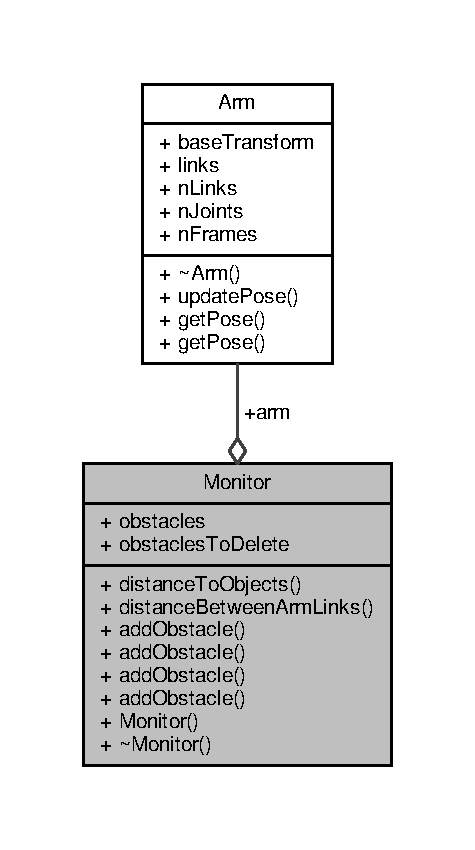
\includegraphics[height=550pt]{class_monitor__coll__graph}
\end{center}
\end{figure}
\subsection*{Public Member Functions}
\begin{DoxyCompactItemize}
\item 
std\+::vector$<$ std\+::vector$<$ double $>$ $>$ \hyperlink{class_monitor_a1801675787693435342ae799975b1120}{distance\+To\+Objects} ()
\item 
std\+::vector$<$ double $>$ \hyperlink{class_monitor_a1e4ef4f45f75dcc38d6283644a4bfdbe}{base\+Distance\+To\+Objects} ()
\item 
std\+::vector$<$ std\+::vector$<$ double $>$ $>$ \hyperlink{class_monitor_afe72152adc0d2d2faf8fb01563417033}{distance\+Between\+Arm\+Links} ()
\item 
void \hyperlink{class_monitor_a8c448bcff703af93489cc4f0847d4245}{add\+Obstacle} (\hyperlink{class_primitive}{Primitive} $\ast$obstacle)
\item 
void \hyperlink{class_monitor_af5979d8f05c2d945ddc055e329fad5d2}{add\+Obstacle} (\hyperlink{class_sphere}{Sphere} $\ast$obstacle)
\item 
void \hyperlink{class_monitor_a192497730489ebcd6a6580875cfbeee3}{add\+Obstacle} (\hyperlink{class_capsule}{Capsule} $\ast$obstacle)
\item 
void \hyperlink{class_monitor_a580dedf3090ffff7a452dbe32cc585f4}{add\+Obstacle} (\hyperlink{class_arm}{Arm} $\ast$\hyperlink{class_monitor_a8b75571f6224f999a3dc05cf9a83fa68}{arm})
\item 
void \hyperlink{class_monitor_ada0a962c56c54acb79a900dd9ef555b6}{add\+Obstacle} (\hyperlink{class_base}{Base} $\ast$base\+\_\+obstacle)
\item 
void \hyperlink{class_monitor_aa4f85c0ea9c00b1d633f69fa5ffef4cd}{add\+Obstacle} (\hyperlink{class_box3}{Box3} $\ast$box)
\item 
\hyperlink{class_monitor_a0761228d7a5ca8c0e272e5e3bec5bef8}{Monitor} (\hyperlink{class_base}{Base} $\ast$\hyperlink{class_monitor_a62aac32130c77d66f9cec4a06d5e75a7}{base})
\item 
\hyperlink{class_monitor_adda7d547e1226e159836356dd8af14bb}{Monitor} (\hyperlink{class_arm}{Arm} $\ast$\hyperlink{class_monitor_a8b75571f6224f999a3dc05cf9a83fa68}{arm})
\item 
\hyperlink{class_monitor_a64aba8195effc068092ddea5a71e8176}{$\sim$\+Monitor} ()
\end{DoxyCompactItemize}
\subsection*{Public Attributes}
\begin{DoxyCompactItemize}
\item 
\hyperlink{class_arm}{Arm} $\ast$ \hyperlink{class_monitor_a8b75571f6224f999a3dc05cf9a83fa68}{arm}
\begin{DoxyCompactList}\small\item\em \hyperlink{class_arm}{Arm} for the monitor. \end{DoxyCompactList}\item 
\hyperlink{class_base}{Base} $\ast$ \hyperlink{class_monitor_a62aac32130c77d66f9cec4a06d5e75a7}{base}
\item 
std\+::vector$<$ \hyperlink{class_primitive}{Primitive} $\ast$ $>$ \hyperlink{class_monitor_a05fd42482269ad65432d5400c8f0f9b5}{obstacles}
\begin{DoxyCompactList}\small\item\em Obstacles in the workspace. \end{DoxyCompactList}\item 
std\+::vector$<$ \hyperlink{class_primitive}{Primitive} $\ast$ $>$ \hyperlink{class_monitor_a2207169c2b32b3bbf9925f3254064dee}{obstacles\+To\+Delete}
\begin{DoxyCompactList}\small\item\em Obstacles to delete in destructor. \end{DoxyCompactList}\end{DoxyCompactItemize}


\subsection{Detailed Description}
A collision monitor to determine the distance to obstacles and other links

The \hyperlink{class_monitor}{Monitor} class is a collision monitor which stores the address of an instance of the class \hyperlink{class_arm}{Arm} and maintains a list of obstacles. It can perform collision monitoring with obstacles by determining the distance to obstacles in the workspace, or collision monitoring with the arm itself by monitoring the distance between the links. 

\subsection{Constructor \& Destructor Documentation}
\index{Monitor@{Monitor}!Monitor@{Monitor}}
\index{Monitor@{Monitor}!Monitor@{Monitor}}
\subsubsection[{\texorpdfstring{Monitor(\+Base $\ast$base)}{Monitor(Base *base)}}]{\setlength{\rightskip}{0pt plus 5cm}Monitor\+::\+Monitor (
\begin{DoxyParamCaption}
\item[{{\bf Base} $\ast$}]{base}
\end{DoxyParamCaption}
)}\hypertarget{class_monitor_a0761228d7a5ca8c0e272e5e3bec5bef8}{}\label{class_monitor_a0761228d7a5ca8c0e272e5e3bec5bef8}
Constructor of \hyperlink{class_monitor}{Monitor}

This is the constructor for the monitor class, it takes as paramter the arm to be monitored.


\begin{DoxyParams}{Parameters}
{\em arm} & arm to monitor collision.\+Constructor of \hyperlink{class_monitor}{Monitor} \begin{DoxyVerb}This is the constructor for the monitor class, it takes as 
paramter the base to be monitored. 

@param base base to monitor collision.\end{DoxyVerb}
 \\
\hline
\end{DoxyParams}
\index{Monitor@{Monitor}!Monitor@{Monitor}}
\index{Monitor@{Monitor}!Monitor@{Monitor}}
\subsubsection[{\texorpdfstring{Monitor(\+Arm $\ast$arm)}{Monitor(Arm *arm)}}]{\setlength{\rightskip}{0pt plus 5cm}Monitor\+::\+Monitor (
\begin{DoxyParamCaption}
\item[{{\bf Arm} $\ast$}]{arm}
\end{DoxyParamCaption}
)}\hypertarget{class_monitor_adda7d547e1226e159836356dd8af14bb}{}\label{class_monitor_adda7d547e1226e159836356dd8af14bb}
\index{Monitor@{Monitor}!````~Monitor@{$\sim$\+Monitor}}
\index{````~Monitor@{$\sim$\+Monitor}!Monitor@{Monitor}}
\subsubsection[{\texorpdfstring{$\sim$\+Monitor()}{~Monitor()}}]{\setlength{\rightskip}{0pt plus 5cm}Monitor\+::$\sim$\+Monitor (
\begin{DoxyParamCaption}
{}
\end{DoxyParamCaption}
)}\hypertarget{class_monitor_a64aba8195effc068092ddea5a71e8176}{}\label{class_monitor_a64aba8195effc068092ddea5a71e8176}
Destructor for the monitor class 

\subsection{Member Function Documentation}
\index{Monitor@{Monitor}!add\+Obstacle@{add\+Obstacle}}
\index{add\+Obstacle@{add\+Obstacle}!Monitor@{Monitor}}
\subsubsection[{\texorpdfstring{add\+Obstacle(\+Primitive $\ast$obstacle)}{addObstacle(Primitive *obstacle)}}]{\setlength{\rightskip}{0pt plus 5cm}void Monitor\+::add\+Obstacle (
\begin{DoxyParamCaption}
\item[{{\bf Primitive} $\ast$}]{obstacle}
\end{DoxyParamCaption}
)}\hypertarget{class_monitor_a8c448bcff703af93489cc4f0847d4245}{}\label{class_monitor_a8c448bcff703af93489cc4f0847d4245}
Adds primitive to list of obstacles

Adds a primitive to the list of obstacles. 
\begin{DoxyParams}{Parameters}
{\em obstacle} & address of the obstacle to be added. \\
\hline
\end{DoxyParams}
\index{Monitor@{Monitor}!add\+Obstacle@{add\+Obstacle}}
\index{add\+Obstacle@{add\+Obstacle}!Monitor@{Monitor}}
\subsubsection[{\texorpdfstring{add\+Obstacle(\+Sphere $\ast$obstacle)}{addObstacle(Sphere *obstacle)}}]{\setlength{\rightskip}{0pt plus 5cm}void Monitor\+::add\+Obstacle (
\begin{DoxyParamCaption}
\item[{{\bf Sphere} $\ast$}]{obstacle}
\end{DoxyParamCaption}
)}\hypertarget{class_monitor_af5979d8f05c2d945ddc055e329fad5d2}{}\label{class_monitor_af5979d8f05c2d945ddc055e329fad5d2}
Adds primitive to list of obstacles

Adds a primitive to the list of obstacles. 
\begin{DoxyParams}{Parameters}
{\em obstacle} & address of the obstacle to be added. \\
\hline
\end{DoxyParams}
\index{Monitor@{Monitor}!add\+Obstacle@{add\+Obstacle}}
\index{add\+Obstacle@{add\+Obstacle}!Monitor@{Monitor}}
\subsubsection[{\texorpdfstring{add\+Obstacle(\+Capsule $\ast$obstacle)}{addObstacle(Capsule *obstacle)}}]{\setlength{\rightskip}{0pt plus 5cm}void Monitor\+::add\+Obstacle (
\begin{DoxyParamCaption}
\item[{{\bf Capsule} $\ast$}]{obstacle}
\end{DoxyParamCaption}
)}\hypertarget{class_monitor_a192497730489ebcd6a6580875cfbeee3}{}\label{class_monitor_a192497730489ebcd6a6580875cfbeee3}
Adds primitive to list of obstacles

Adds a primitive to the list of obstacles. 
\begin{DoxyParams}{Parameters}
{\em obstacle} & address of the obstacle to be added. \\
\hline
\end{DoxyParams}
\index{Monitor@{Monitor}!add\+Obstacle@{add\+Obstacle}}
\index{add\+Obstacle@{add\+Obstacle}!Monitor@{Monitor}}
\subsubsection[{\texorpdfstring{add\+Obstacle(\+Arm $\ast$arm)}{addObstacle(Arm *arm)}}]{\setlength{\rightskip}{0pt plus 5cm}void Monitor\+::add\+Obstacle (
\begin{DoxyParamCaption}
\item[{{\bf Arm} $\ast$}]{arm}
\end{DoxyParamCaption}
)}\hypertarget{class_monitor_a580dedf3090ffff7a452dbe32cc585f4}{}\label{class_monitor_a580dedf3090ffff7a452dbe32cc585f4}
Adds arm to list of obstacles

This method decomposes an arm into its primitives to add it into the vector of obstacles.


\begin{DoxyParams}{Parameters}
{\em arm} & address of the arm to be treated as an obstacle. \\
\hline
\end{DoxyParams}
\index{Monitor@{Monitor}!add\+Obstacle@{add\+Obstacle}}
\index{add\+Obstacle@{add\+Obstacle}!Monitor@{Monitor}}
\subsubsection[{\texorpdfstring{add\+Obstacle(\+Base $\ast$base\+\_\+obstacle)}{addObstacle(Base *base_obstacle)}}]{\setlength{\rightskip}{0pt plus 5cm}void Monitor\+::add\+Obstacle (
\begin{DoxyParamCaption}
\item[{{\bf Base} $\ast$}]{base\+\_\+obstacle}
\end{DoxyParamCaption}
)}\hypertarget{class_monitor_ada0a962c56c54acb79a900dd9ef555b6}{}\label{class_monitor_ada0a962c56c54acb79a900dd9ef555b6}
Adds base to list of obstacles

This method decomposes a base into its box3 primitive to add it into the vector of obstacles.


\begin{DoxyParams}{Parameters}
{\em base} & address of the base to be treated as an obstacle. \\
\hline
\end{DoxyParams}
\index{Monitor@{Monitor}!add\+Obstacle@{add\+Obstacle}}
\index{add\+Obstacle@{add\+Obstacle}!Monitor@{Monitor}}
\subsubsection[{\texorpdfstring{add\+Obstacle(\+Box3 $\ast$box)}{addObstacle(Box3 *box)}}]{\setlength{\rightskip}{0pt plus 5cm}void Monitor\+::add\+Obstacle (
\begin{DoxyParamCaption}
\item[{{\bf Box3} $\ast$}]{box}
\end{DoxyParamCaption}
)}\hypertarget{class_monitor_aa4f85c0ea9c00b1d633f69fa5ffef4cd}{}\label{class_monitor_aa4f85c0ea9c00b1d633f69fa5ffef4cd}
Adds box to list of obstacles

Adds a box to the list of obstacles. 
\begin{DoxyParams}{Parameters}
{\em box} & address of the box obstacle to be added. \\
\hline
\end{DoxyParams}
\index{Monitor@{Monitor}!base\+Distance\+To\+Objects@{base\+Distance\+To\+Objects}}
\index{base\+Distance\+To\+Objects@{base\+Distance\+To\+Objects}!Monitor@{Monitor}}
\subsubsection[{\texorpdfstring{base\+Distance\+To\+Objects()}{baseDistanceToObjects()}}]{\setlength{\rightskip}{0pt plus 5cm}std\+::vector$<$ double $>$ Monitor\+::base\+Distance\+To\+Objects (
\begin{DoxyParamCaption}
{}
\end{DoxyParamCaption}
)}\hypertarget{class_monitor_a1e4ef4f45f75dcc38d6283644a4bfdbe}{}\label{class_monitor_a1e4ef4f45f75dcc38d6283644a4bfdbe}
Collision monitoring with the base and other obstacles.

This methods monitors the distance from base of the robot to other obstacles.

\begin{DoxyReturn}{Returns}
a matrix with the distance of each link to the other links. 
\end{DoxyReturn}
\index{Monitor@{Monitor}!distance\+Between\+Arm\+Links@{distance\+Between\+Arm\+Links}}
\index{distance\+Between\+Arm\+Links@{distance\+Between\+Arm\+Links}!Monitor@{Monitor}}
\subsubsection[{\texorpdfstring{distance\+Between\+Arm\+Links()}{distanceBetweenArmLinks()}}]{\setlength{\rightskip}{0pt plus 5cm}std\+::vector$<$ std\+::vector$<$ double $>$ $>$ Monitor\+::distance\+Between\+Arm\+Links (
\begin{DoxyParamCaption}
{}
\end{DoxyParamCaption}
)}\hypertarget{class_monitor_afe72152adc0d2d2faf8fb01563417033}{}\label{class_monitor_afe72152adc0d2d2faf8fb01563417033}
Collision monitoring with the arm itself.

This methods monitors the distance from one link of the arm to other links.

\begin{DoxyReturn}{Returns}
a matrix with the distance of each link to the other links. 
\end{DoxyReturn}
\index{Monitor@{Monitor}!distance\+To\+Objects@{distance\+To\+Objects}}
\index{distance\+To\+Objects@{distance\+To\+Objects}!Monitor@{Monitor}}
\subsubsection[{\texorpdfstring{distance\+To\+Objects()}{distanceToObjects()}}]{\setlength{\rightskip}{0pt plus 5cm}std\+::vector$<$ std\+::vector$<$ double $>$ $>$ Monitor\+::distance\+To\+Objects (
\begin{DoxyParamCaption}
{}
\end{DoxyParamCaption}
)}\hypertarget{class_monitor_a1801675787693435342ae799975b1120}{}\label{class_monitor_a1801675787693435342ae799975b1120}
Collision monitoring with obstacles.

This methods monitors the distance from one link of the arm to obstacles in the workspace.

\begin{DoxyReturn}{Returns}
a matrix with the distance of each link to the other obstacles. 
\end{DoxyReturn}


\subsection{Member Data Documentation}
\index{Monitor@{Monitor}!arm@{arm}}
\index{arm@{arm}!Monitor@{Monitor}}
\subsubsection[{\texorpdfstring{arm}{arm}}]{\setlength{\rightskip}{0pt plus 5cm}{\bf Arm}$\ast$ Monitor\+::arm}\hypertarget{class_monitor_a8b75571f6224f999a3dc05cf9a83fa68}{}\label{class_monitor_a8b75571f6224f999a3dc05cf9a83fa68}


\hyperlink{class_arm}{Arm} for the monitor. 

\index{Monitor@{Monitor}!base@{base}}
\index{base@{base}!Monitor@{Monitor}}
\subsubsection[{\texorpdfstring{base}{base}}]{\setlength{\rightskip}{0pt plus 5cm}{\bf Base}$\ast$ Monitor\+::base}\hypertarget{class_monitor_a62aac32130c77d66f9cec4a06d5e75a7}{}\label{class_monitor_a62aac32130c77d66f9cec4a06d5e75a7}
\index{Monitor@{Monitor}!obstacles@{obstacles}}
\index{obstacles@{obstacles}!Monitor@{Monitor}}
\subsubsection[{\texorpdfstring{obstacles}{obstacles}}]{\setlength{\rightskip}{0pt plus 5cm}std\+::vector$<${\bf Primitive}$\ast$$>$ Monitor\+::obstacles}\hypertarget{class_monitor_a05fd42482269ad65432d5400c8f0f9b5}{}\label{class_monitor_a05fd42482269ad65432d5400c8f0f9b5}


Obstacles in the workspace. 

\index{Monitor@{Monitor}!obstacles\+To\+Delete@{obstacles\+To\+Delete}}
\index{obstacles\+To\+Delete@{obstacles\+To\+Delete}!Monitor@{Monitor}}
\subsubsection[{\texorpdfstring{obstacles\+To\+Delete}{obstaclesToDelete}}]{\setlength{\rightskip}{0pt plus 5cm}std\+::vector$<${\bf Primitive}$\ast$$>$ Monitor\+::obstacles\+To\+Delete}\hypertarget{class_monitor_a2207169c2b32b3bbf9925f3254064dee}{}\label{class_monitor_a2207169c2b32b3bbf9925f3254064dee}


Obstacles to delete in destructor. 



The documentation for this class was generated from the following files\+:\begin{DoxyCompactItemize}
\item 
/home/srini/hbrs/\+Fourthsem/\+S\+D\+P/\+R\+O\+S\+\_\+setup/08032021/updated\+\_\+1/sdp\+\_\+ws20\+\_\+collision\+\_\+monitoring\+\_\+for\+\_\+mobile\+\_\+manipulators/collision\+\_\+monitoring/include/\hyperlink{monitor_8h}{monitor.\+h}\item 
/home/srini/hbrs/\+Fourthsem/\+S\+D\+P/\+R\+O\+S\+\_\+setup/08032021/updated\+\_\+1/sdp\+\_\+ws20\+\_\+collision\+\_\+monitoring\+\_\+for\+\_\+mobile\+\_\+manipulators/collision\+\_\+monitoring/src/\hyperlink{monitor_8cpp}{monitor.\+cpp}\end{DoxyCompactItemize}

\hypertarget{class_primitive}{}\section{Primitive Class Reference}
\label{class_primitive}\index{Primitive@{Primitive}}


{\ttfamily \#include $<$primitives.\+h$>$}



Inheritance diagram for Primitive\+:
\nopagebreak
\begin{figure}[H]
\begin{center}
\leavevmode
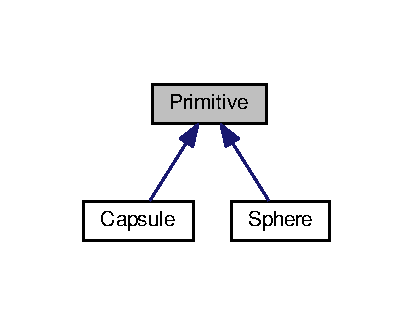
\includegraphics[width=340pt]{class_primitive__inherit__graph}
\end{center}
\end{figure}


Collaboration diagram for Primitive\+:
\nopagebreak
\begin{figure}[H]
\begin{center}
\leavevmode
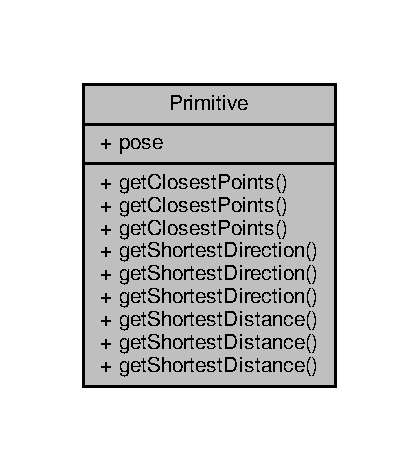
\includegraphics[width=201pt]{class_primitive__coll__graph}
\end{center}
\end{figure}
\subsection*{Public Member Functions}
\begin{DoxyCompactItemize}
\item 
virtual void \hyperlink{class_primitive_ae838e4e129f05642994da59f08f85f56}{get\+Closest\+Points} (Eigen\+::\+Matrix\+Xd \&closest\+Points, \hyperlink{class_primitive}{Primitive} $\ast$primitive)=0
\item 
virtual void \hyperlink{class_primitive_a2b8b8dea111d9eda31f72e06b47e9aa9}{get\+Closest\+Points} (Eigen\+::\+Matrix\+Xd \&closest\+Points, \hyperlink{class_capsule}{Capsule} $\ast$capsule)=0
\item 
virtual void \hyperlink{class_primitive_ac86ef47d59c21448ce78c91490c7dbd4}{get\+Closest\+Points} (Eigen\+::\+Matrix\+Xd \&closest\+Points, \hyperlink{class_sphere}{Sphere} $\ast$sphere)=0
\item 
virtual void \hyperlink{class_primitive_ae37bbdf5271bf278b19888e0428579a8}{get\+Shortest\+Direction} (Eigen\+::\+Vector3d \&shortest\+Direction, \hyperlink{class_primitive}{Primitive} $\ast$primitive)=0
\item 
virtual void \hyperlink{class_primitive_af9bd724a6618bd76e41e5682caa25023}{get\+Shortest\+Direction} (Eigen\+::\+Vector3d \&shortest\+Direction, \hyperlink{class_capsule}{Capsule} $\ast$capsule)=0
\item 
virtual void \hyperlink{class_primitive_a3f1bc91de29fa904657c1ba4c40eee53}{get\+Shortest\+Direction} (Eigen\+::\+Vector3d \&shortest\+Direction, \hyperlink{class_sphere}{Sphere} $\ast$sphere)=0
\item 
virtual double \hyperlink{class_primitive_a340b3e5540b910480ada939383985d66}{get\+Shortest\+Distance} (\hyperlink{class_primitive}{Primitive} $\ast$primitive)=0
\item 
virtual double \hyperlink{class_primitive_a46e60acfe4c005c0ec94e1e8b82d36db}{get\+Shortest\+Distance} (\hyperlink{class_capsule}{Capsule} $\ast$capsule)=0
\item 
virtual double \hyperlink{class_primitive_adaac4fc4fedf9cd76d4eb9c77e9ae560}{get\+Shortest\+Distance} (\hyperlink{class_sphere}{Sphere} $\ast$sphere)=0
\end{DoxyCompactItemize}
\subsection*{Public Attributes}
\begin{DoxyCompactItemize}
\item 
Eigen\+::\+Matrix4d \hyperlink{class_primitive_ad8b2afbad412f6046783d155c88fe312}{pose}
\end{DoxyCompactItemize}


\subsection{Detailed Description}
An abstract class that contains the basic attributes of all primitives

This abstract class gets inherited by all primitive shapes. All shapes have a pose expressed by a Eigen Matrix4d, and a family of methods to get the shortest distrance from this primitive to another one depending the class of the latter. 

Definition at line 30 of file primitives.\+h.



\subsection{Member Function Documentation}
\index{Primitive@{Primitive}!get\+Closest\+Points@{get\+Closest\+Points}}
\index{get\+Closest\+Points@{get\+Closest\+Points}!Primitive@{Primitive}}
\subsubsection[{\texorpdfstring{get\+Closest\+Points(\+Eigen\+::\+Matrix\+Xd \&closest\+Points, Primitive $\ast$primitive)=0}{getClosestPoints(Eigen::MatrixXd &closestPoints, Primitive *primitive)=0}}]{\setlength{\rightskip}{0pt plus 5cm}virtual void Primitive\+::get\+Closest\+Points (
\begin{DoxyParamCaption}
\item[{Eigen\+::\+Matrix\+Xd \&}]{closest\+Points, }
\item[{{\bf Primitive} $\ast$}]{primitive}
\end{DoxyParamCaption}
)\hspace{0.3cm}{\ttfamily [pure virtual]}}\hypertarget{class_primitive_ae838e4e129f05642994da59f08f85f56}{}\label{class_primitive_ae838e4e129f05642994da59f08f85f56}
Performs a dynamic cast to overload the direction functions

This method takes an object that inherits from primitive and performs a dynamic cast to call the correct get\+Closest\+Points method depending on the class of the shape.


\begin{DoxyParams}[1]{Parameters}
 & {\em primitive} & address of the primitive object. \\
\hline
\mbox{\tt out}  & {\em closest\+Points} & the closest points in this primitive and primitive \\
\hline
\end{DoxyParams}


Implemented in \hyperlink{class_sphere_a9290773136dacf81a9f147343a7a0486}{Sphere}, and \hyperlink{class_capsule_aec53e0cf5f8644f1413c3c208de64cc7}{Capsule}.

\index{Primitive@{Primitive}!get\+Closest\+Points@{get\+Closest\+Points}}
\index{get\+Closest\+Points@{get\+Closest\+Points}!Primitive@{Primitive}}
\subsubsection[{\texorpdfstring{get\+Closest\+Points(\+Eigen\+::\+Matrix\+Xd \&closest\+Points, Capsule $\ast$capsule)=0}{getClosestPoints(Eigen::MatrixXd &closestPoints, Capsule *capsule)=0}}]{\setlength{\rightskip}{0pt plus 5cm}virtual void Primitive\+::get\+Closest\+Points (
\begin{DoxyParamCaption}
\item[{Eigen\+::\+Matrix\+Xd \&}]{closest\+Points, }
\item[{{\bf Capsule} $\ast$}]{capsule}
\end{DoxyParamCaption}
)\hspace{0.3cm}{\ttfamily [pure virtual]}}\hypertarget{class_primitive_a2b8b8dea111d9eda31f72e06b47e9aa9}{}\label{class_primitive_a2b8b8dea111d9eda31f72e06b47e9aa9}
Finds the shortest distance between this primitive and a \hyperlink{class_capsule}{Capsule} primitive

This method takes a capsule object and returns the closest points in this primitive and in a capsule object.


\begin{DoxyParams}[1]{Parameters}
 & {\em capsule} & address of the primitive object \\
\hline
\mbox{\tt out}  & {\em closest\+Points} & the closest points in this primitive and capsule \\
\hline
\end{DoxyParams}


Implemented in \hyperlink{class_sphere_a903c1c7a459e0c048b6f36a4f1376256}{Sphere}, and \hyperlink{class_capsule_a9da1b4c44adba1726446a4fb37b7a7e0}{Capsule}.

\index{Primitive@{Primitive}!get\+Closest\+Points@{get\+Closest\+Points}}
\index{get\+Closest\+Points@{get\+Closest\+Points}!Primitive@{Primitive}}
\subsubsection[{\texorpdfstring{get\+Closest\+Points(\+Eigen\+::\+Matrix\+Xd \&closest\+Points, Sphere $\ast$sphere)=0}{getClosestPoints(Eigen::MatrixXd &closestPoints, Sphere *sphere)=0}}]{\setlength{\rightskip}{0pt plus 5cm}virtual void Primitive\+::get\+Closest\+Points (
\begin{DoxyParamCaption}
\item[{Eigen\+::\+Matrix\+Xd \&}]{closest\+Points, }
\item[{{\bf Sphere} $\ast$}]{sphere}
\end{DoxyParamCaption}
)\hspace{0.3cm}{\ttfamily [pure virtual]}}\hypertarget{class_primitive_ac86ef47d59c21448ce78c91490c7dbd4}{}\label{class_primitive_ac86ef47d59c21448ce78c91490c7dbd4}
Finds the shortest distance between this primitive and a \hyperlink{class_sphere}{Sphere} primitive

This method takes a capsule object and returns the closest points in this primitive and in a sphere object.


\begin{DoxyParams}[1]{Parameters}
 & {\em sphere} & address of the primitive object \\
\hline
\mbox{\tt out}  & {\em closest\+Points} & the closest points in this primitive and sphere \\
\hline
\end{DoxyParams}


Implemented in \hyperlink{class_sphere_ac2584cb5fb1d066a9527f8c95435093b}{Sphere}, and \hyperlink{class_capsule_aa0fea610bb1a1e4016bbda0f4f88264a}{Capsule}.

\index{Primitive@{Primitive}!get\+Shortest\+Direction@{get\+Shortest\+Direction}}
\index{get\+Shortest\+Direction@{get\+Shortest\+Direction}!Primitive@{Primitive}}
\subsubsection[{\texorpdfstring{get\+Shortest\+Direction(\+Eigen\+::\+Vector3d \&shortest\+Direction, Primitive $\ast$primitive)=0}{getShortestDirection(Eigen::Vector3d &shortestDirection, Primitive *primitive)=0}}]{\setlength{\rightskip}{0pt plus 5cm}virtual void Primitive\+::get\+Shortest\+Direction (
\begin{DoxyParamCaption}
\item[{Eigen\+::\+Vector3d \&}]{shortest\+Direction, }
\item[{{\bf Primitive} $\ast$}]{primitive}
\end{DoxyParamCaption}
)\hspace{0.3cm}{\ttfamily [pure virtual]}}\hypertarget{class_primitive_ae37bbdf5271bf278b19888e0428579a8}{}\label{class_primitive_ae37bbdf5271bf278b19888e0428579a8}
Performs a dynamic cast to overload the direction functions

This method takes an object that inherits from primitive and performs a dynamic cast to call the correct get\+Shortest\+Direction method depending on the class of the shape.


\begin{DoxyParams}[1]{Parameters}
 & {\em primitive} & address of the primitive object. \\
\hline
\mbox{\tt out}  & {\em shortest\+Direction} & a vector in 3D that represents the closes direction between this and the second primitive. \\
\hline
\end{DoxyParams}


Implemented in \hyperlink{class_sphere_a707fc14e03a6ff67ac012a18b2a8cb28}{Sphere}, and \hyperlink{class_capsule_ad569eae23b91f33e145f06745739e428}{Capsule}.

\index{Primitive@{Primitive}!get\+Shortest\+Direction@{get\+Shortest\+Direction}}
\index{get\+Shortest\+Direction@{get\+Shortest\+Direction}!Primitive@{Primitive}}
\subsubsection[{\texorpdfstring{get\+Shortest\+Direction(\+Eigen\+::\+Vector3d \&shortest\+Direction, Capsule $\ast$capsule)=0}{getShortestDirection(Eigen::Vector3d &shortestDirection, Capsule *capsule)=0}}]{\setlength{\rightskip}{0pt plus 5cm}virtual void Primitive\+::get\+Shortest\+Direction (
\begin{DoxyParamCaption}
\item[{Eigen\+::\+Vector3d \&}]{shortest\+Direction, }
\item[{{\bf Capsule} $\ast$}]{capsule}
\end{DoxyParamCaption}
)\hspace{0.3cm}{\ttfamily [pure virtual]}}\hypertarget{class_primitive_af9bd724a6618bd76e41e5682caa25023}{}\label{class_primitive_af9bd724a6618bd76e41e5682caa25023}
Finds the shortest distance between this primitive and a \hyperlink{class_capsule}{Capsule} primitive

This method takes a capsule object and returns the closest direction between this primitive and a capsule object.


\begin{DoxyParams}[1]{Parameters}
 & {\em capsule} & address of the primitive object \\
\hline
\mbox{\tt out}  & {\em shortest\+Direction} & a vector in 3D that represents the closes direction between the primitive and capsule \\
\hline
\end{DoxyParams}


Implemented in \hyperlink{class_sphere_af7ff30023363261cf118d1fb80c745a7}{Sphere}, and \hyperlink{class_capsule_a28274c18ef5a3b9ef869caa64d5f7d5e}{Capsule}.

\index{Primitive@{Primitive}!get\+Shortest\+Direction@{get\+Shortest\+Direction}}
\index{get\+Shortest\+Direction@{get\+Shortest\+Direction}!Primitive@{Primitive}}
\subsubsection[{\texorpdfstring{get\+Shortest\+Direction(\+Eigen\+::\+Vector3d \&shortest\+Direction, Sphere $\ast$sphere)=0}{getShortestDirection(Eigen::Vector3d &shortestDirection, Sphere *sphere)=0}}]{\setlength{\rightskip}{0pt plus 5cm}virtual void Primitive\+::get\+Shortest\+Direction (
\begin{DoxyParamCaption}
\item[{Eigen\+::\+Vector3d \&}]{shortest\+Direction, }
\item[{{\bf Sphere} $\ast$}]{sphere}
\end{DoxyParamCaption}
)\hspace{0.3cm}{\ttfamily [pure virtual]}}\hypertarget{class_primitive_a3f1bc91de29fa904657c1ba4c40eee53}{}\label{class_primitive_a3f1bc91de29fa904657c1ba4c40eee53}
Finds the shortest distance between this primitive and a \hyperlink{class_sphere}{Sphere} primitive

This method takes a capsule object and returns the closest direction between this primitive and a sphere object.


\begin{DoxyParams}[1]{Parameters}
 & {\em sphere} & address of the primitive object \\
\hline
\mbox{\tt out}  & {\em shortest\+Direction} & a vector in 3D that represents the closes direction between the primitive and sphere \\
\hline
\end{DoxyParams}


Implemented in \hyperlink{class_sphere_a719592bc6a8307060f49f289da631310}{Sphere}, and \hyperlink{class_capsule_aae076a389170bd6644f479bfe9c243bc}{Capsule}.

\index{Primitive@{Primitive}!get\+Shortest\+Distance@{get\+Shortest\+Distance}}
\index{get\+Shortest\+Distance@{get\+Shortest\+Distance}!Primitive@{Primitive}}
\subsubsection[{\texorpdfstring{get\+Shortest\+Distance(\+Primitive $\ast$primitive)=0}{getShortestDistance(Primitive *primitive)=0}}]{\setlength{\rightskip}{0pt plus 5cm}virtual double Primitive\+::get\+Shortest\+Distance (
\begin{DoxyParamCaption}
\item[{{\bf Primitive} $\ast$}]{primitive}
\end{DoxyParamCaption}
)\hspace{0.3cm}{\ttfamily [pure virtual]}}\hypertarget{class_primitive_a340b3e5540b910480ada939383985d66}{}\label{class_primitive_a340b3e5540b910480ada939383985d66}
Performs a dynamic cast to overload the distance functions

This method takes an object that inherits from primitive and performs a dynamic cast to call the correct get\+Shortest\+Distance method depending on the class of the shape. returns a double value.


\begin{DoxyParams}{Parameters}
{\em primitive} & address of the primitive object. \\
\hline
\end{DoxyParams}
\begin{DoxyReturn}{Returns}
the closest distance between this and the second primitive. 
\end{DoxyReturn}


Implemented in \hyperlink{class_sphere_a7330816427e4099f4a8ccb8c34bd9ec6}{Sphere}, and \hyperlink{class_capsule_a43bcc7bb95425a4559f7fd0289ef8b45}{Capsule}.

\index{Primitive@{Primitive}!get\+Shortest\+Distance@{get\+Shortest\+Distance}}
\index{get\+Shortest\+Distance@{get\+Shortest\+Distance}!Primitive@{Primitive}}
\subsubsection[{\texorpdfstring{get\+Shortest\+Distance(\+Capsule $\ast$capsule)=0}{getShortestDistance(Capsule *capsule)=0}}]{\setlength{\rightskip}{0pt plus 5cm}virtual double Primitive\+::get\+Shortest\+Distance (
\begin{DoxyParamCaption}
\item[{{\bf Capsule} $\ast$}]{capsule}
\end{DoxyParamCaption}
)\hspace{0.3cm}{\ttfamily [pure virtual]}}\hypertarget{class_primitive_a46e60acfe4c005c0ec94e1e8b82d36db}{}\label{class_primitive_a46e60acfe4c005c0ec94e1e8b82d36db}
Finds the shortest distance between this primitive and a \hyperlink{class_capsule}{Capsule} primitive

This method takes a capsule object and returns the closest distance between this primitive and a capsule object. returns a double value.


\begin{DoxyParams}{Parameters}
{\em capsule} & address of the primitive object \\
\hline
\end{DoxyParams}
\begin{DoxyReturn}{Returns}
the closest distance between the primitive and capsule 
\end{DoxyReturn}


Implemented in \hyperlink{class_sphere_a2b078585c4b272e9286eac12189b885b}{Sphere}, and \hyperlink{class_capsule_ade8880442a9230f893c296f0681ae9ad}{Capsule}.

\index{Primitive@{Primitive}!get\+Shortest\+Distance@{get\+Shortest\+Distance}}
\index{get\+Shortest\+Distance@{get\+Shortest\+Distance}!Primitive@{Primitive}}
\subsubsection[{\texorpdfstring{get\+Shortest\+Distance(\+Sphere $\ast$sphere)=0}{getShortestDistance(Sphere *sphere)=0}}]{\setlength{\rightskip}{0pt plus 5cm}virtual double Primitive\+::get\+Shortest\+Distance (
\begin{DoxyParamCaption}
\item[{{\bf Sphere} $\ast$}]{sphere}
\end{DoxyParamCaption}
)\hspace{0.3cm}{\ttfamily [pure virtual]}}\hypertarget{class_primitive_adaac4fc4fedf9cd76d4eb9c77e9ae560}{}\label{class_primitive_adaac4fc4fedf9cd76d4eb9c77e9ae560}
Finds the shortest distance between this primitive and a \hyperlink{class_sphere}{Sphere} primitive

This method takes a capsule object and returns the closest distance between this primitive and a sphere object. returns a double value.


\begin{DoxyParams}{Parameters}
{\em sphere} & address of the primitive object \\
\hline
\end{DoxyParams}
\begin{DoxyReturn}{Returns}
the closest distance between the primitive and sphere 
\end{DoxyReturn}


Implemented in \hyperlink{class_sphere_a6efb9b513c9b42a7b040969b802727ea}{Sphere}, and \hyperlink{class_capsule_a71d7821f3e7f9ac972bceb06d82f529d}{Capsule}.



\subsection{Member Data Documentation}
\index{Primitive@{Primitive}!pose@{pose}}
\index{pose@{pose}!Primitive@{Primitive}}
\subsubsection[{\texorpdfstring{pose}{pose}}]{\setlength{\rightskip}{0pt plus 5cm}Eigen\+::\+Matrix4d Primitive\+::pose}\hypertarget{class_primitive_ad8b2afbad412f6046783d155c88fe312}{}\label{class_primitive_ad8b2afbad412f6046783d155c88fe312}
Finds the shortest distance between this primitive and a Cylinder primitive

This method takes a capsule object and returns the closest distance between this primitive and a cylinder object. returns a double value.


\begin{DoxyParams}{Parameters}
{\em cylinder} & address of the primitive object \\
\hline
\end{DoxyParams}
\begin{DoxyReturn}{Returns}
the closest distance between the primitive and cylinder 
\end{DoxyReturn}


Definition at line 138 of file primitives.\+h.



The documentation for this class was generated from the following file\+:\begin{DoxyCompactItemize}
\item 
\hyperlink{primitives_8h}{primitives.\+h}\end{DoxyCompactItemize}

\hypertarget{class_rviz_obstacle}{}\section{Rviz\+Obstacle Class Reference}
\label{class_rviz_obstacle}\index{Rviz\+Obstacle@{Rviz\+Obstacle}}
\subsection*{Public Member Functions}
\begin{DoxyCompactItemize}
\item 
{\bfseries Rviz\+Obstacle} (visualization\+\_\+msgs\+::\+Marker\+::\+Const\+Ptr marker\+In, int index)\hypertarget{class_rviz_obstacle_a3fb19f60434581b669c0dc063c026943}{}\label{class_rviz_obstacle_a3fb19f60434581b669c0dc063c026943}

\item 
Eigen\+::\+Matrix4d {\bfseries update\+Pose} (visualization\+\_\+msgs\+::\+Marker\+::\+Const\+Ptr marker\+In)\hypertarget{class_rviz_obstacle_a30101e2a3c65776bb4abbb139f10b14a}{}\label{class_rviz_obstacle_a30101e2a3c65776bb4abbb139f10b14a}

\end{DoxyCompactItemize}
\subsection*{Public Attributes}
\begin{DoxyCompactItemize}
\item 
int {\bfseries idx}\hypertarget{class_rviz_obstacle_aac6f99fde043e8d9c0e9d0bab32fd375}{}\label{class_rviz_obstacle_aac6f99fde043e8d9c0e9d0bab32fd375}

\item 
visualization\+\_\+msgs\+::\+Marker {\bfseries marker}\hypertarget{class_rviz_obstacle_a9edb18553236c56fb49e9d181e0ed052}{}\label{class_rviz_obstacle_a9edb18553236c56fb49e9d181e0ed052}

\item 
Eigen\+::\+Matrix4d {\bfseries pose}\hypertarget{class_rviz_obstacle_aa48c4d1a26938cb932aac1439373b60b}{}\label{class_rviz_obstacle_aa48c4d1a26938cb932aac1439373b60b}

\end{DoxyCompactItemize}


\subsection{Detailed Description}


Definition at line 29 of file arm\+\_\+controller.\+h.



The documentation for this class was generated from the following files\+:\begin{DoxyCompactItemize}
\item 
/home/brennan/\+S\+D\+P/sdp\+\_\+ss20\+\_\+collision\+\_\+monitoring\+\_\+for\+\_\+robotic\+\_\+manipulators/include/arm\+\_\+controller.\+h\item 
/home/brennan/\+S\+D\+P/sdp\+\_\+ss20\+\_\+collision\+\_\+monitoring\+\_\+for\+\_\+robotic\+\_\+manipulators/src/arm\+\_\+controller.\+cpp\end{DoxyCompactItemize}

\hypertarget{class_sphere}{}\section{Sphere Class Reference}
\label{class_sphere}\index{Sphere@{Sphere}}


{\ttfamily \#include $<$primitives.\+h$>$}



Inheritance diagram for Sphere\+:
\nopagebreak
\begin{figure}[H]
\begin{center}
\leavevmode
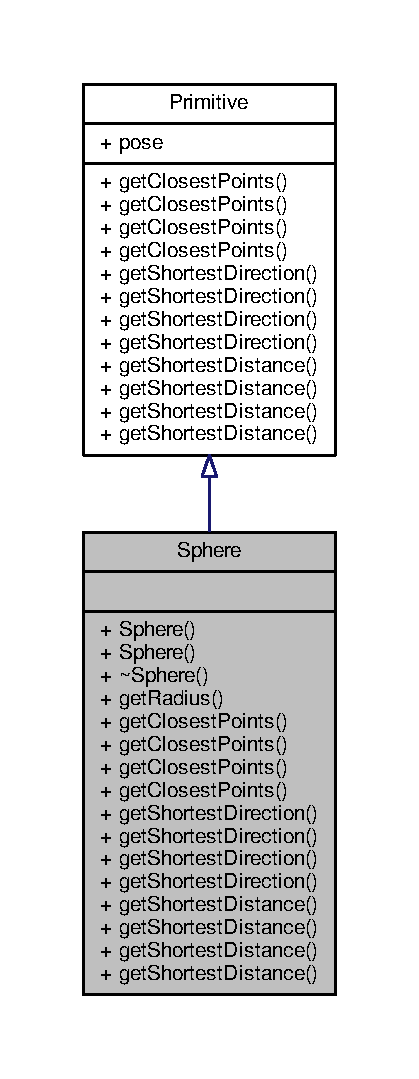
\includegraphics[width=201pt]{class_sphere__inherit__graph}
\end{center}
\end{figure}


Collaboration diagram for Sphere\+:
\nopagebreak
\begin{figure}[H]
\begin{center}
\leavevmode
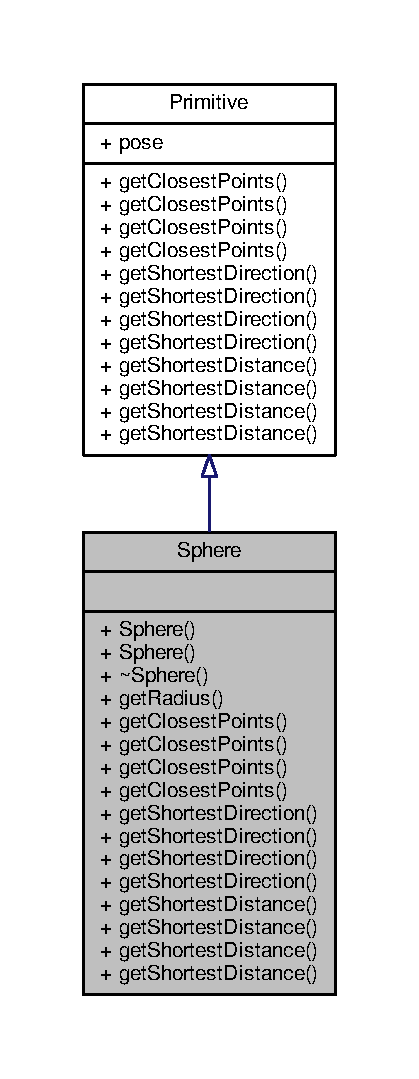
\includegraphics[width=201pt]{class_sphere__coll__graph}
\end{center}
\end{figure}
\subsection*{Public Member Functions}
\begin{DoxyCompactItemize}
\item 
\hyperlink{class_sphere_a7a9a9cfc01f619bb8cda60ae907d6372}{Sphere} (Eigen\+::\+Matrix4d \hyperlink{class_primitive_ad8b2afbad412f6046783d155c88fe312}{pose}, double radius)
\item 
\hyperlink{class_sphere_a564eb09ed988535e33c2b2e701d80581}{Sphere} (\hyperlink{class_sphere}{Sphere} $\ast$sphere)
\item 
\hyperlink{class_sphere_a569c071e50a3e11f678630ee1a17737e}{$\sim$\+Sphere} ()
\item 
float \hyperlink{class_sphere_a330dd34c7c7b6dfff106c4c71ec80028}{get\+Radius} ()
\item 
void \hyperlink{class_sphere_a9290773136dacf81a9f147343a7a0486}{get\+Closest\+Points} (Eigen\+::\+Matrix\+Xd \&closest\+Points, \hyperlink{class_primitive}{Primitive} $\ast$primitive)
\item 
void \hyperlink{class_sphere_a903c1c7a459e0c048b6f36a4f1376256}{get\+Closest\+Points} (Eigen\+::\+Matrix\+Xd \&closest\+Points, \hyperlink{class_capsule}{Capsule} $\ast$capsule)
\item 
void \hyperlink{class_sphere_ac2584cb5fb1d066a9527f8c95435093b}{get\+Closest\+Points} (Eigen\+::\+Matrix\+Xd \&closest\+Points, \hyperlink{class_sphere}{Sphere} $\ast$sphere)
\item 
void \hyperlink{class_sphere_a707fc14e03a6ff67ac012a18b2a8cb28}{get\+Shortest\+Direction} (Eigen\+::\+Vector3d \&shortest\+Direction, \hyperlink{class_primitive}{Primitive} $\ast$primitive)
\item 
void \hyperlink{class_sphere_af7ff30023363261cf118d1fb80c745a7}{get\+Shortest\+Direction} (Eigen\+::\+Vector3d \&shortest\+Direction, \hyperlink{class_capsule}{Capsule} $\ast$capsule)
\item 
void \hyperlink{class_sphere_a719592bc6a8307060f49f289da631310}{get\+Shortest\+Direction} (Eigen\+::\+Vector3d \&shortest\+Direction, \hyperlink{class_sphere}{Sphere} $\ast$sphere)
\item 
double \hyperlink{class_sphere_a7330816427e4099f4a8ccb8c34bd9ec6}{get\+Shortest\+Distance} (\hyperlink{class_primitive}{Primitive} $\ast$primitive)
\item 
double \hyperlink{class_sphere_a2b078585c4b272e9286eac12189b885b}{get\+Shortest\+Distance} (\hyperlink{class_capsule}{Capsule} $\ast$capsule)
\item 
double \hyperlink{class_sphere_a6efb9b513c9b42a7b040969b802727ea}{get\+Shortest\+Distance} (\hyperlink{class_sphere}{Sphere} $\ast$sphere)
\end{DoxyCompactItemize}
\subsection*{Additional Inherited Members}


\subsection{Detailed Description}
The \hyperlink{class_sphere}{Sphere} class

This class is a shape that inherits from primitive. 

Definition at line 290 of file primitives.\+h.



\subsection{Constructor \& Destructor Documentation}
\index{Sphere@{Sphere}!Sphere@{Sphere}}
\index{Sphere@{Sphere}!Sphere@{Sphere}}
\subsubsection[{\texorpdfstring{Sphere(\+Eigen\+::\+Matrix4d pose, double radius)}{Sphere(Eigen::Matrix4d pose, double radius)}}]{\setlength{\rightskip}{0pt plus 5cm}Sphere\+::\+Sphere (
\begin{DoxyParamCaption}
\item[{Eigen\+::\+Matrix4d}]{pose, }
\item[{double}]{radius}
\end{DoxyParamCaption}
)}\hypertarget{class_sphere_a7a9a9cfc01f619bb8cda60ae907d6372}{}\label{class_sphere_a7a9a9cfc01f619bb8cda60ae907d6372}
Constructor of \hyperlink{class_capsule}{Capsule} class


\begin{DoxyParams}{Parameters}
{\em pose} & center point of the line represented with a Matrix4d. \\
\hline
{\em radius} & radius of the sphere \\
\hline
\end{DoxyParams}


Definition at line 311 of file primitives.\+cpp.

\index{Sphere@{Sphere}!Sphere@{Sphere}}
\index{Sphere@{Sphere}!Sphere@{Sphere}}
\subsubsection[{\texorpdfstring{Sphere(\+Sphere $\ast$sphere)}{Sphere(Sphere *sphere)}}]{\setlength{\rightskip}{0pt plus 5cm}Sphere\+::\+Sphere (
\begin{DoxyParamCaption}
\item[{{\bf Sphere} $\ast$}]{sphere}
\end{DoxyParamCaption}
)}\hypertarget{class_sphere_a564eb09ed988535e33c2b2e701d80581}{}\label{class_sphere_a564eb09ed988535e33c2b2e701d80581}
Copy costructor of capsule class


\begin{DoxyParams}{Parameters}
{\em sphere} & The \hyperlink{class_sphere}{Sphere} instance to copy \\
\hline
\end{DoxyParams}


Definition at line 316 of file primitives.\+cpp.

\index{Sphere@{Sphere}!````~Sphere@{$\sim$\+Sphere}}
\index{````~Sphere@{$\sim$\+Sphere}!Sphere@{Sphere}}
\subsubsection[{\texorpdfstring{$\sim$\+Sphere()}{~Sphere()}}]{\setlength{\rightskip}{0pt plus 5cm}Sphere\+::$\sim$\+Sphere (
\begin{DoxyParamCaption}
{}
\end{DoxyParamCaption}
)}\hypertarget{class_sphere_a569c071e50a3e11f678630ee1a17737e}{}\label{class_sphere_a569c071e50a3e11f678630ee1a17737e}


Definition at line 321 of file primitives.\+cpp.



\subsection{Member Function Documentation}
\index{Sphere@{Sphere}!get\+Closest\+Points@{get\+Closest\+Points}}
\index{get\+Closest\+Points@{get\+Closest\+Points}!Sphere@{Sphere}}
\subsubsection[{\texorpdfstring{get\+Closest\+Points(\+Eigen\+::\+Matrix\+Xd \&closest\+Points, Primitive $\ast$primitive)}{getClosestPoints(Eigen::MatrixXd &closestPoints, Primitive *primitive)}}]{\setlength{\rightskip}{0pt plus 5cm}void Sphere\+::get\+Closest\+Points (
\begin{DoxyParamCaption}
\item[{Eigen\+::\+Matrix\+Xd \&}]{closest\+Points, }
\item[{{\bf Primitive} $\ast$}]{primitive}
\end{DoxyParamCaption}
)\hspace{0.3cm}{\ttfamily [virtual]}}\hypertarget{class_sphere_a9290773136dacf81a9f147343a7a0486}{}\label{class_sphere_a9290773136dacf81a9f147343a7a0486}
Performs a dynamic cast to overload the direction functions

This method takes an object that inherits from primitive and performs a dynamic cast to call the correct get\+Closest\+Points method depending on the class of the shape.


\begin{DoxyParams}[1]{Parameters}
 & {\em primitive} & address of the primitive object. \\
\hline
\mbox{\tt out}  & {\em closest\+Points} & the closest points in this primitive and primitive \\
\hline
\end{DoxyParams}


Implements \hyperlink{class_primitive_ae838e4e129f05642994da59f08f85f56}{Primitive}.



Definition at line 329 of file primitives.\+cpp.

\index{Sphere@{Sphere}!get\+Closest\+Points@{get\+Closest\+Points}}
\index{get\+Closest\+Points@{get\+Closest\+Points}!Sphere@{Sphere}}
\subsubsection[{\texorpdfstring{get\+Closest\+Points(\+Eigen\+::\+Matrix\+Xd \&closest\+Points, Capsule $\ast$capsule)}{getClosestPoints(Eigen::MatrixXd &closestPoints, Capsule *capsule)}}]{\setlength{\rightskip}{0pt plus 5cm}void Sphere\+::get\+Closest\+Points (
\begin{DoxyParamCaption}
\item[{Eigen\+::\+Matrix\+Xd \&}]{closest\+Points, }
\item[{{\bf Capsule} $\ast$}]{capsule}
\end{DoxyParamCaption}
)\hspace{0.3cm}{\ttfamily [virtual]}}\hypertarget{class_sphere_a903c1c7a459e0c048b6f36a4f1376256}{}\label{class_sphere_a903c1c7a459e0c048b6f36a4f1376256}
Finds the shortest distance between this primitive and a \hyperlink{class_capsule}{Capsule} primitive

This method takes a capsule object and returns the closest points in this primitive and in a capsule object.


\begin{DoxyParams}[1]{Parameters}
 & {\em capsule} & address of the primitive object \\
\hline
\mbox{\tt out}  & {\em closest\+Points} & the closest points in this primitive and capsule \\
\hline
\end{DoxyParams}


Implements \hyperlink{class_primitive_a2b8b8dea111d9eda31f72e06b47e9aa9}{Primitive}.



Definition at line 343 of file primitives.\+cpp.

\index{Sphere@{Sphere}!get\+Closest\+Points@{get\+Closest\+Points}}
\index{get\+Closest\+Points@{get\+Closest\+Points}!Sphere@{Sphere}}
\subsubsection[{\texorpdfstring{get\+Closest\+Points(\+Eigen\+::\+Matrix\+Xd \&closest\+Points, Sphere $\ast$sphere)}{getClosestPoints(Eigen::MatrixXd &closestPoints, Sphere *sphere)}}]{\setlength{\rightskip}{0pt plus 5cm}void Sphere\+::get\+Closest\+Points (
\begin{DoxyParamCaption}
\item[{Eigen\+::\+Matrix\+Xd \&}]{closest\+Points, }
\item[{{\bf Sphere} $\ast$}]{sphere}
\end{DoxyParamCaption}
)\hspace{0.3cm}{\ttfamily [virtual]}}\hypertarget{class_sphere_ac2584cb5fb1d066a9527f8c95435093b}{}\label{class_sphere_ac2584cb5fb1d066a9527f8c95435093b}
Finds the shortest distance between this primitive and a \hyperlink{class_sphere}{Sphere} primitive

This method takes a capsule object and returns the closest points in this primitive and in a sphere object.


\begin{DoxyParams}[1]{Parameters}
 & {\em sphere} & address of the primitive object \\
\hline
\mbox{\tt out}  & {\em closest\+Points} & the closest points in this primitive and sphere \\
\hline
\end{DoxyParams}


Implements \hyperlink{class_primitive_ac86ef47d59c21448ce78c91490c7dbd4}{Primitive}.



Definition at line 361 of file primitives.\+cpp.

\index{Sphere@{Sphere}!get\+Radius@{get\+Radius}}
\index{get\+Radius@{get\+Radius}!Sphere@{Sphere}}
\subsubsection[{\texorpdfstring{get\+Radius()}{getRadius()}}]{\setlength{\rightskip}{0pt plus 5cm}float Sphere\+::get\+Radius (
\begin{DoxyParamCaption}
{}
\end{DoxyParamCaption}
)}\hypertarget{class_sphere_a330dd34c7c7b6dfff106c4c71ec80028}{}\label{class_sphere_a330dd34c7c7b6dfff106c4c71ec80028}
Getter of radius

\begin{DoxyReturn}{Returns}
the radius of the sphere 
\end{DoxyReturn}


Definition at line 325 of file primitives.\+cpp.

\index{Sphere@{Sphere}!get\+Shortest\+Direction@{get\+Shortest\+Direction}}
\index{get\+Shortest\+Direction@{get\+Shortest\+Direction}!Sphere@{Sphere}}
\subsubsection[{\texorpdfstring{get\+Shortest\+Direction(\+Eigen\+::\+Vector3d \&shortest\+Direction, Primitive $\ast$primitive)}{getShortestDirection(Eigen::Vector3d &shortestDirection, Primitive *primitive)}}]{\setlength{\rightskip}{0pt plus 5cm}void Sphere\+::get\+Shortest\+Direction (
\begin{DoxyParamCaption}
\item[{Eigen\+::\+Vector3d \&}]{shortest\+Direction, }
\item[{{\bf Primitive} $\ast$}]{primitive}
\end{DoxyParamCaption}
)\hspace{0.3cm}{\ttfamily [virtual]}}\hypertarget{class_sphere_a707fc14e03a6ff67ac012a18b2a8cb28}{}\label{class_sphere_a707fc14e03a6ff67ac012a18b2a8cb28}
Performs a dynamic cast to overload the direction functions

This method takes an object that inherits from primitive and performs a dynamic cast to call the correct get\+Shortest\+Direction method depending on the class of the shape.


\begin{DoxyParams}[1]{Parameters}
 & {\em primitive} & address of the primitive object. \\
\hline
\mbox{\tt out}  & {\em shortest\+Direction} & a vector in 3D that represents the closes direction between this and the second primitive. \\
\hline
\end{DoxyParams}


Implements \hyperlink{class_primitive_ae37bbdf5271bf278b19888e0428579a8}{Primitive}.



Definition at line 372 of file primitives.\+cpp.

\index{Sphere@{Sphere}!get\+Shortest\+Direction@{get\+Shortest\+Direction}}
\index{get\+Shortest\+Direction@{get\+Shortest\+Direction}!Sphere@{Sphere}}
\subsubsection[{\texorpdfstring{get\+Shortest\+Direction(\+Eigen\+::\+Vector3d \&shortest\+Direction, Capsule $\ast$capsule)}{getShortestDirection(Eigen::Vector3d &shortestDirection, Capsule *capsule)}}]{\setlength{\rightskip}{0pt plus 5cm}void Sphere\+::get\+Shortest\+Direction (
\begin{DoxyParamCaption}
\item[{Eigen\+::\+Vector3d \&}]{shortest\+Direction, }
\item[{{\bf Capsule} $\ast$}]{capsule}
\end{DoxyParamCaption}
)\hspace{0.3cm}{\ttfamily [virtual]}}\hypertarget{class_sphere_af7ff30023363261cf118d1fb80c745a7}{}\label{class_sphere_af7ff30023363261cf118d1fb80c745a7}
Finds the shortest distance between this primitive and a \hyperlink{class_capsule}{Capsule} primitive

This method takes a capsule object and returns the closest direction between this primitive and a capsule object.


\begin{DoxyParams}[1]{Parameters}
 & {\em capsule} & address of the primitive object \\
\hline
\mbox{\tt out}  & {\em shortest\+Direction} & a vector in 3D that represents the closes direction between the primitive and capsule \\
\hline
\end{DoxyParams}


Implements \hyperlink{class_primitive_af9bd724a6618bd76e41e5682caa25023}{Primitive}.



Definition at line 386 of file primitives.\+cpp.

\index{Sphere@{Sphere}!get\+Shortest\+Direction@{get\+Shortest\+Direction}}
\index{get\+Shortest\+Direction@{get\+Shortest\+Direction}!Sphere@{Sphere}}
\subsubsection[{\texorpdfstring{get\+Shortest\+Direction(\+Eigen\+::\+Vector3d \&shortest\+Direction, Sphere $\ast$sphere)}{getShortestDirection(Eigen::Vector3d &shortestDirection, Sphere *sphere)}}]{\setlength{\rightskip}{0pt plus 5cm}void Sphere\+::get\+Shortest\+Direction (
\begin{DoxyParamCaption}
\item[{Eigen\+::\+Vector3d \&}]{shortest\+Direction, }
\item[{{\bf Sphere} $\ast$}]{sphere}
\end{DoxyParamCaption}
)\hspace{0.3cm}{\ttfamily [virtual]}}\hypertarget{class_sphere_a719592bc6a8307060f49f289da631310}{}\label{class_sphere_a719592bc6a8307060f49f289da631310}
Finds the shortest distance between this primitive and a \hyperlink{class_sphere}{Sphere} primitive

This method takes a capsule object and returns the closest direction between this primitive and a sphere object.


\begin{DoxyParams}[1]{Parameters}
 & {\em sphere} & address of the primitive object \\
\hline
\mbox{\tt out}  & {\em shortest\+Direction} & a vector in 3D that represents the closes direction between the primitive and sphere \\
\hline
\end{DoxyParams}


Implements \hyperlink{class_primitive_a3f1bc91de29fa904657c1ba4c40eee53}{Primitive}.



Definition at line 397 of file primitives.\+cpp.

\index{Sphere@{Sphere}!get\+Shortest\+Distance@{get\+Shortest\+Distance}}
\index{get\+Shortest\+Distance@{get\+Shortest\+Distance}!Sphere@{Sphere}}
\subsubsection[{\texorpdfstring{get\+Shortest\+Distance(\+Primitive $\ast$primitive)}{getShortestDistance(Primitive *primitive)}}]{\setlength{\rightskip}{0pt plus 5cm}double Sphere\+::get\+Shortest\+Distance (
\begin{DoxyParamCaption}
\item[{{\bf Primitive} $\ast$}]{primitive}
\end{DoxyParamCaption}
)\hspace{0.3cm}{\ttfamily [virtual]}}\hypertarget{class_sphere_a7330816427e4099f4a8ccb8c34bd9ec6}{}\label{class_sphere_a7330816427e4099f4a8ccb8c34bd9ec6}
Performs a dynamic cast to overload the distance functions

This method takes an object that inherits from primitive and performs a dynamic cast to call the correct get\+Shortest\+Distance method depending on the class of the shape. returns a double value.


\begin{DoxyParams}{Parameters}
{\em primitive} & address of the primitive object. \\
\hline
\end{DoxyParams}
\begin{DoxyReturn}{Returns}
the closest distance between this and the second primitive. 
\end{DoxyReturn}


Implements \hyperlink{class_primitive_a340b3e5540b910480ada939383985d66}{Primitive}.



Definition at line 408 of file primitives.\+cpp.

\index{Sphere@{Sphere}!get\+Shortest\+Distance@{get\+Shortest\+Distance}}
\index{get\+Shortest\+Distance@{get\+Shortest\+Distance}!Sphere@{Sphere}}
\subsubsection[{\texorpdfstring{get\+Shortest\+Distance(\+Capsule $\ast$capsule)}{getShortestDistance(Capsule *capsule)}}]{\setlength{\rightskip}{0pt plus 5cm}double Sphere\+::get\+Shortest\+Distance (
\begin{DoxyParamCaption}
\item[{{\bf Capsule} $\ast$}]{capsule}
\end{DoxyParamCaption}
)\hspace{0.3cm}{\ttfamily [virtual]}}\hypertarget{class_sphere_a2b078585c4b272e9286eac12189b885b}{}\label{class_sphere_a2b078585c4b272e9286eac12189b885b}
Finds the shortest distance between this primitive and a \hyperlink{class_capsule}{Capsule} primitive

This method takes a capsule object and returns the closest distance between this primitive and a capsule object. returns a double value.


\begin{DoxyParams}{Parameters}
{\em capsule} & address of the primitive object \\
\hline
\end{DoxyParams}
\begin{DoxyReturn}{Returns}
the closest distance between the primitive and capsule 
\end{DoxyReturn}


Implements \hyperlink{class_primitive_a46e60acfe4c005c0ec94e1e8b82d36db}{Primitive}.



Definition at line 422 of file primitives.\+cpp.

\index{Sphere@{Sphere}!get\+Shortest\+Distance@{get\+Shortest\+Distance}}
\index{get\+Shortest\+Distance@{get\+Shortest\+Distance}!Sphere@{Sphere}}
\subsubsection[{\texorpdfstring{get\+Shortest\+Distance(\+Sphere $\ast$sphere)}{getShortestDistance(Sphere *sphere)}}]{\setlength{\rightskip}{0pt plus 5cm}double Sphere\+::get\+Shortest\+Distance (
\begin{DoxyParamCaption}
\item[{{\bf Sphere} $\ast$}]{sphere}
\end{DoxyParamCaption}
)\hspace{0.3cm}{\ttfamily [virtual]}}\hypertarget{class_sphere_a6efb9b513c9b42a7b040969b802727ea}{}\label{class_sphere_a6efb9b513c9b42a7b040969b802727ea}
Finds the shortest distance between this primitive and a \hyperlink{class_sphere}{Sphere} primitive

This method takes a capsule object and returns the closest distance between this primitive and a sphere object. returns a double value.


\begin{DoxyParams}{Parameters}
{\em sphere} & address of the primitive object \\
\hline
\end{DoxyParams}
\begin{DoxyReturn}{Returns}
the closest distance between the primitive and sphere 
\end{DoxyReturn}


Implements \hyperlink{class_primitive_adaac4fc4fedf9cd76d4eb9c77e9ae560}{Primitive}.



Definition at line 432 of file primitives.\+cpp.



The documentation for this class was generated from the following files\+:\begin{DoxyCompactItemize}
\item 
\hyperlink{primitives_8h}{primitives.\+h}\item 
\hyperlink{primitives_8cpp}{primitives.\+cpp}\end{DoxyCompactItemize}

\chapter{File Documentation}
\hypertarget{arm_8cpp}{}\section{arm.\+cpp File Reference}
\label{arm_8cpp}\index{arm.\+cpp@{arm.\+cpp}}
{\ttfamily \#include \char`\"{}arm.\+h\char`\"{}}\\*
Include dependency graph for arm.\+cpp\+:
\nopagebreak
\begin{figure}[H]
\begin{center}
\leavevmode
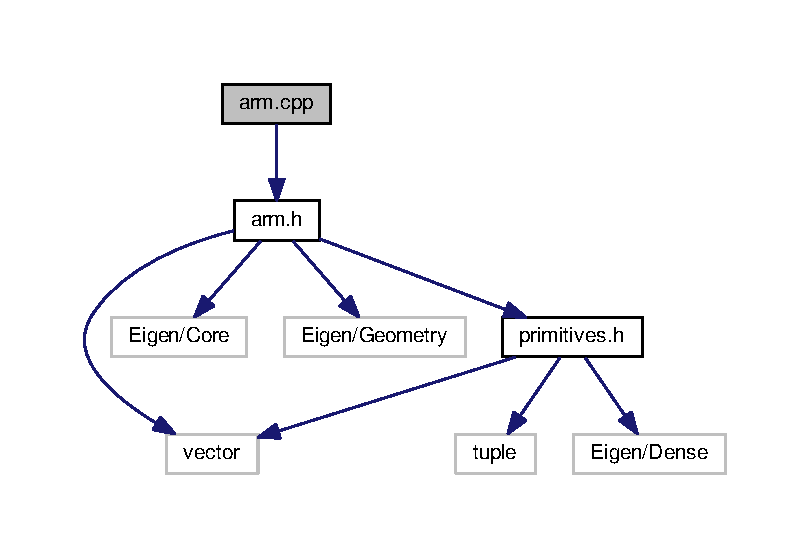
\includegraphics[width=350pt]{arm_8cpp__incl}
\end{center}
\end{figure}

\hypertarget{arm_8h}{}\section{arm.\+h File Reference}
\label{arm_8h}\index{arm.\+h@{arm.\+h}}
{\ttfamily \#include $<$vector$>$}\\*
{\ttfamily \#include $<$Eigen/\+Core$>$}\\*
{\ttfamily \#include $<$Eigen/\+Geometry$>$}\\*
{\ttfamily \#include \char`\"{}primitives.\+h\char`\"{}}\\*
Include dependency graph for arm.\+h\+:
\nopagebreak
\begin{figure}[H]
\begin{center}
\leavevmode
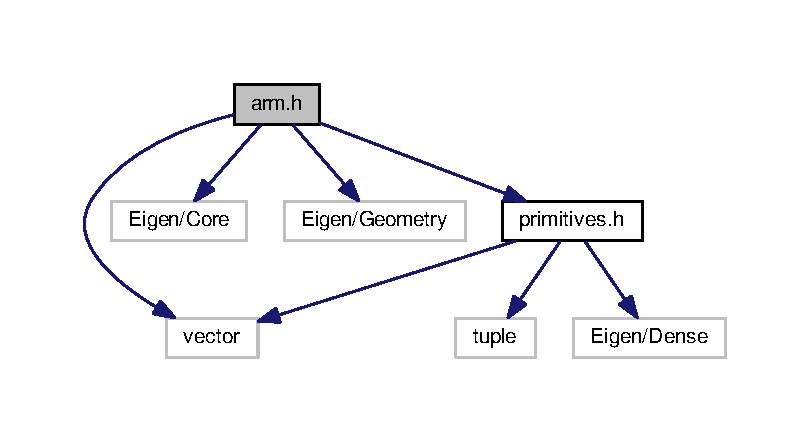
\includegraphics[width=350pt]{arm_8h__incl}
\end{center}
\end{figure}
This graph shows which files directly or indirectly include this file\+:
\nopagebreak
\begin{figure}[H]
\begin{center}
\leavevmode
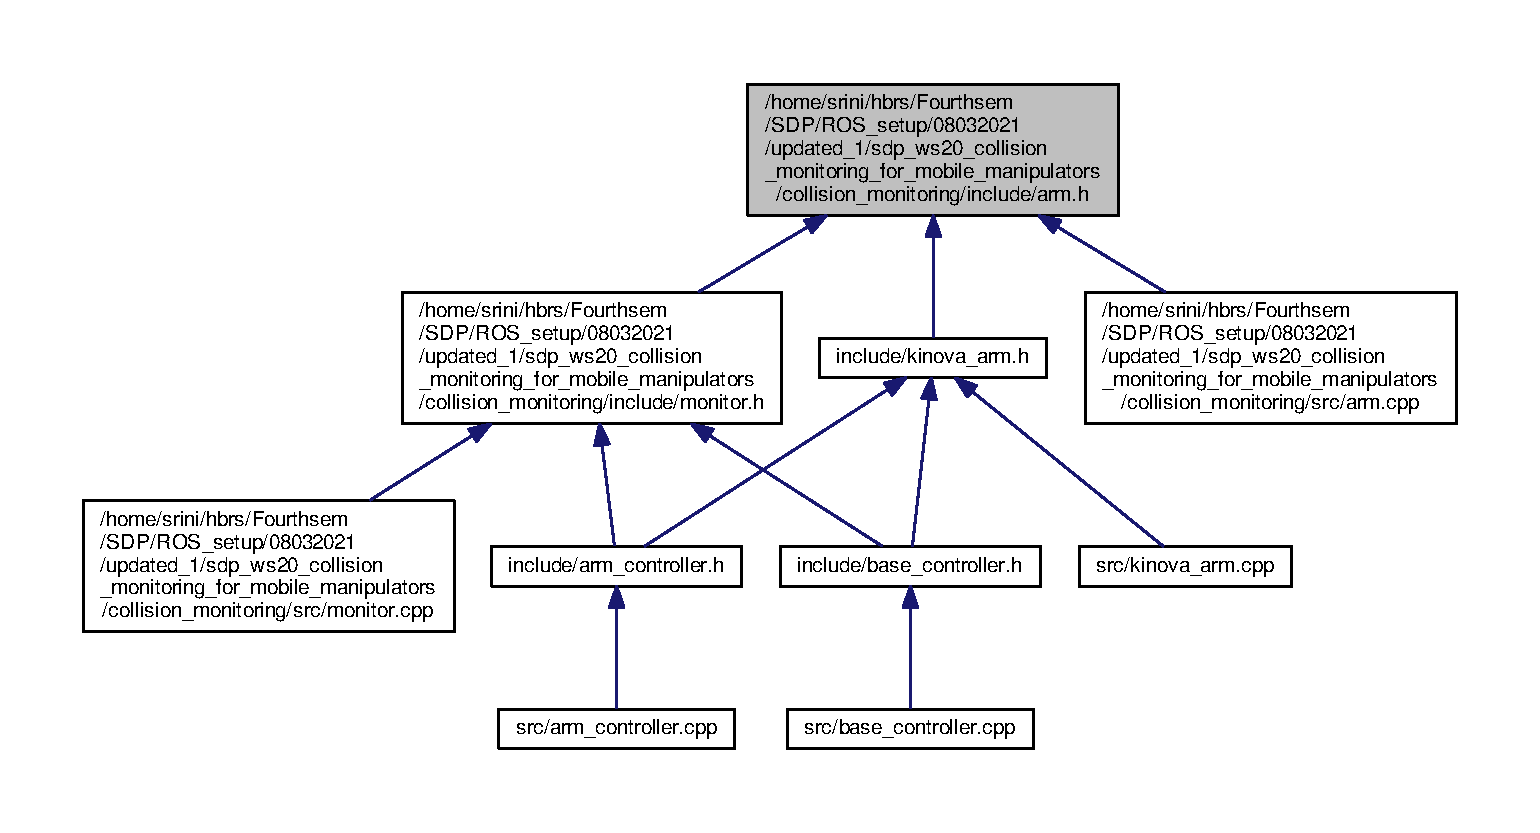
\includegraphics[width=350pt]{arm_8h__dep__incl}
\end{center}
\end{figure}
\subsection*{Classes}
\begin{DoxyCompactItemize}
\item 
class \hyperlink{class_arm}{Arm}
\end{DoxyCompactItemize}

\hypertarget{arm__controller_8cpp}{}\section{src/arm\+\_\+controller.cpp File Reference}
\label{arm__controller_8cpp}\index{src/arm\+\_\+controller.\+cpp@{src/arm\+\_\+controller.\+cpp}}
{\ttfamily \#include \char`\"{}arm\+\_\+controller.\+h\char`\"{}}\\*
{\ttfamily \#include $<$ros/console.\+h$>$}\\*
{\ttfamily \#include $<$ros/ros.\+h$>$}\\*
{\ttfamily \#include $<$std\+\_\+msgs/\+String.\+h$>$}\\*
Include dependency graph for arm\+\_\+controller.\+cpp\+:
\nopagebreak
\begin{figure}[H]
\begin{center}
\leavevmode
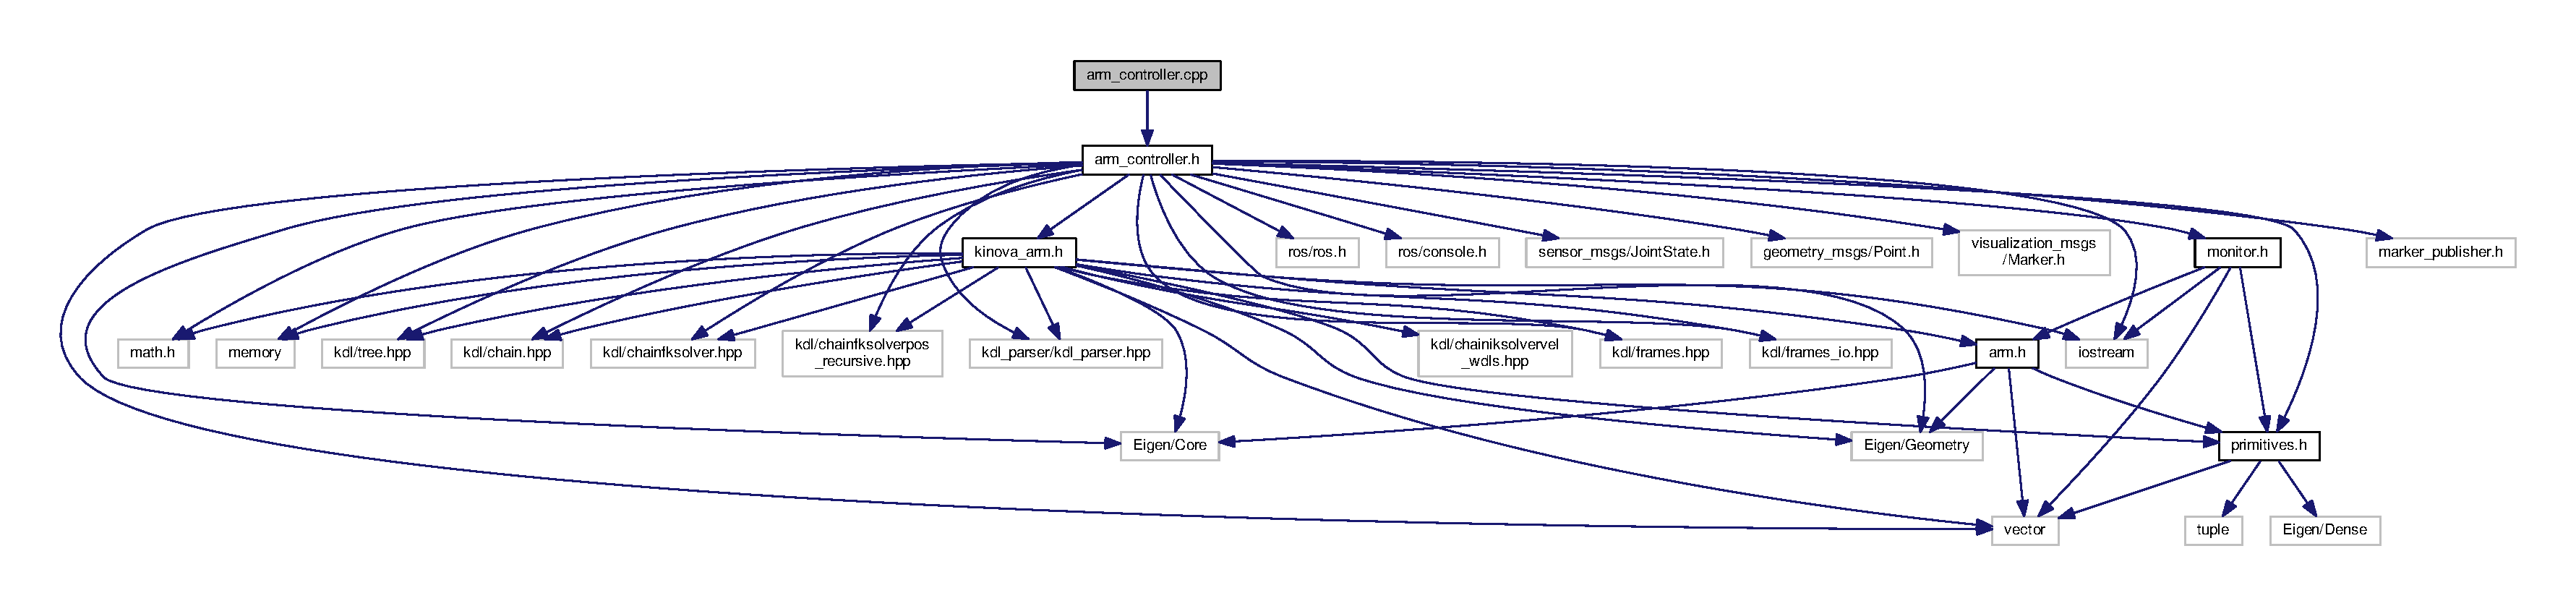
\includegraphics[width=350pt]{arm__controller_8cpp__incl}
\end{center}
\end{figure}
\subsection*{Macros}
\begin{DoxyCompactItemize}
\item 
\#define \hyperlink{arm__controller_8cpp_a598a3330b3c21701223ee0ca14316eca}{PI}~3.\+14159265
\end{DoxyCompactItemize}


\subsection{Macro Definition Documentation}
\index{arm\+\_\+controller.\+cpp@{arm\+\_\+controller.\+cpp}!PI@{PI}}
\index{PI@{PI}!arm\+\_\+controller.\+cpp@{arm\+\_\+controller.\+cpp}}
\subsubsection[{\texorpdfstring{PI}{PI}}]{\setlength{\rightskip}{0pt plus 5cm}\#define PI~3.\+14159265}\hypertarget{arm__controller_8cpp_a598a3330b3c21701223ee0ca14316eca}{}\label{arm__controller_8cpp_a598a3330b3c21701223ee0ca14316eca}

\hypertarget{arm__controller_8h}{}\section{include/arm\+\_\+controller.h File Reference}
\label{arm__controller_8h}\index{include/arm\+\_\+controller.\+h@{include/arm\+\_\+controller.\+h}}
{\ttfamily \#include $<$vector$>$}\\*
{\ttfamily \#include $<$math.\+h$>$}\\*
{\ttfamily \#include $<$memory$>$}\\*
{\ttfamily \#include $<$iostream$>$}\\*
{\ttfamily \#include $<$Eigen/\+Core$>$}\\*
{\ttfamily \#include $<$Eigen/\+Geometry$>$}\\*
{\ttfamily \#include $<$kdl/tree.\+hpp$>$}\\*
{\ttfamily \#include $<$kdl/chain.\+hpp$>$}\\*
{\ttfamily \#include $<$kdl/chainfksolver.\+hpp$>$}\\*
{\ttfamily \#include $<$kdl/chainfksolverpos\+\_\+recursive.\+hpp$>$}\\*
{\ttfamily \#include $<$kdl\+\_\+parser/kdl\+\_\+parser.\+hpp$>$}\\*
{\ttfamily \#include $<$kdl/frames.\+hpp$>$}\\*
{\ttfamily \#include $<$kdl/frames\+\_\+io.\+hpp$>$}\\*
{\ttfamily \#include $<$ros/ros.\+h$>$}\\*
{\ttfamily \#include $<$ros/console.\+h$>$}\\*
{\ttfamily \#include $<$sensor\+\_\+msgs/\+Joint\+State.\+h$>$}\\*
{\ttfamily \#include $<$geometry\+\_\+msgs/\+Point.\+h$>$}\\*
{\ttfamily \#include $<$visualization\+\_\+msgs/\+Marker.\+h$>$}\\*
{\ttfamily \#include \char`\"{}primitives.\+h\char`\"{}}\\*
{\ttfamily \#include \char`\"{}kinova\+\_\+arm.\+h\char`\"{}}\\*
{\ttfamily \#include \char`\"{}monitor.\+h\char`\"{}}\\*
{\ttfamily \#include \char`\"{}marker\+\_\+publisher.\+h\char`\"{}}\\*
Include dependency graph for arm\+\_\+controller.\+h\+:
\nopagebreak
\begin{figure}[H]
\begin{center}
\leavevmode
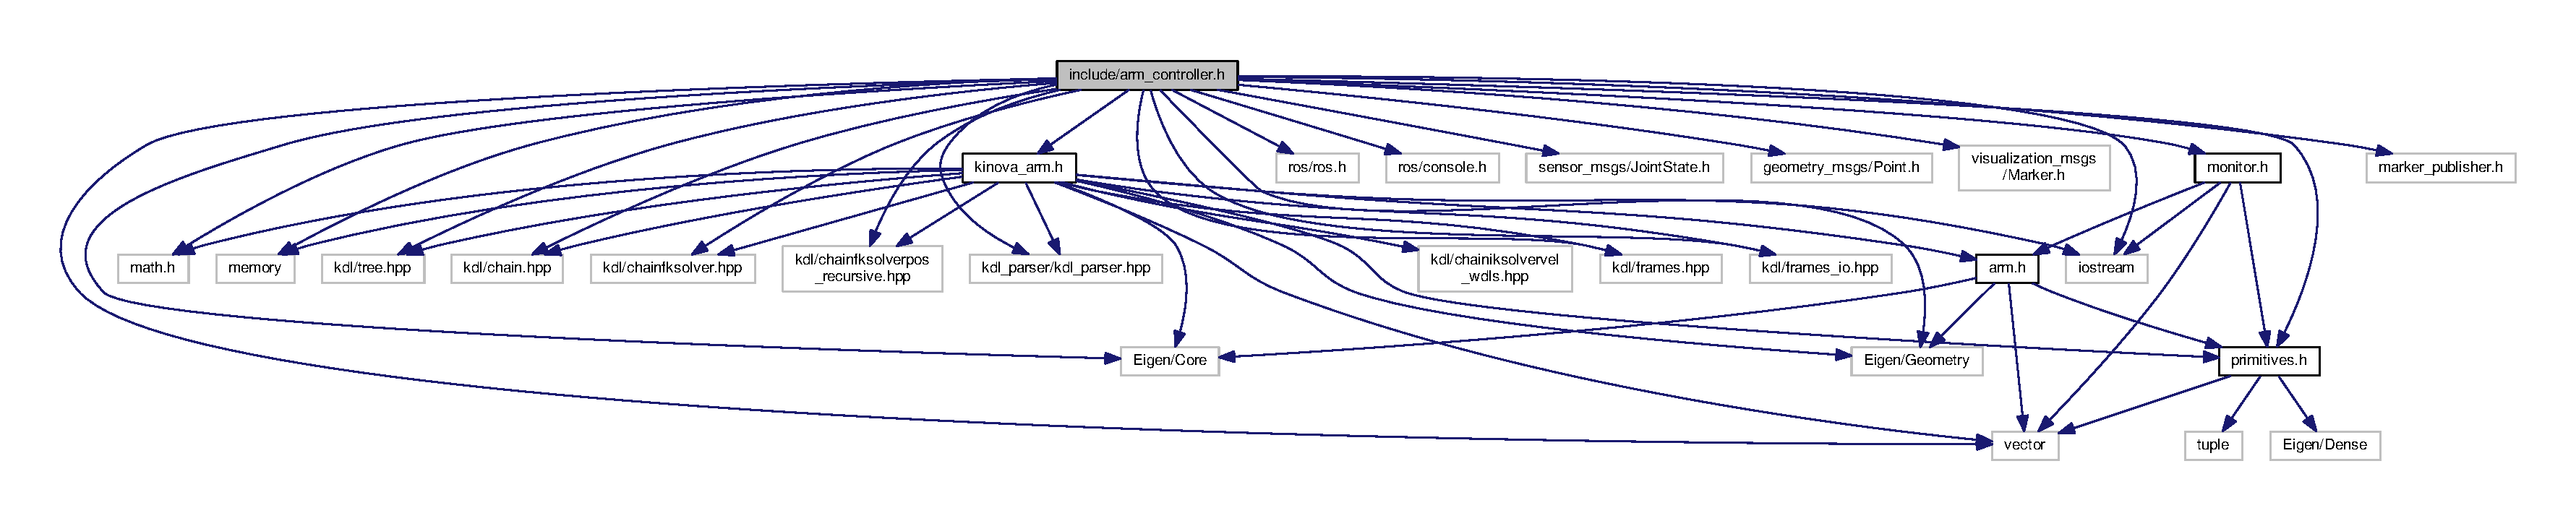
\includegraphics[width=350pt]{arm__controller_8h__incl}
\end{center}
\end{figure}
This graph shows which files directly or indirectly include this file\+:
\nopagebreak
\begin{figure}[H]
\begin{center}
\leavevmode
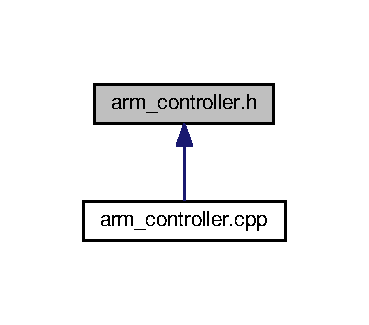
\includegraphics[width=200pt]{arm__controller_8h__dep__incl}
\end{center}
\end{figure}
\subsection*{Classes}
\begin{DoxyCompactItemize}
\item 
class \hyperlink{class_rviz_obstacle}{Rviz\+Obstacle}
\item 
class \hyperlink{class_arm_controller}{Arm\+Controller}
\end{DoxyCompactItemize}

\hypertarget{kinova__arm_8cpp}{}\section{kinova\+\_\+arm.\+cpp File Reference}
\label{kinova__arm_8cpp}\index{kinova\+\_\+arm.\+cpp@{kinova\+\_\+arm.\+cpp}}
{\ttfamily \#include \char`\"{}kinova\+\_\+arm.\+h\char`\"{}}\\*
Include dependency graph for kinova\+\_\+arm.\+cpp\+:\nopagebreak
\begin{figure}[H]
\begin{center}
\leavevmode
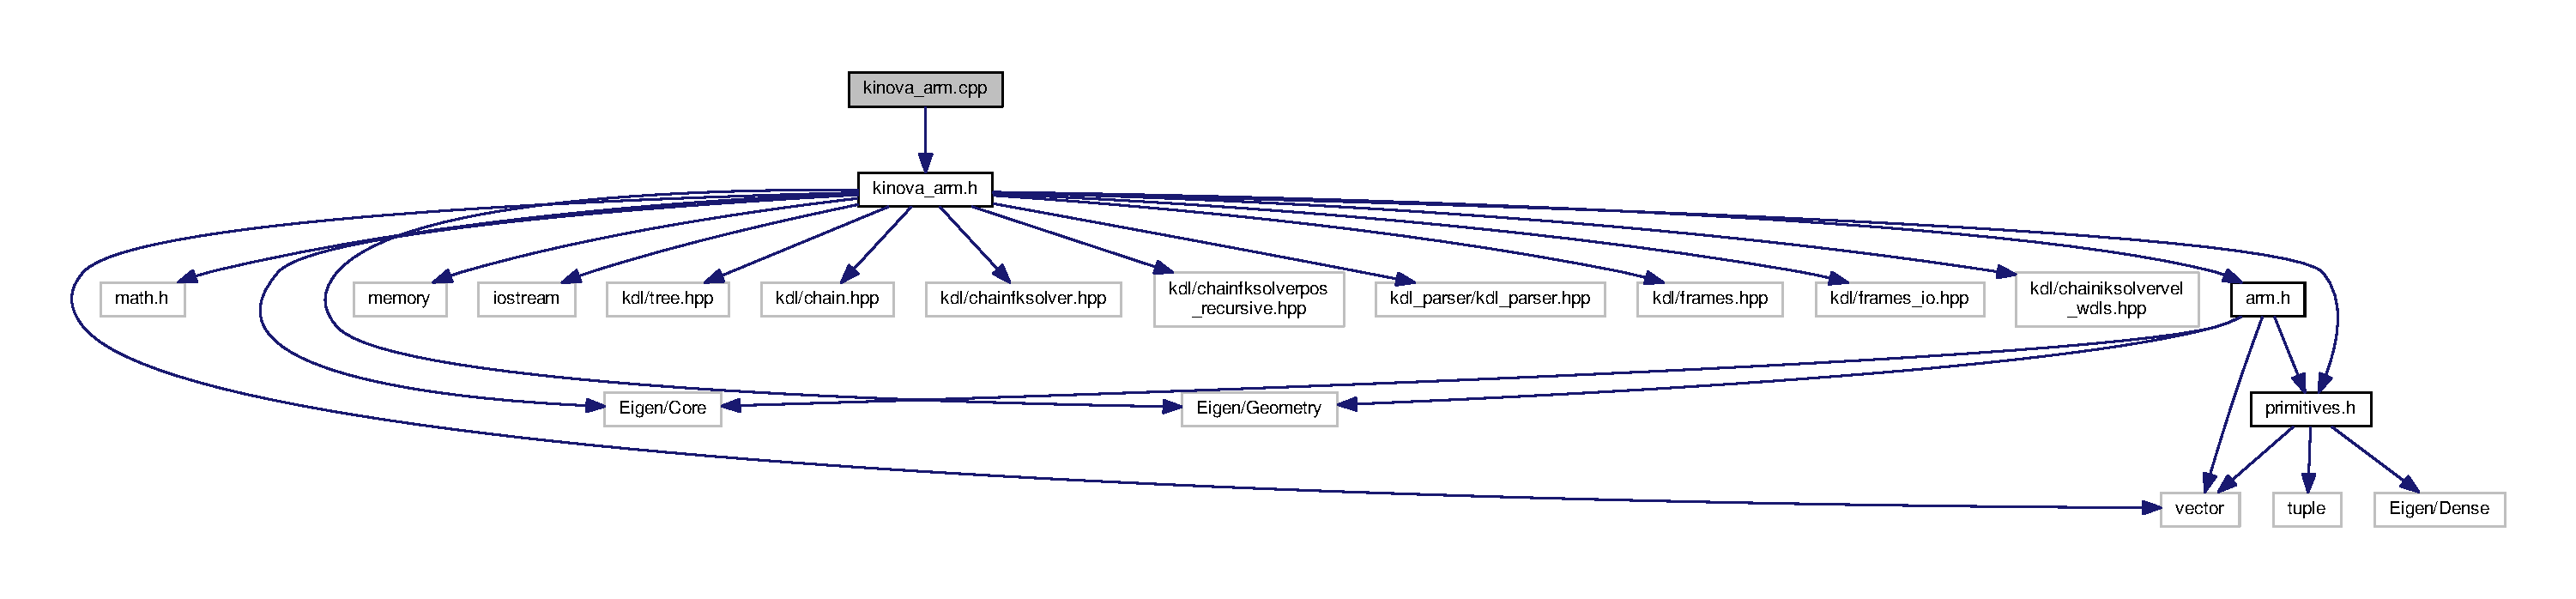
\includegraphics[width=350pt]{kinova__arm_8cpp__incl}
\end{center}
\end{figure}
\subsection*{Macros}
\begin{DoxyCompactItemize}
\item 
\#define \hyperlink{kinova__arm_8cpp_a7fefc67ecba9779f456f15e8236d780a}{M\+A\+X\+\_\+\+J\+O\+I\+N\+T\+\_\+\+V\+EL}~10
\end{DoxyCompactItemize}


\subsection{Macro Definition Documentation}
\index{kinova\+\_\+arm.\+cpp@{kinova\+\_\+arm.\+cpp}!M\+A\+X\+\_\+\+J\+O\+I\+N\+T\+\_\+\+V\+EL@{M\+A\+X\+\_\+\+J\+O\+I\+N\+T\+\_\+\+V\+EL}}
\index{M\+A\+X\+\_\+\+J\+O\+I\+N\+T\+\_\+\+V\+EL@{M\+A\+X\+\_\+\+J\+O\+I\+N\+T\+\_\+\+V\+EL}!kinova\+\_\+arm.\+cpp@{kinova\+\_\+arm.\+cpp}}
\subsubsection[{\texorpdfstring{M\+A\+X\+\_\+\+J\+O\+I\+N\+T\+\_\+\+V\+EL}{MAX_JOINT_VEL}}]{\setlength{\rightskip}{0pt plus 5cm}\#define M\+A\+X\+\_\+\+J\+O\+I\+N\+T\+\_\+\+V\+EL~10}\hypertarget{kinova__arm_8cpp_a7fefc67ecba9779f456f15e8236d780a}{}\label{kinova__arm_8cpp_a7fefc67ecba9779f456f15e8236d780a}


Definition at line 2 of file kinova\+\_\+arm.\+cpp.


\hypertarget{kinova__arm_8h}{}\section{include/kinova\+\_\+arm.h File Reference}
\label{kinova__arm_8h}\index{include/kinova\+\_\+arm.\+h@{include/kinova\+\_\+arm.\+h}}
{\ttfamily \#include $<$vector$>$}\\*
{\ttfamily \#include $<$math.\+h$>$}\\*
{\ttfamily \#include $<$Eigen/\+Core$>$}\\*
{\ttfamily \#include $<$Eigen/\+Geometry$>$}\\*
{\ttfamily \#include $<$memory$>$}\\*
{\ttfamily \#include $<$iostream$>$}\\*
{\ttfamily \#include $<$kdl/tree.\+hpp$>$}\\*
{\ttfamily \#include $<$kdl/chain.\+hpp$>$}\\*
{\ttfamily \#include $<$kdl/chainfksolver.\+hpp$>$}\\*
{\ttfamily \#include $<$kdl/chainfksolverpos\+\_\+recursive.\+hpp$>$}\\*
{\ttfamily \#include $<$kdl\+\_\+parser/kdl\+\_\+parser.\+hpp$>$}\\*
{\ttfamily \#include $<$kdl/frames.\+hpp$>$}\\*
{\ttfamily \#include $<$kdl/frames\+\_\+io.\+hpp$>$}\\*
{\ttfamily \#include $<$kdl/chainiksolvervel\+\_\+wdls.\+hpp$>$}\\*
{\ttfamily \#include \char`\"{}primitives.\+h\char`\"{}}\\*
{\ttfamily \#include \char`\"{}arm.\+h\char`\"{}}\\*
Include dependency graph for kinova\+\_\+arm.\+h\+:
\nopagebreak
\begin{figure}[H]
\begin{center}
\leavevmode
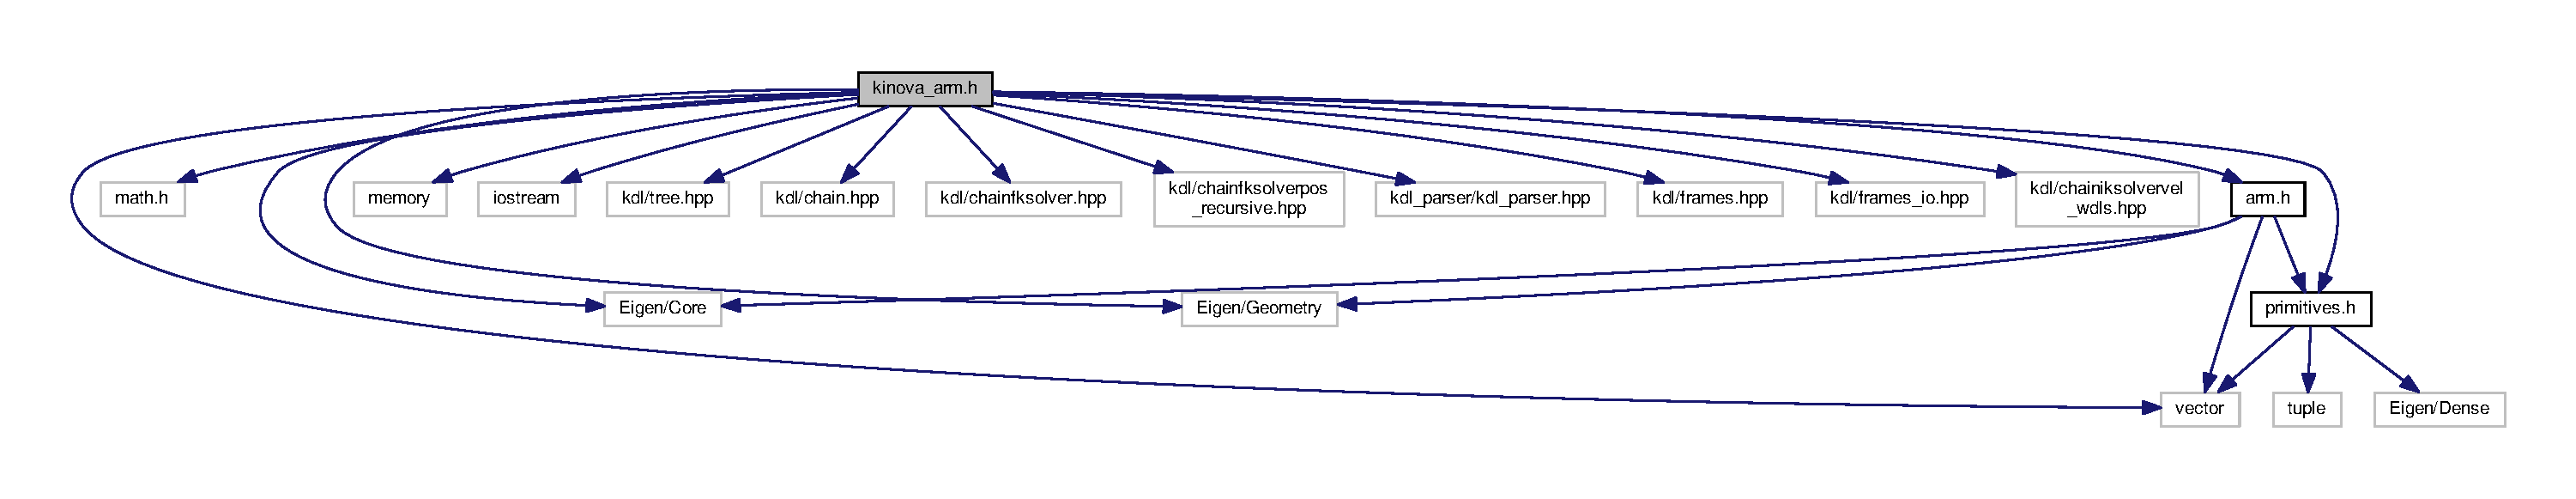
\includegraphics[width=350pt]{kinova__arm_8h__incl}
\end{center}
\end{figure}
This graph shows which files directly or indirectly include this file\+:
\nopagebreak
\begin{figure}[H]
\begin{center}
\leavevmode
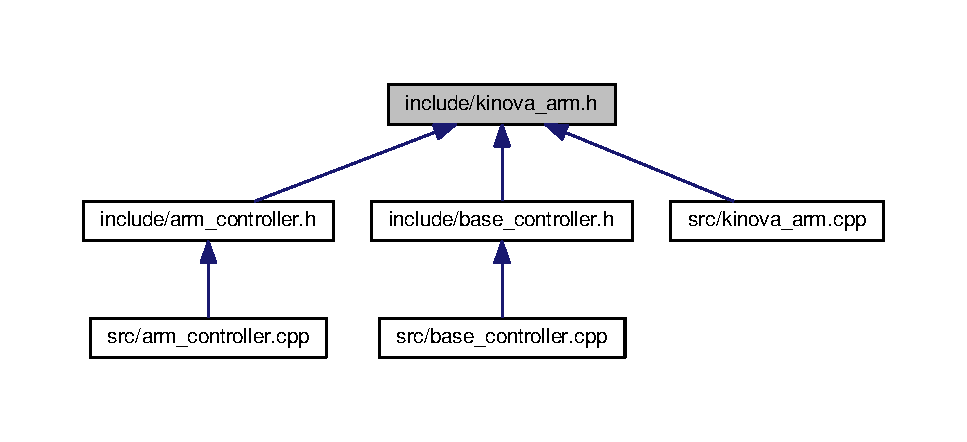
\includegraphics[width=350pt]{kinova__arm_8h__dep__incl}
\end{center}
\end{figure}
\subsection*{Classes}
\begin{DoxyCompactItemize}
\item 
class \hyperlink{class_kinova_arm}{Kinova\+Arm}
\item 
class \hyperlink{class_narkin_base}{Narkin\+Base}
\end{DoxyCompactItemize}

\hypertarget{_l_i_c_e_n_s_e_8md}{}\section{L\+I\+C\+E\+N\+S\+E.\+md File Reference}
\label{_l_i_c_e_n_s_e_8md}\index{L\+I\+C\+E\+N\+S\+E.\+md@{L\+I\+C\+E\+N\+S\+E.\+md}}

\hypertarget{monitor_8cpp}{}\section{monitor.\+cpp File Reference}
\label{monitor_8cpp}\index{monitor.\+cpp@{monitor.\+cpp}}
{\ttfamily \#include \char`\"{}monitor.\+h\char`\"{}}\\*
{\ttfamily \#include $<$vector$>$}\\*
{\ttfamily \#include $<$typeinfo$>$}\\*
Include dependency graph for monitor.\+cpp\+:\nopagebreak
\begin{figure}[H]
\begin{center}
\leavevmode
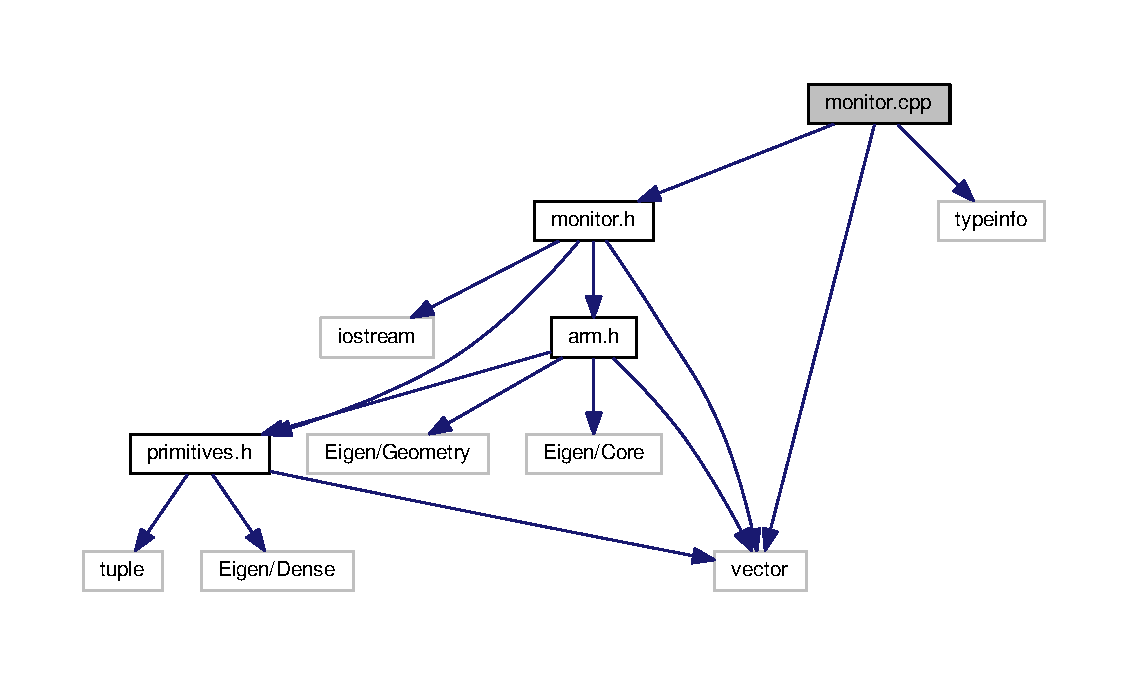
\includegraphics[width=350pt]{monitor_8cpp__incl}
\end{center}
\end{figure}

\hypertarget{monitor_8h}{}\section{/home/srini/hbrs/\+Fourthsem/\+S\+D\+P/\+R\+O\+S\+\_\+setup/08032021/updated\+\_\+1/sdp\+\_\+ws20\+\_\+collision\+\_\+monitoring\+\_\+for\+\_\+mobile\+\_\+manipulators/collision\+\_\+monitoring/include/monitor.h File Reference}
\label{monitor_8h}\index{/home/srini/hbrs/\+Fourthsem/\+S\+D\+P/\+R\+O\+S\+\_\+setup/08032021/updated\+\_\+1/sdp\+\_\+ws20\+\_\+collision\+\_\+monitoring\+\_\+for\+\_\+mobile\+\_\+manipulators/collision\+\_\+monitoring/include/monitor.\+h@{/home/srini/hbrs/\+Fourthsem/\+S\+D\+P/\+R\+O\+S\+\_\+setup/08032021/updated\+\_\+1/sdp\+\_\+ws20\+\_\+collision\+\_\+monitoring\+\_\+for\+\_\+mobile\+\_\+manipulators/collision\+\_\+monitoring/include/monitor.\+h}}
{\ttfamily \#include $<$vector$>$}\\*
{\ttfamily \#include $<$iostream$>$}\\*
{\ttfamily \#include \char`\"{}arm.\+h\char`\"{}}\\*
{\ttfamily \#include \char`\"{}primitives.\+h\char`\"{}}\\*
Include dependency graph for monitor.\+h\+:
\nopagebreak
\begin{figure}[H]
\begin{center}
\leavevmode
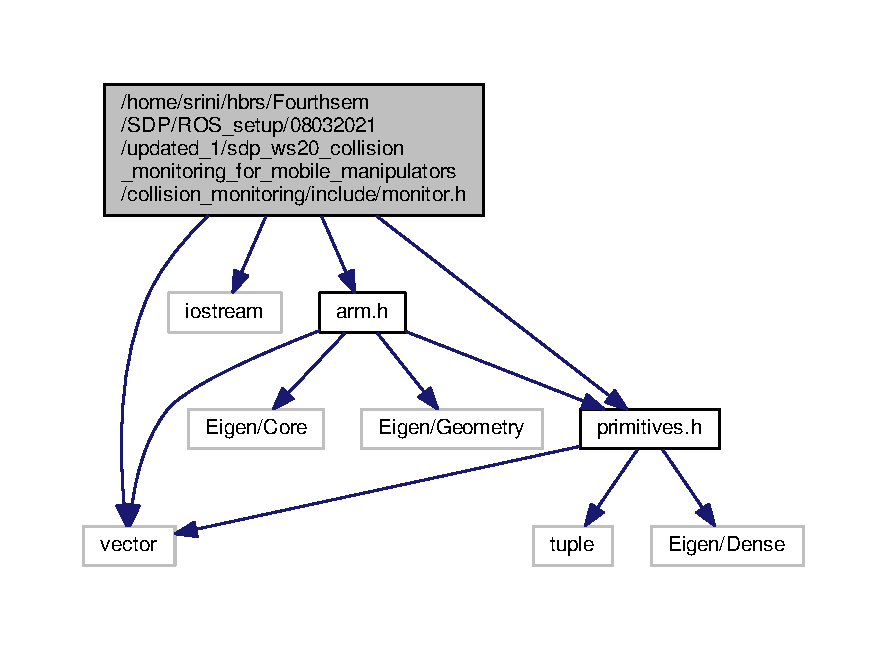
\includegraphics[width=350pt]{monitor_8h__incl}
\end{center}
\end{figure}
This graph shows which files directly or indirectly include this file\+:
\nopagebreak
\begin{figure}[H]
\begin{center}
\leavevmode
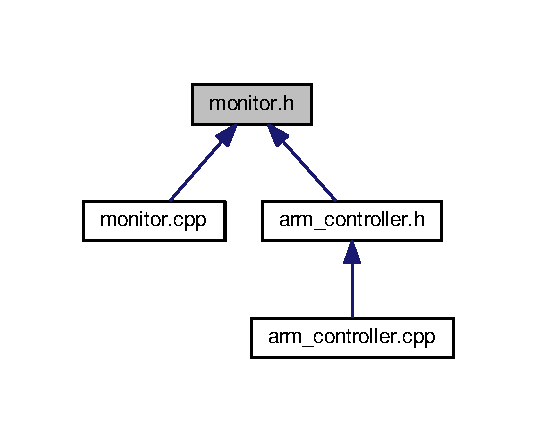
\includegraphics[width=350pt]{monitor_8h__dep__incl}
\end{center}
\end{figure}
\subsection*{Classes}
\begin{DoxyCompactItemize}
\item 
class \hyperlink{class_monitor}{Monitor}
\end{DoxyCompactItemize}

\hypertarget{primitives_8cpp}{}\section{primitives.\+cpp File Reference}
\label{primitives_8cpp}\index{primitives.\+cpp@{primitives.\+cpp}}
{\ttfamily \#include \char`\"{}primitives.\+h\char`\"{}}\\*
{\ttfamily \#include $<$math.\+h$>$}\\*
{\ttfamily \#include $<$iostream$>$}\\*
Include dependency graph for primitives.\+cpp\+:\nopagebreak
\begin{figure}[H]
\begin{center}
\leavevmode
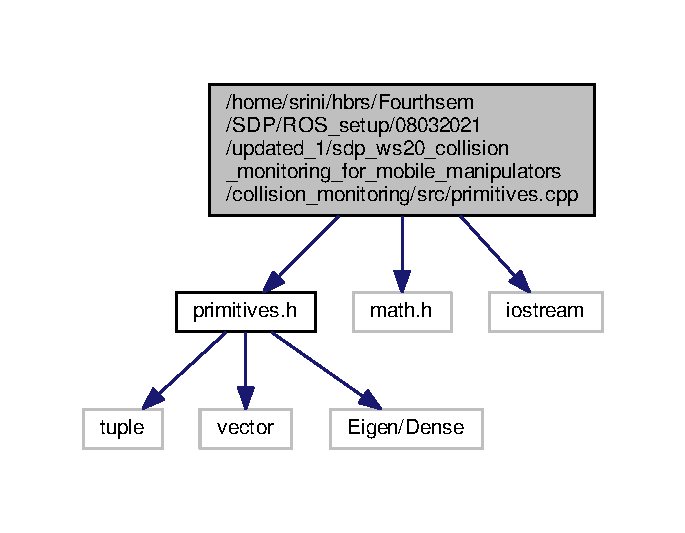
\includegraphics[width=329pt]{primitives_8cpp__incl}
\end{center}
\end{figure}

\hypertarget{primitives_8h}{}\section{primitives.\+h File Reference}
\label{primitives_8h}\index{primitives.\+h@{primitives.\+h}}
{\ttfamily \#include $<$tuple$>$}\\*
{\ttfamily \#include $<$vector$>$}\\*
{\ttfamily \#include $<$Eigen/\+Dense$>$}\\*
Include dependency graph for primitives.\+h\+:\nopagebreak
\begin{figure}[H]
\begin{center}
\leavevmode
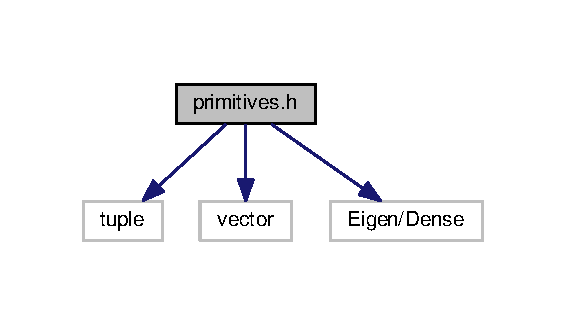
\includegraphics[width=272pt]{primitives_8h__incl}
\end{center}
\end{figure}
This graph shows which files directly or indirectly include this file\+:\nopagebreak
\begin{figure}[H]
\begin{center}
\leavevmode
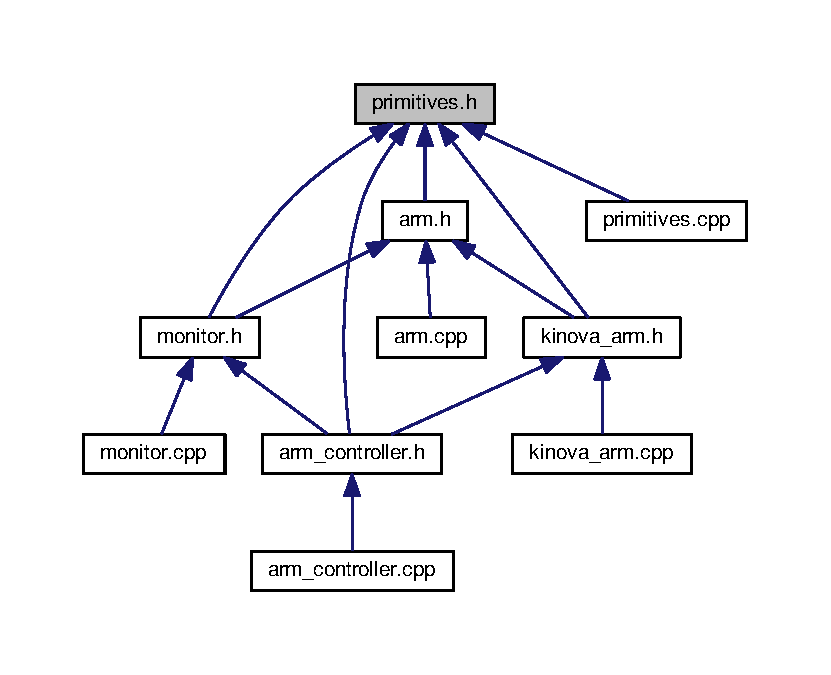
\includegraphics[width=350pt]{primitives_8h__dep__incl}
\end{center}
\end{figure}
\subsection*{Classes}
\begin{DoxyCompactItemize}
\item 
class \hyperlink{class_primitive}{Primitive}
\item 
class \hyperlink{class_line}{Line}
\item 
class \hyperlink{class_capsule}{Capsule}
\item 
class \hyperlink{class_sphere}{Sphere}
\end{DoxyCompactItemize}

\hypertarget{deliverables_2doxygen_2catkin__workspace_2_r_e_a_d_m_e_8md}{}\section{R\+E\+A\+D\+M\+E.\+md File Reference}
\label{deliverables_2doxygen_2catkin__workspace_2_r_e_a_d_m_e_8md}\index{R\+E\+A\+D\+M\+E.\+md@{R\+E\+A\+D\+M\+E.\+md}}

\hypertarget{collision__monitoring_2_r_e_a_d_m_e_8md}{}\section{R\+E\+A\+D\+M\+E.\+md File Reference}
\label{collision__monitoring_2_r_e_a_d_m_e_8md}\index{R\+E\+A\+D\+M\+E.\+md@{R\+E\+A\+D\+M\+E.\+md}}

\hypertarget{deliverables_2doxygen_2_r_e_a_d_m_e_8md}{}\section{R\+E\+A\+D\+M\+E.\+md File Reference}
\label{deliverables_2doxygen_2_r_e_a_d_m_e_8md}\index{R\+E\+A\+D\+M\+E.\+md@{R\+E\+A\+D\+M\+E.\+md}}

\hypertarget{deliverables_2doxygen_2src_2_r_e_a_d_m_e_8md}{}\section{R\+E\+A\+D\+M\+E.\+md File Reference}
\label{deliverables_2doxygen_2src_2_r_e_a_d_m_e_8md}\index{R\+E\+A\+D\+M\+E.\+md@{R\+E\+A\+D\+M\+E.\+md}}

%--- End generated contents ---

% Index
\backmatter
\newpage
\phantomsection
\clearemptydoublepage
\addcontentsline{toc}{chapter}{Index}
\printindex

\end{document}
